\documentclass[11pt]{article}
%----------------------------------------------------------------------------------------
%	Paquetes y configuraciones
%----------------------------------------------------------------------------------------
% \usepackage[numbers]{natbib}
% \bibliographystyle{apalike}

\usepackage{amsfonts}
\usepackage{amsmath}
\usepackage{amssymb,amsthm}
\usepackage{enumerate}
\usepackage{enumitem}
\usepackage[utf8]{inputenc}
\usepackage[T1]{fontenc}
\usepackage{geometry}
\usepackage{hyperref}
\geometry{left=1.75cm,right=1.75cm,top=2.5cm,bottom=2.5cm}
\usepackage{caption}
\usepackage{subcaption}

\usepackage{url}
\def\UrlBreaks{\do\/\do-}
\usepackage{multirow}
\usepackage{multicol}
\usepackage{enumitem}
\usepackage{nicefrac}
\usepackage{graphicx}
\usepackage{stmaryrd}
\usepackage{dsfont}
\usepackage{bropd}
\usepackage{easybmat}
\usepackage{setspace}
\usepackage{comment}
\usepackage{mathpazo}
\usepackage{array}
\usepackage{commath}
\usepackage{xcolor}
\usepackage{placeins}

\usepackage[version=4]{mhchem} % chemical components

\usepackage{sectsty}
\sectionfont{\centering\selectfont}
% \subsectionfont{\centering\fontsize{10}{10}\selectfont\scshape}

\usepackage{doi}
\usepackage[backend=biber,style=ieee,sorting=none,citestyle=numeric,maxbibnames=3,doi=true]{biblatex}
\addbibresource{literature.bib}

\newtheorem{theorem}{Theorem}[section]
\newtheorem{corollary}{Corollary}[theorem]
\newtheorem{proposition}{Proposition}[theorem]
\newtheorem{lemma}[theorem]{Lemma}
\newtheorem{definition}[theorem]{Definition}
\newtheorem{remark}[theorem]{Remark}
\newtheorem{example}[theorem]{Example}
\newtheorem{claim}{Claim}[subsection]


\usepackage{siunitx} % for units

\usepackage[font=small]{caption}
\usepackage[font=small]{subcaption}
\captionsetup{subrefformat=parens}
\usepackage{booktabs} % nice headers for tables


\newcommand{\R}{\mathbb{R}}
\newcommand{\Z}{\mathbb{Z}}
\newcommand{\N}{\mathbb{N}}
\newcommand{\CC}{\mathcal{C}}
\newcommand{\llb}{\llbracket}
\newcommand{\rrb}{\rrbracket}
\newcommand{\by}{\mathbf{y}}
\newcommand{\bv}{\mathbf{v}}

\DeclareMathOperator{\dom}{dom}
\DeclareMathOperator{\dist}{dist}
\DeclareMathOperator{\supp}{supp}
\setcounter{MaxMatrixCols}{20}


\SetLabelAlign{parright}{\parbox[t]{\labelwidth}{\raggedright#1}}
\allowdisplaybreaks


\numberwithin{equation}{section}


\usepackage[symbol,hang,flushmargin]{footmisc}

\renewcommand{\thefootnote}{\fnsymbol{footnote}}
\setlength{\textfloatsep}{10pt plus 1.0pt minus 2.0pt}

\linespread{1.38}

%---------------------------------------- Autoría ---------------------------------------- %
%\usepackage{titling}
%\predate{}
%\postdate{\vspace{-2\baselineskip}}



\title{\bf
    \Large
    Defining Good Neighbours: Modelling Root Traits for Beneficial Plant-Plant Interactions
}
\author{
    Karolína Benková, Liz Howell, Andrés Miniguano Trujillo\footnote{ \texttt{\{K.Benkova, L.Howell, Andres.Miniguano-Trujillo\}@ed.ac.uk} }
}
\date{}



\begin{document}
%\pagenumbering{Roman} 
% \maketitle
\begin{titlepage}
    \begin{center}
        \vspace*{2cm}
        
        \Huge
        \textbf{Defining Good Neighbours: Modelling Root Traits for Beneficial Plant-Plant Interactions}
        
            
        \vspace{1cm}
        
        \Large Karolína Benková, Liz Howell, Andrés Miniguano Trujillo\footnote{\normalsize Maxwell Institute for Mathematical Sciences,   \texttt{\{K.Benkova,Liz.Howell,Andres.Miniguano-Trujillo\}@ed.ac.uk}}
        
            
        \vspace{1.5cm}
            
        \Large
        Supervised by Dr Mariya Ptashnyk\footnote{\normalsize Heriot-Watt University, \texttt{M.Ptashnyk@hw.ac.uk}} \\ 
        In collaboration with Dr Tim George\footnote{\normalsize The James Hutton Institute, \texttt{\{Tim.George,Ali.Karley\}@hutton.ac.uk}} and Dr Alison Karley\textsuperscript{\small\ddag}

        \vfill
            
        
    \end{center}
\end{titlepage}
\newpage
\pagenumbering{roman}

\section*{Executive summary}
"Please can you include a <1 page executive
summary, aimed at the industrial partner.  This should include a summary
of the problem, methods used, analysis, conclusions, recommendations,
and any critical analysis (i.e. limitations) of the report/results.
Please put this at the start of your report (preferably right before the
'academic' abstract)."

% You can (obviously) find some information and guidance on the web. Some
% possible places to start are:

% https://en.wikipedia.org/wiki/Executive_summary
% https://unilearning.uow.edu.au/report/4bi1.html
% https://hbswk.hbs.edu/archive/crafting-a-powerful-executive-summary

\newpage
\section*{Abstract}
\newpage
\doublespacing
\tableofcontents

\singlespacing
\newpage
\pagenumbering{arabic}
\setcounter{page}{1}


%%%%%%%%%%%%%%%%%%%%%%%%%%%%%%%%%%%%%%%%%%%%%%%%%%%
% \section{Zinc uptake by rice through phytosiderophore secretion}

%%%%%%%%%%%%%%%%%
%%%%%%%%%%%%%%%%%

\section{Introduction}

Nutrient deficiency is one of the most pressing problems affecting crops in the modern age. In particular, humans rely upon grasses and grains to introduce zinc (\ce{Zn}) and other key nutrients to our diets. Thus, as our population grows, we would like to plant more crops to feed ourselves and, as we take up more space on the Earth, we would look to grow those plants in increasingly hostile environments \cite{calicioglu_2019}. Indeed,  many of the elements that make up the fertilisers we use the most to improve soil conditions are difficult to obtain or process \cite{fact.mr_2021}. One of the mechanisms we can use to address this is intercropping, the practice of mixing the species or genotypes of species as we plant. This can occur in time, through crop rotation which is the practice of planting different crops each season to improve soil condition. For example many farmers rotate planting a four crop system of brassicas, legumes, cereals, and potato plants to increase soil nutrients and ensure that certain plant-focused soil pests will die out year by year \cite{xuan_2011}. Intercropping can also occur in space, through the practice of planting different species of plants in proximity to one another to encourage a mutually beneficial relationship between them. This work will explore the benefits of intercropping different genotypes and species of crop plants to consider the benefits this may have upon nutrient uptake within their root systems.

One of the main nutrients plants rely upon is phosphorus (\ce{P}) which is used in important processes such as cell membrane construction, DNA production and the production of ATP \cite{vysotskaya_2016}. It is therefore important to maximise plant production of new cells and leaf growth such that there is a ready supply of \ce{P} available in the soil \cite{vysotskaya_2016}. For this reason, many commercial farming programs rely on \ce{P} fertilisers produced from either acid- or heat-treated rock phosphate \cite{PhosporusRecoveryandRecycling}. This rock phosphate is mined primarily in countries such as Morocco, China and Russia, each of which has their own political difficulties when it comes to obtaining a steady supply of resources \cite{fact.mr_2021}. Thus, if plants can be bred or inter-cropped in a certain way to more efficiently access and use the \ce{P} compounds present in soil without the need of supplying the soil with additional source of \ce{P}, this would be of great benefit to many farming and crop focused industries.

In this project, we will reproduce the model of Zinc uptake by rice using metal-complexing phytosidero\-phore as an exudate \cite{Ptashnyk-2011} and extend it to model interaction of roots of two different plants growing next to each other (i.e., inter-cropped) with two different exudates and one common nutrient being taken from the soil. The parameters we choose to use in the model correspond to barley and tobacco plants which secrete citrate and phytase so that the plant can access \ce{P} from the soil in the form of phosphate \cite{giles_richardson2018}. We will also experiment with different parameter set-ups and report on findings regarding the combinations of parameter values or plant traits that enhance phosphate uptake. The findings about what traits are beneficial for nutrient uptake in intercropping might be especially useful for farming focused industries as the results are not limited only to hypothetical barley and tobacco system but to any combination of plants which might satisfy the characteristics we propose. 

The document is structured as follows. In Section \ref{sec:Bio-background}, the mechanisms of Zinc uptake are described and the model of \cite{Ptashnyk-2011} is introduced. 
In Section \ref{sec:Base}, an initial extension for two roots is discussed. A numerical scheme is also presented to solve the coupled system of nonlinear parabolic partial differential equations, it is followed by numerical experiments supported by a scaling procedure. In Section \ref{sec:Extension}, two extensions of the model are proposed for inter-cropping. Their variational formulation is presented along a scaling procedure for numerical computation. Then numerical experimentation of the extensions is included in Section \ref{sec:Results_Extension}. Existence results for the coupled ODE-PDE systems presented in this work is delayed until Section \ref{sec:Existence}, where a general approach shows the existence of a solution for all the studied models.


%%%%%%%%%%%%%%%%%
%%%%%%%%%%%%%%%%%

%%%%%%%%%%%%%%%%%%%%%%%%%%%%%%%%%%%%%%%%%%%%%%%%%%%%%%%%%%%%%%%%%%
%%%%%%%%%%%%%%%%%%%%%%%%%%%%%%%%%%%%%%%%%%%%%%%%%%%%%%%%%%%%%%%%%%
\section{Biological background and introduction to the base model}
\label{sec:Bio-background}

\begin{figure}[!htb]
  \vspace{-1cm}
     \centering
     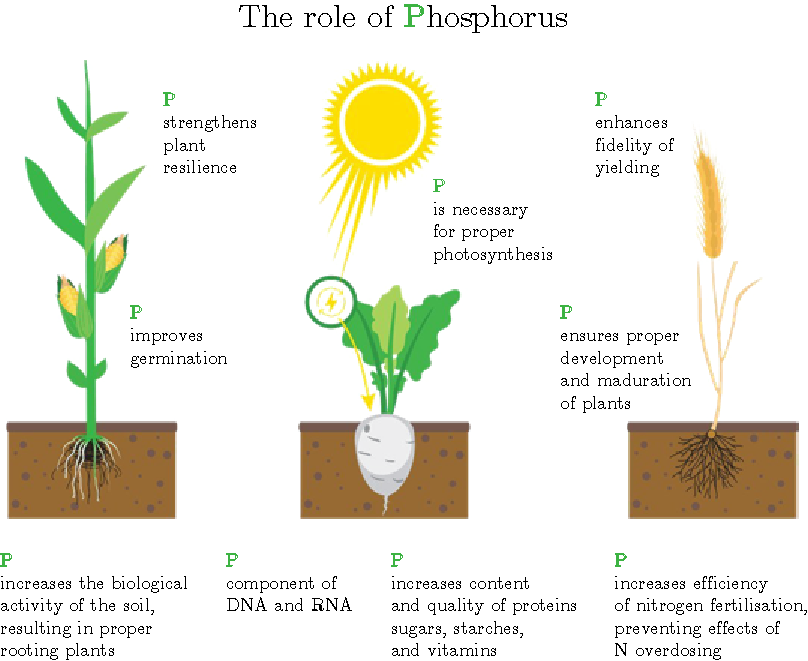
\includegraphics[width=0.7\textwidth]{Figures/PhosphorusPlantRoles.pdf}
     \caption{Phosphorus is an essential nutrient for proper growth of plants with  different functions shown in the figure. Reproduced from \cite{fertilizers}.}
     \label{fig:Phos}
 \end{figure}
 
%%%%%%%%%%%%%%%%%%%%%%%%%%%%%%%%%%%%%%%%%%%%%%%%%%%%%%%%%%%%%%%%%%
%%%%%%%%%%%%%%%%%%%%%%%%%%%%%%%%%
\subsection{Dynamics at the root}

Once the motivation to this project has been established, let us introduce the plant system we are going to be working with. First, we will briefly explain how plant roots interact with the soil around them in order to gather nutrients, and then we will consider the work in \cite{Ptashnyk-2011} to produce a mathematical model of this process.
 

%%%%%%%%%%%%%%%%%%%%%%%%%%%%%%%%%
%%%%%%%%%%%%%%%%%%%%%%%%%%%%%%%%%
%%%%%%%%%%%%%%%%%%%%%%%%%%%%%%%%%
\subsubsection{Root exudation and absorption}

When a plant germinates from a seed, it puts roots out into the soil around and below it. For many plants, the growth of the roots results in a large system of roots.
Some root systems are made up of many first order roots which contribute equally to nutrient gathering, while others are made up of a single first order root, which dominates the system, and other smaller second order roots, which contribute in smaller amounts, along with root hairs. 
The growth of roots and root hairs can be affected by the soil environment in which the plant is growing, see Figure \ref{fig:roots}.

Each root is made up of many layers of different kinds of tissue. What is important for our model is the existence of a cell wall and membrane that nutrients must pass through to be absorbed and used by the plant for various purposes \cite{PALLARDY2008255}. The root tip is covered by a single shell-like covering called the root cap. The root cap allows the root to push down into the soil without any important parts of its surface being damaged in the process. Because of its protective purpose, the root cap is tougher than the rest of the root \cite{haberlandt1914}. In what follows, we will consider the root cap to be inactive in the processes of exudation and nutrient uptake, and we will model only the interaction with the rest of the root.
Behind the root cap, there is a zone of exudation within which the plant may secrete certain chemicals out into the soil. These chemicals may break down nutrient compounds in the soil that cannot be absorbed directly, helping the plant to utilise them \cite{10.3389/fpls.2019.00157}.


\begin{figure}
\centering
\begin{minipage}{.45\textwidth}
    \centering
    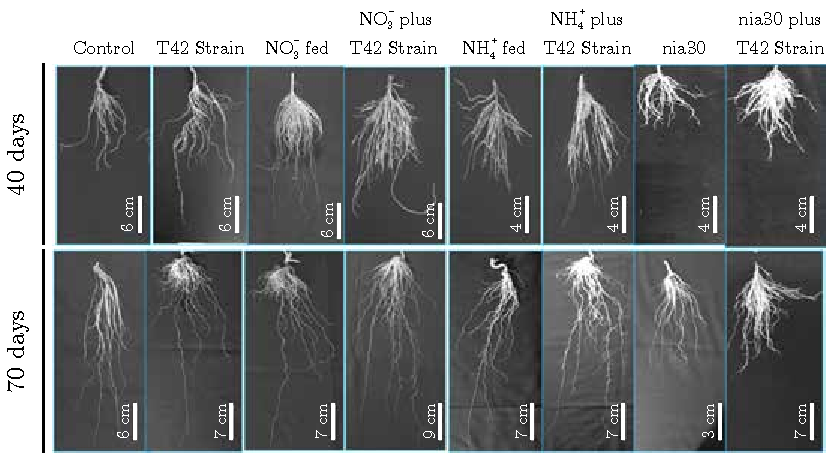
\includegraphics[width=\linewidth]{Figures/rootMorphology.pdf}
    \caption{ Different root responses to varying nutrient and moisture content in the soil, reproduced from \cite{PURNOBASUKI20182012}.}
    \label{fig:roots}
\end{minipage}%
\hfill
\begin{minipage}{.45\textwidth}
  \centering
    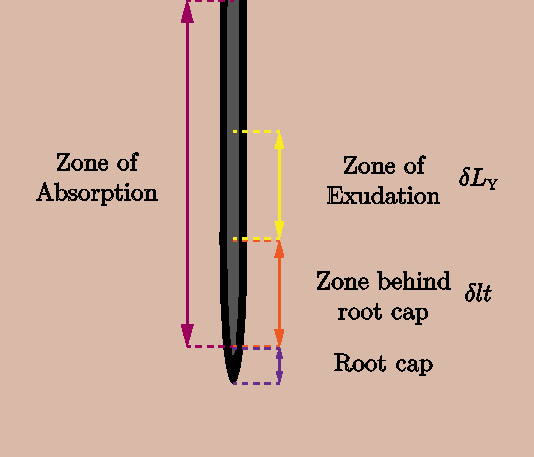
\includegraphics[width=.6\textwidth]{Figures/ZonesDiagram-plot.pdf}
    \caption{Diagram showing the zones of various activity on an example plant root.}
    \label{fig:zones}
\end{minipage}
\end{figure}

% There is then another zone, that of absorption. 
Another zone of the root important for our model is the absorption zone. In some plants, the whole root may absorb nutrients, while in others, absorption is limited to a smaller portion of the root surface. This is similar to the zone of exudation which in some plants may be very large and in others is limited to a very small region \SI{2}{cm} behind the root cap. This is portrayed in Figure \ref{fig:zones} along other key zones of a sample root.

Within the absorption zone, roots absorb many different elements from the soil. While the model in \cite{Ptashnyk-2011} focuses on zinc uptake, our primary interest is the uptake of phosphorus. Both of these nutrients can be highly deficient in many soil types and interact similarly with different exudates.



%%%%%%%%%%%%%%%%%%%%%%%%%%%
%%%%%%%%%%%%%%%%%%%%%%%%%%%
\subsubsection{Interaction of exudates with soil}

% Now that we have discussed the sections of the root and how they act we can consider the ways in which they interact with our soil solution. 
% Lets consider the mechanisms at work between the root and the soil solution with interaction between our exudates and the nutrients we are considering. 
In the case of \ce{Zn}  gathering, the plant exudes a phytosiderophore, deoxymugineic acid (\ce{DMA}), which acts to increase the uptake of \ce{Zn} from soils in the form of \ce{Zn^{2+}} and \ce{Zn-DMA} at the root surface, see Figure \ref{fig:Zinc} for a sketch of this process. In the case of phosphorus, the interaction is a little more complex. First, studies have shown that in soil with limited \ce{P} availability, exudation of citrate by plant roots has improved \ce{P} solubilisation in soils \textcolor{red}{explain why this works} allowing the inorganic \ce{P} to move from solid soil into soil solution. The presence of nutrients in soil solution is critical for plants as the nutrients get to the root surface by processes of diffusion and mass transport (transport of ions in the soil solution) \cite{Reichardt2020}.
% , where it moves by diffusion and convection which enables the root to absorb it.
Then we have the exudation of phytase enzymes which are responsible for the process of mineralising \ce{P}, i.e., converting organic \ce{P} into inorganic \ce{P} which can then be more easily processed by the plant. Most importantly, research has shown that working in tandem, citrate, and phytase have a much larger effect on \ce{P} absorption than we can currently explain, thus we have chosen to model the exudation of both rather than taking models of each single exudate by itself \cite{giles_george} \textcolor{red}{figure showing this effect?}.

\begin{figure}[h]
\centering
\begin{subfigure}[t]{0.35\textwidth}
    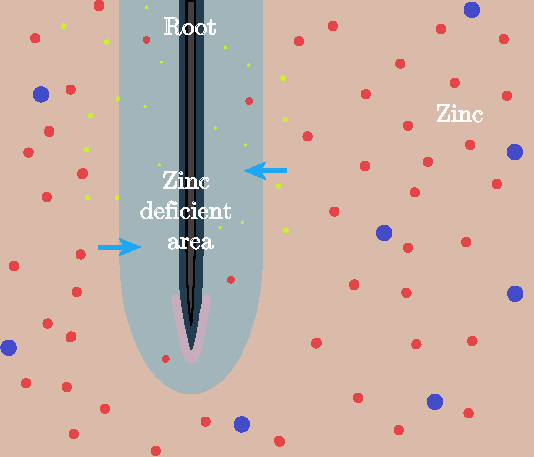
\includegraphics[width=\textwidth]{Figures/RootZincDiagram.pdf}
    \caption{}
    \label{fig:Zinc}
\end{subfigure}
\qquad
\begin{subfigure}[t]{0.35\textwidth}
    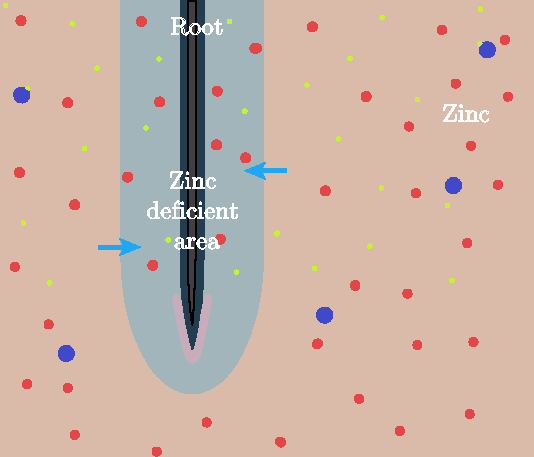
\includegraphics[width=\textwidth]{Figures/RootZincDiagram2.pdf}
    \caption{}
    \label{fig:my_label}
\end{subfigure}
\caption{Diagrams showing the dynamics of the exudate \ce{DMA} (green) with \ce{Zn} (red) in the soil; (a) \ce{DMA} improves \ce{Zn} solubility and causes it to move into the deficient area, presence of microbes (purple); (b) movement of \ce{Zn} in response to \ce{DMA} exudation and the consumption of \ce{DMA} by microbes.}
\end{figure}

\begin{figure}[!htb]
     \centering
     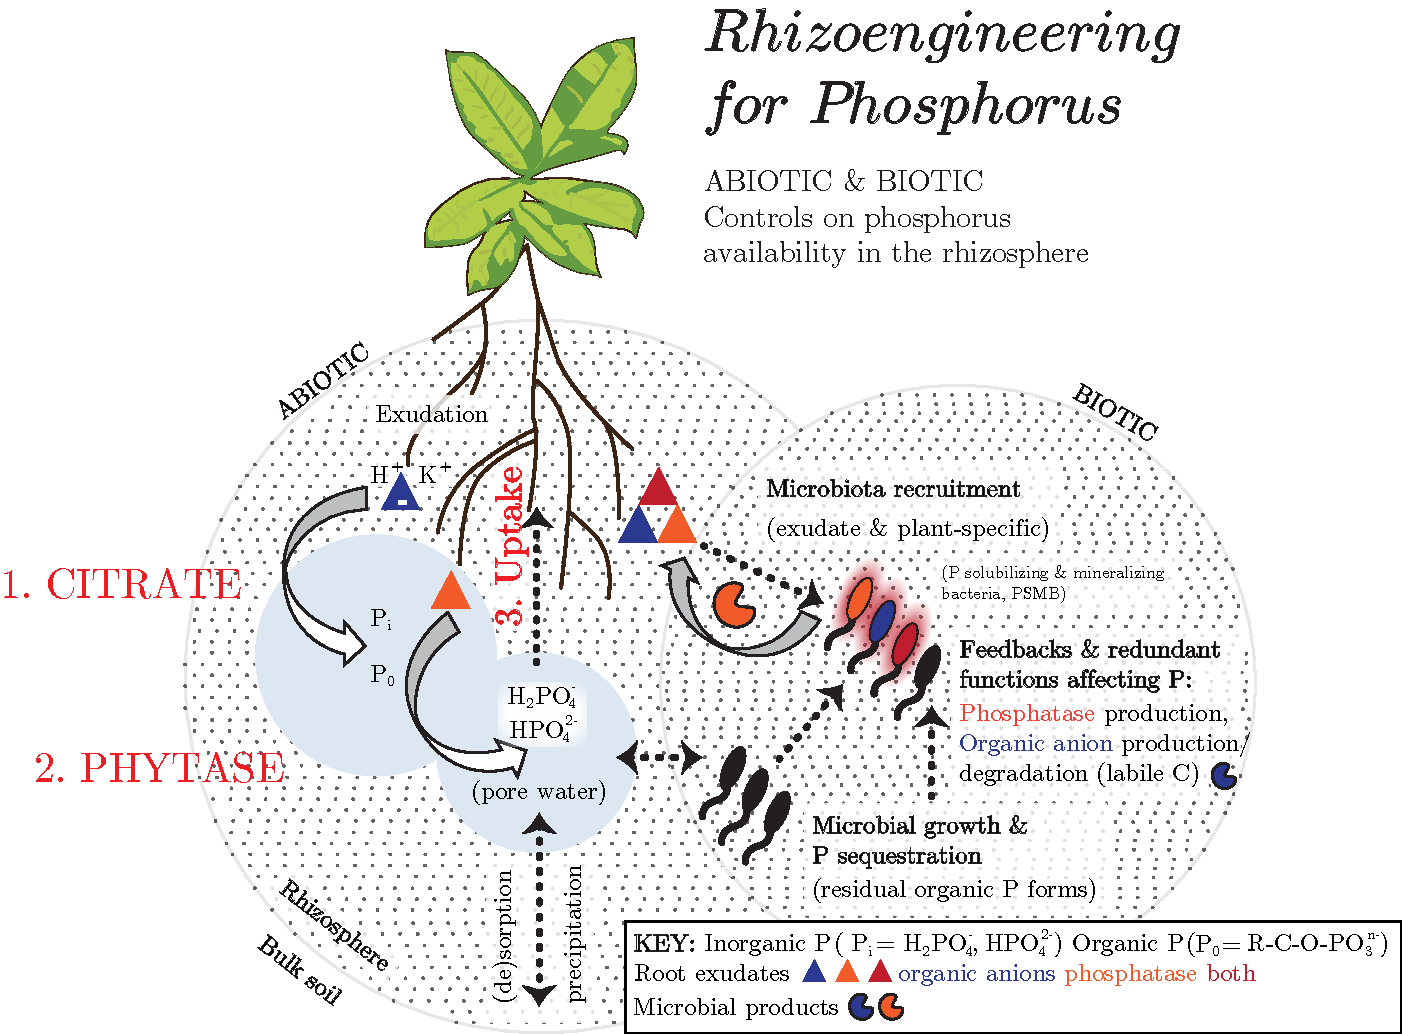
\includegraphics[width=0.7\textwidth]{Figures/Rhizoengineering.pdf}
     \caption{Role of citrate and phytase in the rhizosphere of a plant. Figure obtained by private communication with Tim George. }
     \label{fig:CitPhys}
 \end{figure}

%%%%%%%%%%%%%%%%%%%%%%%%%%%%%%%%%
%%%%%%%%%%%%%%%%%%%%%%%%%%%%%%%%%
\subsection{Base model formulation}
\label{sec:bio_basemodel}

We now present the model of \cite{Ptashnyk-2011} which considers the way rice plants access \ce{Zn} in \ce{Zn}-deficient soils. The paper models the mechanism of \ce{DMA} exudation which allows rice roots to access \ce{Zn} and form \ce{Zn-DMA} which is solubilised as explained in the previous sections. Let $X$ be the amount of the micronutrient metal \ce{Zn} and $Y$ the amount of exuded phytosiderophore \ce{DMA}. All parameters following in this section are described in Table \ref{t:First-model-params}. 
%The soil is modelled as a mixture of soil liquid and solid soil particles,
The equations model the movement of $X$ and $Y$ by diffusion and convection through the soil pore solution, allowing for adsorption and desorption to occur on soil surfaces and diffusion only within the soil solution. 
The concentrations of $X$ and $Y$ in the soil solution are marked by $X_L$ and $Y_L$, while their concentrations in the soil solid are $X_S$ and $Y_S$.
%We can split $X$ and $Y$ into the amount of each in he different states, let $X_L$, $Y_L$ be the concentrations of \ce{Zn} and \ce{DMA} in solution and $X_S$, $Y_S$ are the concentrations in soil solids. 
Thus the following conservation equations for $X$ and $Y$ are proposed:
\begin{equation}
\begin{aligned}
    \partial_t(\theta X_L+X_S)&=\nabla \cdot (D_X\nabla X_L-\nu X_L)-g_X,\\
    \partial_t(\theta Y_L+Y_S)&=\nabla \cdot (D_Y\nabla Y_L-\nu Y_L)-g_Y.
    \label{eq:1}
\end{aligned}
\end{equation}
%with parameters as summarised in Table \ref{t:First-model-params}. 
We can then derive equilibrium conditions between the soil particles and solution. %Simultaneously, we know that at this equilibrium there will be no change in the amount of \ce{DMA} or \ce{Zn} in solution, thus
At equilibrium describing fast absorption we have
\begin{equation}
    \begin{aligned}
        \partial_t X_s&=\beta_1X_L-\beta_2X_S-\beta_3X_SY_L=0,\\
        \partial_t Y_S&=\gamma_1Y_L-\gamma_2Y_S-\gamma_3Y_SX_L=0,
    \end{aligned}
    \label{eq:2}
\end{equation}
with $\beta_1,\beta_2,\beta_3,\gamma_1,\gamma_2,\gamma_3$ being the reaction rate coefficients.
By differentiating the resulting algebraic equations in \eqref{eq:2} and substituting the expressions for $X_S$ and $Y_S$ into the system \eqref{eq:1}, we obtain the reduced system of parabolic equations
\begin{subequations}
\label{eq:system-Zinc}
\begin{align}
    \left( \theta + \frac{b_X}{1 + \kappa_X b_X Y_L} \right) \partial_t X_L - \frac{\kappa_X b_X^2 X_L}{(1+\kappa_X b_X Y_L)^2} \partial_t Y_L &=
    \nabla \cdot ( D_X \nabla X_L - \nu X_L  ) - g_X,
    \label{eq:sys-Zn-X-Omega}
    \\
    \left( \theta + \frac{b_Y}{1 + \kappa_Y b_Y X_L} \right) \partial_t Y_L - \frac{\kappa_Y b_Y^2 Y_L}{(1+\kappa_Y b_Y X_L)^2} \partial_t X_L &=
    \nabla \cdot ( D_Y \nabla Y_L - \nu Y_L  ) - g_Y.
    \label{eq:sys-Zn-Y-Omega}
\end{align}
Having derived the dynamics of $X_L$ and $Y_L$ in soil, we will now insert a plant root into the system by determining boundary conditions of our domain.
The concentrations of $X_L$ and $Y_L$ depend upon the pair of spatial variables in $(r,z) \in \mathbb{R}^2$ which measure radial distance from the center of the root and length from the soil surface respectively as shown in figure \ref{fig:geom}, respectively. Furthermore, we specify the domain by restricting to $r \in [a,x]$ where $a$ is the diameter of the root and $x$ is radius of zone of root influence. Notice that we are modelling the region starting at the surface of the root and the root itself is not part of the domain. In the vertical direction, we will restrict to $z \in [-L_{t_{max}},0]$ as we assume the root growing into the downward direction, reaching length of the active zone of the root $L_{t_{max}}$ at the end of simulation at some time $t_{max}$. We note that we consider the active zone of the root to be the zone up to where the root cap begins, see Figure \ref{fig:zones}.
The presence of a single plant root on one vertical edge (on the left-hand side of the domain) results in 
\begin{align}
    D_X \partial_r X_L - \nu X_L &= \alpha X_L & \text{at } r &= a, \quad z \in [-L, -(L - \delta L_X)], \label{eq:sys-Zn-X-Gamma-a} 
    \\
    D_Y \partial_r Y_L - \nu Y_L &= -F_Y(t) &\text{at } r &= a, \quad z \in [-(L - \delta lt), -(L - \delta lt - \delta L_Y)].  \label{eq:sys-Zn-Y-Gamma-a} 
\end{align}
For the rest of the boundary, we have zero-flux conditions; i.e., in the case of the other edge \( r = x\), this is just
\begin{equation}
\label{eq:sys-Zn-X-Gamma-x}
     D_X \partial_r X_L - \nu X_L = 0
    \qquad\text{and}\qquad
    D_Y \partial_r Y_L - \nu Y_L = 0.
\end{equation}
\end{subequations}
Boundary condition \eqref{eq:sys-Zn-Y-Gamma-a}  represents the exudation of \ce{DMA} from a region on the root surface of length $\delta L_Y$ located at distance $\delta lt$ behind the end of root cap, while the absorption of \ce{Zn} from the soil surrounding the root is captured by \eqref{eq:sys-Zn-X-Gamma-a} at region of length $\delta L_X$ behind the start of root cap. In all the simulations in this report we will assume nutrient absorption along the whole root except the root cap, i.e. $\delta L_X = L$, but keep the interval for absorption in the general form as above. Although the exudation rate $F_Y(t)$ was initially modelled to be dependent of time, the conclusions of the original paper allow us to eventually keep it as a constant over 24 hours.



\begin{table}[!htb]
\begin{center}
\fontsize{9.5}{7}\selectfont
\setlength{\tabcolsep}{5.pt}
\def\arraystretch{1.5}
\begin{tabular}{cl}
\toprule
    \bf Symbol & \multicolumn{1}{c}{\bf Meaning}
    %
    \\ \midrule
    $\theta$ & Solution volume fraction \\
    $f$ & Diffusion impedance factor \\
    $D_{LX}$ & Diffusion coefficient of nutrient $X$  in free solution \\
    $D_{LY}$ & Diffusion coefficient of exudate $Y$  in free solution \\
    $D_X$ & Diffusion of the the nutrient $X$ in the soil, $D_X = D_{LX} \theta f$  \\  
	$D_{Y}$ &  Diffusion of the exudate $Y$ in the soil, $D_{Y} = D_{LY} \theta f$  \\ 
	$\nu$ & Water flux\\
	$g_X$ & Function for the immobilisation of nutrient $X$ \\
	$g_{Y}$ & Function for decomposition of the exudate $Y$ \\
	$b_X$ & Buffer power of $X$ \\
	$b_{Y}$ & Buffer power of $Y$ \\
	$\kappa_{X}$ & $X$ - $Y$ interaction coefficient \\
	$\kappa_{Y}$ & $Y$ - $X$ interaction coefficient\\
	$\alpha $ & $X$-absorbing power of root \\
	$F_{Y} $ & Rate of $Y$ exudation  \\
	$L$ & Length of root at certain time, increases at rate $G$ \\
	$\delta L_{X}$ & Length of $X$ uptake zone \\
	$\delta L_{Y}$ & Length of $Y$ exudation zone  \\	
	$\delta lt$ & Length of the zone between the end of exudation zone\\& and the beginning of root cap \\
	$a$ & Root radius \\
	$x$ & Radius of zone of root influence \\
\bottomrule
\end{tabular}
\caption{Table of parameters and their meanings for base model.
\label{t:First-model-params}}
\end{center}
\end{table}

\begin{figure}[!h]
    \centering
    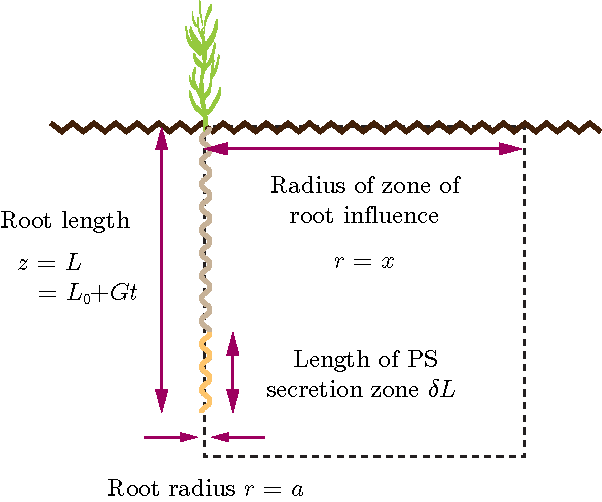
\includegraphics[scale=0.7]{Figures/First-plot.pdf}
    \caption{Sketch of the domain for system with one plant as modelled in \cite{Ptashnyk-2011} with $L_0$ being the length of root at the beginning of simulation and $G$ being the growth rate of the root. The root portrayed is curly for illustration purposes.}
    \label{fig:geom}
\end{figure}










\newpage
%%%%%%%%%%%%%%%%%%%%%%%%%%%%%%%%%%%%%%%%%%%%%%%%%%%%%%%%%%%%%%%%%%%%%%%%%%%%%%%%%%%%%%%%%%%%%%%%%%%%%%%%%%%%%%%%%%%%%%%%%%%%%%%%%%%%%%%%%%%%%%%%%%%%%%%%%%%%%%%%%%%%%%%%%%%%%%%%%%%%%%%%%%%%%%%%%%%%%%%%%%%%%%%%%%%%%%%%%%%%%%%%%%%%%%%%%%%%%%%%%%%%%%%%%%%%%%%

\section{Base model experimentation}
\label{sec:Base}


In this section, we will continue studying the original model from \cite{Ptashnyk-2011}. First, an extension for two roots to model a root secreting an exudate $Y$ in order to facilitate absorption of a nutrient $X$ from the soil. Second, a non-dimensionalisation procedure is presented. Third, a numerical approach is discussed to approximate solutions of the coupled partial differential equation systems. Finally, we finish with a set of numerical experiments for the original model \eqref{eq:system-Zinc} and the two roots model.

%For the purpose of the next sections, we now generalise the system introduced in section \ref{sec:bio_basemodel} to model a root secreting an exudate $Y$ in order to facilitate absorption of a nutrient $X$ from the soil. 

\begin{comment}
We will work with the system of PDEs
\begin{subequations}
\label{eq:system-Zinc}
\begin{align}
    \left( \theta + \frac{b_X}{1 + \kappa_X b_X Y_L} \right) \partial_t X_L - \frac{\kappa_X b_X^2 X_L}{(1+\kappa_X b_X Y_L)^2} \partial_t Y_L &=
    \nabla \cdot ( D_X \nabla X_L - \nu X_L  ) - g_X
    \label{eq:sys-Zn-X-Omega}
    \\
    \left( \theta + \frac{b_Y}{1 + \kappa_Y b_Y X_L} \right) \partial_t Y_L - \frac{\kappa_Y b_Y^2 Y_L}{(1+\kappa_Y b_Y X_L)^2} \partial_t X_L &=
    \nabla \cdot ( D_Y \nabla Y_L - \nu Y_L  ) - g_Y;
\end{align}
where $X_L(r,z)$ and $Y_L(r,z)$ are concentrations of the two nutrients in the soil solution subject to the boundary conditions
\begin{align}
    D_X \partial_r X_L - \nu X_L &= \alpha X_L & \text{at } r &= a, z \in [-L, -(L - \delta L_X)],
    \label{eq:sys-Zn-X-Gamma-a}
    \\
    D_Y \partial_r Y_L - \nu Y_L &= -F_Y(t) &\text{at } r &= a, z \in [-(L - \delta lt), -(L - \delta lt - \delta L_Y)],
\end{align}
where $L = L_0 + G t$. For the rest of the boundary, we have zero-flux conditions; i.e., in the case \( r = x\), this is just
\begin{align}
    D_X \partial_r X_L - \nu X_L = 0
    \label{eq:sys-Zn-X-Gamma-x}
    \qquad\text{and}\qquad
    D_Y \partial_r Y_L - \nu Y_L = 0.
\end{align}
Moreover, $r \in [a,x]$, 
%with $x = (\pi L_V)^{1/2}$, % commented out because we want to keep it general 
and $z \in [0, L_{t_{\mathrm{max}} }]$. The meaning of these parameters is presented in Table \ref{t:First-model-params}. 
\end{subequations}
\end{comment}

%Initially, we will consider there is no exudate $Y_L$ in the rhizosphere, i.e. $Y_L = Y_L^0 = 0$ at $t=0$, and the initial condition for the nutrient, $X_L = X_L^0$ at $t=0$, will be set according to the nutrient and specified in the sections for numerical experiments.


%%%%%%%%%%%%%%%%%%%%%%%%%%%%%%
%%%%%%%%%%%%%%%%%%%%%%%%%%%%%%
%%%%%%%%%%%%%%%%%%%%%%%%%%%%%%
\subsection{Extension to two roots}
\label{sec:basemodel_extension}


We can extend model \eqref{eq:system-Zinc} by applying symmetry in the boundary conditions to consider another root in the domain, see Figure \ref{fig:system-Zinc}. Since we are not making any changes to the system itself, we are still limited to modelling one exudate and nutrient being absorbed. Nonetheless, the generalisation of the boundary conditions allow us to adjust the characteristics of the second root, namely the uptake power, exudation rate, growth rate, and exudation and uptake zones at the root. The extended set of boundary conditions is
\begin{subequations}
\label{sys:extension-two-roots}
\begin{align}
    D_X \partial_r X_L - \nu X_L &= \alpha_1 X_L & \text{at } r &= a, & z &\in [-L_1, -(L_1 - \delta L_{X,1})], \\
    D_Y \partial_r Y_L - \nu Y_L &= -F_{Y,1}(t) &\text{at } r &= a, &z &\in [-({L}_1 - \delta {lt}_1), -({L}_1 - \delta {lt}_1 - \delta {L}_{Y,1})], \\
    D_X \partial_r X_L - \nu X_L &= -\alpha_2 X_L & \text{at } r &= w+a, &z &\in [-L_2, -(L_2 - \delta L_{X,2})], \\
    D_Y \partial_r Y_L - \nu Y_L &= F_{Y,2}(t) &\text{at } r &= w+a, &z &\in [-({L}_2 - \delta {lt}_2), -({L}_2 - \delta {lt}_2 - \delta {L}_{Y,2})],
\end{align}
\end{subequations}
where the parameters bear the same meanings as in Table \ref{t:First-model-params}, and they are indexed by the root they correspond to; i.e., 1 for the left-hand side of the domain and 2 for the right-hand side of the domain. We note that in this general setting the two plants can have different growth rates, i.e. $L_1 = L_{0,1} + G_1t$, $L_2 = L_{0,2} + G_2t$, where $L_{0,1}$, $L_{0,2}$ are root lengths at the beginning of the simulation. The second root is located at $r = w+a$ where $w$ is the width of the space between the two roots. This distance can be manipulated so that the zones of root influence intersect with each other; thus allowing to model intercropping and the effect of the proximity of two roots on each other. For the rest of the boundary we consider zero-flux boundary conditions.


\begin{figure}[h]
    \centering
    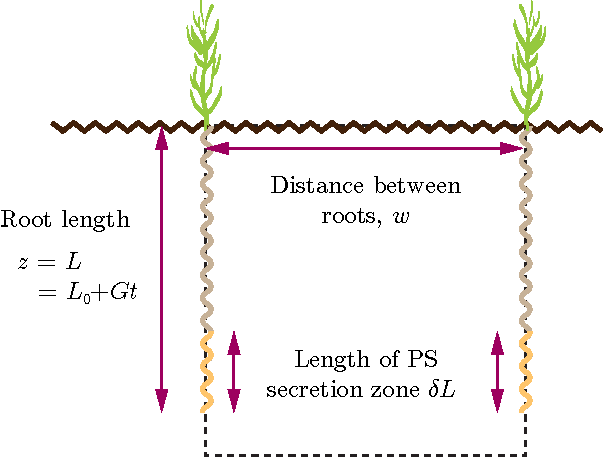
\includegraphics[scale=0.7]{Figures/Second-plot.pdf}
    \caption{Sketch of the domain for system with two plants and one exudate.}
    \label{fig:system-Zinc}
\end{figure}


%%%%%%%%%%%%%%%%%%%%%%%%%%%%%%%%%%%%%%%%%
%%%%%%%%%%%%%%%%%%%%%%%%%%%%%%%%%%%%%%%%%
\subsection{Non-dimensionalisation}
\label{2-Base-Scaling}

%A drawback of model \eqref{eq:system-Zinc} is that numerical schemes for solving it might perform poorly if the parameters associated to the model are too small. This is actually the case, in the setting of Zinc uptake. As a result, 
As a standard procedure,
we will appropriately scale the variables of model \eqref{eq:system-Zinc} and its two-root extension \eqref{sys:extension-two-roots}. For this end, we introduce the following relations
\[
    r = \varepsilon_r \hat{r} + a,
    \qquad
    z = \varepsilon_z \hat{z},
    \qquad
    t = \varepsilon_t \hat{t},
    \qquad
    X_L = \varepsilon_x \hat{x},
    \qquad
    Y_L = \varepsilon_y \hat{y};
\]
where \( \varepsilon_r, \varepsilon_z, \varepsilon_t, \varepsilon_x, \varepsilon_y\) are scaling constants to be determined, and \(\hat{r}, \hat z, \hat t, \hat x, \hat y\) are non-dimensional variables.
Clearly, we have the relation \(X_L(r,z) = \varepsilon_x \hat{x} (\varepsilon_r \hat r + a, \varepsilon_z \hat z) = \varepsilon_x \hat{x} \big( \varepsilon_r^{-1} (r-a) , \varepsilon_z^{-1} z\big) \) and similarly \(Y_L (r,z) = \varepsilon_y \hat{y} \big( \varepsilon_r^{-1} (r-a), \varepsilon_z^{-1} z \big)\). Using this, we see that the gradient operator is also scaled as
\[
    \nabla X_L =
    \begin{pmatrix}
        \nicefrac{1}{\varepsilon_r} & 0 \\
        0 & \nicefrac{1}{\varepsilon_z}
    \end{pmatrix}
    \hat{\nabla} \varepsilon_x \hat{x},
    \qquad \text{with} \qquad
    \hat{\nabla} = 
    \begin{pmatrix}
        \pd{ }{\hat r}
        &
        \pd{ }{\hat z}
    \end{pmatrix}^\top .
\]
%The scaled equations are easy to determine. For instance,  \eqref{eq:sys-Zn-X-Omega} is measured in \si{M.s^{-1}}, which are the units that \(\varepsilon_x\) and \(\varepsilon_t^{-1}\) correspond to. 
For the left-hand side of \eqref{eq:sys-Zn-X-Omega} we have that
\begin{align}
    \left( \theta + \frac{b_X}{1 + \kappa_X b_X Y_L} \right) \partial_t X_L &= \frac{\varepsilon_x}{\varepsilon_t} \left( \theta + \frac{b_X}{1 + \varepsilon_y \kappa_X b_X \hat{y}} \right)  \pd{\hat{x}}{\hat{t}}
    \\
    - \frac{\kappa_X b_X^2 X_L}{(1+\kappa_X b_X Y_L)^2} \partial_t Y_L &=
    -\frac{\varepsilon_x}{\varepsilon_t} \frac{\varepsilon_y \kappa_X b_X^2 \hat{x}}{(1+ \varepsilon_y\kappa_X b_X \hat{y})^2} \pd{\hat y}{\hat t}
\end{align}
The right-hand side requires some care. 
%As \(\nu\) is measured in \si{dm.s^{-1}}, w
We introduce the non-dimensional quantities \( \hat{\nu}_r\) and \( \hat{\nu}_z\) such that \( \nu = \nicefrac{\varepsilon_r}{\varepsilon_t} \hat{\nu}_r \) and \( \nu = \nicefrac{\varepsilon_z}{\varepsilon_t} \hat{\nu}_z \),
%. Likewise, \(D_X\) is measured in \si{dm^2.s^{-1}}, and we can proceed as before introducing 
and \(\hat{D}_{X,r}\) and \(\hat{D}_{X,z}\) 
%two non-dimensional constants 
such that \(D_{X} = \nicefrac{\varepsilon_r^2}{\varepsilon_t} \hat{D}_{X,r}\) and \(D_{X} = \nicefrac{\varepsilon_z^2}{\varepsilon_t} \hat{D}_{X,z}\). This way, we have that
\begin{align}
    \nabla \cdot ( D_X \nabla X_L - \nu X_L  )
    &=
    \begin{pmatrix}
        \nicefrac{1}{\varepsilon_r} & 0 \\
        0 & \nicefrac{1}{\varepsilon_z}
    \end{pmatrix}
    \hat{\nabla}
    \cdot
    \left( 
        D_X
        \varepsilon_x
        \begin{pmatrix}
        \nicefrac{1}{\varepsilon_r} & 0 \\
        0 & \nicefrac{1}{\varepsilon_z}
    \end{pmatrix}
    \hat{\nabla} \hat{x} - \nu \varepsilon_x \hat{x}
    \right)
    \notag
    \\
    &= \varepsilon_x
    \begin{pmatrix}
        \nicefrac{1}{\varepsilon_r} & 0 \\
        0 & \nicefrac{1}{\varepsilon_z}
    \end{pmatrix}
    \hat{\nabla}
    \cdot
    \left( 
        \begin{pmatrix}
         \nicefrac{\varepsilon_r}{\varepsilon_t} \hat{D}_{X,r} & 0 
         \\
        0 &  \nicefrac{\varepsilon_z}{\varepsilon_t} \hat{D}_{X,z}
    \end{pmatrix}
    \hat{\nabla} \hat{x} - \hat{x}
    \begin{pmatrix}
         \nicefrac{\varepsilon_r}{\varepsilon_t} \hat{\nu}_{r} 
         \\
        \nicefrac{\varepsilon_z}{\varepsilon_t} \hat{\nu}_{z}
    \end{pmatrix}
    \right)
    \notag
    \\
    &= \frac{\varepsilon_x}{\varepsilon_t}
    \hat{\nabla}
    \cdot
    \left( 
        \begin{pmatrix}
         \hat{D}_{X,r} & 0 
         \\
        0 &  \hat{D}_{X,z}
    \end{pmatrix}
    \hat{\nabla} \hat{x} - \hat{x}
    \begin{pmatrix}
         \hat{\nu}_{r} 
         \\
        \hat{\nu}_{z}
    \end{pmatrix}
    \right).
    \label{eq:divergence-non-dimen-x}
\end{align}
For \(g_X\) we 
%For \(g_X\) we can proceed as we did for \eqref{eq:divergence-non-dimen-x} by noticing that its measured in \si{M.s^{-1}} and 
introduce the non-dimensional quantity \( \frac{\varepsilon_x}{\varepsilon_t}\hat{g}_{x} = g_X\). Equation \eqref{eq:sys-Zn-Y-Omega} and the parameters involved follow a similar argument.





%%%%%%%%%%%%%%%%%%%%%%%%%%%%%%%%%
\subsubsection{Boundary and initial conditions}




Let us now discuss the non-dimensionalisation of the boundary conditions. For the one model root \eqref{eq:system-Zinc}, we have that \eqref{eq:sys-Zn-X-Gamma-a} is equivalent to
\[
    D_X \partial_r X_L - \nu X_L = 
    \frac{\varepsilon_r^2}{\varepsilon_t} \hat{D}_{X,r} \frac{\varepsilon_x}{\varepsilon_r} \pd{\hat{x}}{\hat{r}} - \frac{\varepsilon_r}{\varepsilon_t} \hat{\nu}_r \varepsilon_x \hat{x} = \frac{\varepsilon_r \varepsilon_x}{\varepsilon_t} \hat{\alpha} \hat{x}
    \qquad \text{at } r = a = a + \varepsilon_r \hat{r},\quad \varepsilon_z \hat{z} \in [-L, -(L - \delta L_X)],
\]
or equivalently
\begin{equation}
    \label{eq:sys-Zn-nond-a}
    \hat{D}_{X,r} \pd{\hat{x}}{\hat{r}} - \hat{\nu}_r \hat{x} = \hat{\alpha} \hat{x}
    \qquad \text{at } \hat{r} = 0, \quad \hat{z} \in [-\hat{L}, -(\hat{L} - \delta \hat{L}_x)];
\end{equation}
where we require \( \alpha = \nicefrac{\varepsilon_r}{\varepsilon_t} \hat{\alpha}\), \( \hat{L} = \varepsilon_z^{-1} L\), and \( \delta\hat{L}_x = \varepsilon_z^{-1} \delta L_X\). Likewise for \eqref{eq:sys-Zn-Y-Gamma-a}, we get %\(\hat{F}_y = \frac{\varepsilon_t}{\varepsilon_r \varepsilon_y} F_y \)
\begin{equation}
    \label{eq:sys-Zn-nond-b}
    \hat{D}_{Y,r} \pd{\hat{y}}{\hat{r}}  - \hat{\nu}_r \hat{y} = -\hat{F}_y(t)     \qquad\text{at } \hat{r} = 0, \quad \hat{z} \in [-(\hat{L} - \delta \widehat{lt}), -(\hat{L} - \delta \widehat{lt} - \delta \hat{L}_y)].
\end{equation}
Finally, condition \eqref{eq:sys-Zn-X-Gamma-x} is just
\begin{equation}
    \label{eq:sys-Zn-nond-x}
    \hat{D}_{X,r} \pd{\hat{x}}{\hat{r}} - \hat{\nu}_r \hat{x} = 0
    \qquad \text{at } \hat{r} = \frac{x-a}{\varepsilon_r}.
\end{equation}

Conditions \eqref{eq:sys-Zn-nond-a} and \eqref{eq:sys-Zn-nond-x} give us a hint of how we need to select \(\varepsilon_r\) and \(\varepsilon_z\). If we select \( \varepsilon_r = x-a\), then \( \hat{r} \) will be in the range \( [0,1]\). Similarly, if we pick \( \varepsilon_z = L_{t_{\max}}\), again \(\hat z \) will be in the range \([0,-1]\). This last selection implies that the maximum absolute value of \( \hat{L}\) should be \(1\) where we have
\[
    \hat{L} = \hat{L}(\hat t) = \frac{1}{\varepsilon_z} ( L_0 + G \varepsilon_t \hat t )
    = \hat{L}_0 + \hat{G} \hat t,
    \qquad 
    \hat{L}_0 = \varepsilon^{-1}_z L_0,
    \qquad
    \hat{G} = \varepsilon_t \varepsilon_z^{-1} G;
\]
and we can further select \( \varepsilon_t = t_{\max}\) to finally have \( \hat t\) in the range \( [0,1]\). 


The treatment is similar for the two roots model \eqref{sys:extension-two-roots}. Using similar transformations as for \eqref{eq:sys-Zn-nond-a} and \eqref{eq:sys-Zn-nond-b}, where we get
\begin{align}
    \hat{D}_{X,r} \pd{\hat{x}}{\hat{r}} - \hat{\nu}_r \hat{x} &= \hat{\alpha}_1 \hat{x}
    &\text{at } \hat{r} &= 0, \quad \hat{z} \in [-\hat{L}_1,-(\hat{L}_1 - \delta \hat{L}_{x,1})],
    \\
    \hat{D}_{Y,r} \pd{\hat{y}}{\hat{r}}  - \hat{\nu}_r \hat{y} &= -\hat{F}_{y,1}(t)     &\text{at } \hat{r} &= 0, \quad \hat{z} \in [-(\hat{L}_1 - \delta \widehat{lt}_1), -(\hat{L}_1 - \delta \widehat{lt}_1 - \delta \hat{L}_{y,1})],
    \\
    \hat{D}_{X,r} \pd{\hat{x}}{\hat{r}} - \hat{\nu}_r \hat{x} &= \hat{\alpha}_2 \hat{x}
    &\text{at } \hat{r} &= 1, \quad \hat{z} \in [-\hat{L}_2, -(\hat{L}_2 - \delta \hat{L}_{x,2})],
    \\
    \hat{D}_{Y,r} \pd{\hat{y}}{\hat{r}}  - \hat{\nu}_r \hat{y} &= -\hat{F}_{y,2}(t)     &\text{at } \hat{r} &= 1, \quad \hat{z} \in [-(\hat{L}_2 - \delta \widehat{lt}_2), -(\hat{L}_2 - \delta \widehat{lt}_2 - \delta \hat{L}_{y,2})].
\end{align}



Notice that in both models, we have selected scaling parameters such that the systems of partial differential equations are defined in \([0,1]\times [0,-1] \times [0,1]\). We will denote the scaled spatial domain as \(\Omega := [0,1]\times [0,-1]\) and its boundary \(\Gamma := \partial \Omega\).
Lastly, the initial conditions are scaled as \( (\hat{x}_0,\hat{y}_0) = (\varepsilon_x^{-1} X^0_L, \varepsilon_y^{-1} Y^0_L) \). 




%%%%%%%%%%%%%%%%%%%%%%%%%%%%%%
%%%%%%%%%%%%%%%%%%%%%%%%%%%%%%
%%%%%%%%%%%%%%%%%%%%%%%%%%%%%%
\subsection{Numerical Approximation}
\label{sec:Numerics-base}

In order to get numerical solutions of the coupled system of partial differential equations \eqref{eq:sys-Zn-X-Omega}--\eqref{eq:sys-Zn-Y-Omega} with boundary conditions \eqref{eq:sys-Zn-X-Gamma-a}--\eqref{eq:sys-Zn-Y-Gamma-a} or \eqref{sys:extension-two-roots}, we will use a splitting scheme.
%
Operator splitting is an attractive technique for solving coupled systems of differential equations, since complex equation systems may be split into smaller parts that are easier to solve.
As a result, this is a standard technique in the literature, for instance see \cite{Farrell-2019}, \cite{Sundnes-2006}, and the references therein. 
%The ideas of splitting coupled systems are not new in the literature.
%Previously, \cite{Farrell-2019} and \cite{Sundnes-2006} discussed a Leap-Frog-kind splitting method. Formally, the Strang splitting method aims to solve systems of the form
Defining \(u:= (\hat{x},\hat{y})\), we aim to solve a system of the form
\begin{equation}
    \label{ec:splitting}
	\pd{u}{t} = A_1(u) + A_2(u) 	\qquad \text{with} \qquad u(0) = u_0.
\end{equation}
As pointed out in \cite{Farrell-2019}, this is not trivial for software as FEniCS \cite{AlnaesBlechta2015a}. 
An approach, as shown in  \cite{Sundnes-2006}, is to select the operators \(A_1\) and \(A_2\) in \eqref{ec:splitting} such that we solve a linear system of PDEs for \(\hat{y}\) and then a subsequent linear system of PDEs for \(\hat{x}\). Here we must highlight that the representation of \(A_1\) and \(A_2\) in \eqref{ec:splitting} as a sum is merely for notational purposes.

The general approach is as follows. We start discretising the time domain with steps of length \(\Delta \hat{t}\). At step \(m = 0\), we solve the reduced problem 
\(
	\pd{\hat{y}}{t} = \tilde{A}_1(\hat{x}^m,\hat{y}; \hat{y}^m) 
\) with 
\( \hat{y}(m\Delta \hat{t}) = \hat{y}^m\),
and \( t\in [m\Delta \hat{t},(m+1)\Delta \hat{t}]\).
Here \(\tilde{A}_1(\hat{x}^m,\hat{y}; \hat{y}^m)\) indicates that nonlinearities in \(A_1\) are evaluated at \(\hat{x}^m\) and \(\hat{y}^m\) such that the resulting differential operator is linear in \(\hat{y}\).
The solution, labelled \(\hat{y}^{m+1}\), is then used to solve 
\(
	\pd{\hat{x}}{t} = \tilde{A}_2(\hat{x},\hat{y}^{m+1}; \hat{x}^m) 
\) with 
\( \hat{x}(m\Delta \hat{t}) = \hat{x}^m, \)
and \( t\in [m\Delta \hat{t},(m+1)\Delta \hat{t}]\). Then we repeat the process for the next steps. This is a Godunov-like splitting, which is a first order approximation \cite{Sundnes-2006}. 

\begin{comment}
Here, we discretise the time domain with steps of length \(\Delta t\) and start solving the reduced problem
\(
	\pd{v}{t} = A_1(v) 	\text{ with }  v(0) = u_0
\)
for \( t\in [0,\nicefrac{\Delta t}{2}]\). Then we solve
\(
	\pd{w}{t} = A_2(w) 	\text{ with }  v(0) = v(\nicefrac{\Delta t}{2})
\)
for \( t\in [0,\Delta t]\). Finally, we solve
\(
	\pd{v}{t} = A_1(w) 	 \text{ with } v(\nicefrac{\Delta t}{2}) = w(\Delta t)
\)
for \( t\in [\nicefrac{\Delta t}{2},\Delta t]\). It turns out that this approach delivers a solution second-order accuracy scheme, which can be proved with a Taylor expansion. 
\end{comment}

Additionally, we will approximate the time derivatives using simple backward differences. The explicit form of the resulting numerical scheme will be presented using a variational expression defined over the spatial domain \(\Omega\). 




%%%%%%%%%%%%%%%%%%%%%%%%%%
%%%%%%%%%%%%%%%%%%%%%%%%%%
\subsubsection{Non-dimensionalised variational expressions}


The existence of a solution to the model \eqref{eq:system-Zinc} and its extension with boundary conditions \eqref{sys:extension-two-roots} is presented in Section \ref{sec:Existence}. 
%
For now, let us suppose that there is a sufficiently smooth solution pair $(\hat x, \hat y)$ for each time \(\hat{t}\in [0,1]\). Now, let us fix \(\hat{t} \in (0,1)\). Now, introduce the nonlinear terms
\begin{align}
    A(\hat{y}) &= \theta + \frac{b_X}{1 + \hat{\kappa}_X b_X \hat{y}},
    &
    B(\hat{x},\hat{y}) &= \frac{\hat{\kappa}_X b_X^2 \hat{x}}{(1+\hat{\kappa}_X b_X \hat{y})^2},
    \\
    C(\hat{x}) &= \theta + \frac{b_Y}{1 + \hat{\kappa}_Y b_Y \hat{x}},
    &
    E(\hat{x},\hat{y}) &= \frac{\hat{\kappa}_Y b_Y^2 \hat{y}}{(1+\hat{\kappa}_Y b_Y \hat{x})^2};
\end{align}
where we have used the scaled constants \(\hat{\kappa}_X = \varepsilon_y \kappa_X\), \(\hat{\kappa}_Y = \varepsilon_x \kappa_Y\). 

Multiply the scaled equations of the parabolic system by a $v \in \mathcal{C}^1 (\bar\Omega)$ function and integrate this with respect to the pair \((r,z)\) using the Lebesgue measure \(\mu\). Using the Divergence Theorem \cite{Evans-2010}, we have
\begin{equation}
\label{eq:var-time-base}
\begin{aligned}
    \int\limits_\Omega
    A(\hat y) \pd{\hat{x}}{\hat{t}} v 
    -
    B(\hat x, \hat y) \pd{\hat y}{\hat t} v
    \dif\mu
    &=
    -\int\limits_\Omega 
    \big( \hat{D}_x \hat{\nabla} \hat{x} - \hat{x}\hat{\nu}\big) \cdot \hat{\nabla} v \dif\mu
    -\int\limits_\Omega \hat{g}_x v \dif\mu
    +\int\limits_{\Gamma}    \big( \hat{D}_x \hat{\nabla} \hat{x} - \hat{x}\hat{\nu}\big) \cdot \vec{n}  v    \dif \sigma,
    \\
    \int\limits_\Omega
    C(\hat{x})  \pd{\hat{y}}{\hat{t}} v 
    -
    E(\hat{x},\hat{y})  \pd{\hat x}{\hat t} v
    \dif\mu
    &=
    -\int\limits_\Omega 
    \big(\hat{D}_y \hat{\nabla} \hat{y} - \hat{y}\hat{\nu} \big) \cdot \hat{\nabla} v \dif\mu
    -\int\limits_\Omega \hat{g}_y v \dif\mu
    +\int\limits_{\Gamma}  \big(\hat{D}_y \hat{\nabla} \hat{y} - \hat{y}\hat{\nu} \big) \cdot \vec{n} v    \dif \sigma;
\end{aligned}
\end{equation}
where $\Gamma$ is the boundary of $\Omega$, $\vec{n}$ its normal vector, and $\sigma$ the surface measure on $\Gamma$. Moreover, we have used the scaled quantities \(\hat{g}_x = \frac{\varepsilon_t}{\varepsilon_x} g_X \) and \( \hat{g}_y = \frac{\varepsilon_t}{\varepsilon_y} {g}_Y \), the constant scaled vector 
\(
    \hat{\nu} = (
    \begin{smallmatrix}
        \hat{\nu}_r
        &
        \hat{\nu}_z
    \end{smallmatrix})^\top
    =
    \nu \varepsilon_t (
    \begin{smallmatrix}
        {\varepsilon_r}^{-1}
        &
        {\varepsilon_z}^{-1}
    \end{smallmatrix})^\top,
\) 
and the constant matrices
\[
    \hat{D}_x = 
    \begin{pmatrix}
         \hat{D}_{X,r} & 0 
         \\
        0 &  \hat{D}_{X,z}
    \end{pmatrix}
    =
    D_X \varepsilon_t
    \begin{pmatrix}
         \varepsilon_r^{-2} & 0 
         \\
        0 &  \varepsilon_z^{-2}
    \end{pmatrix}
    ,\qquad
    \hat{D}_y = 
    \begin{pmatrix}
         \hat{D}_{Y,r} & 0 
         \\
        0 &  \hat{D}_{Y,z}
    \end{pmatrix}
    =
    D_Y \varepsilon_t
    \begin{pmatrix}
         \varepsilon_r^{-2} & 0 
         \\
        0 &  \varepsilon_z^{-2}
    \end{pmatrix}.
\]

The resulting equations for the model of \cite{Ptashnyk-2011} are
\begin{equation}
\label{eq:var-time-model-1}
\begin{aligned}
    \int\limits_\Omega
    A(\hat y) \pd{\hat{x}}{\hat{t}} v 
    -
    B(\hat x, \hat y) \pd{\hat y}{\hat t} v
    \dif\mu
    &=
    -\int\limits_\Omega 
    \big( \hat{D}_x \hat{\nabla} \hat{x} - \hat{x}\hat{\nu}\big) \cdot \hat{\nabla} v \dif\mu
    -\int\limits_\Omega \hat{g}_x v \dif\mu
    -\int\limits_{\Gamma_{x}}    \hat{\alpha} \hat{x} v    \dif \sigma,
    \\
    \int\limits_\Omega
    C(\hat{x})  \pd{\hat{y}}{\hat{t}} v 
    -
    E(\hat{x},\hat{y})  \pd{\hat x}{\hat t} v
    \dif\mu
    &=
    -\int\limits_\Omega 
    \big(\hat{D}_y \hat{\nabla} \hat{y} - \hat{y}\hat{\nu} \big) \cdot \hat{\nabla} v \dif\mu
    -\int\limits_\Omega \hat{g}_y v \dif\mu
    +\int\limits_{\Gamma_{y}}    \hat{F}_y v    \dif \sigma.
\end{aligned}
\end{equation}
Here we have identified the two segments \(\Gamma_{x} = \{0\}\times [-\hat{L}, -(\hat{L}-\delta \hat{L}_x)]$ and $\Gamma_{y} = \{0\}\times [-(\hat{L} - \delta \widehat{lt}), -(\hat{L} - \delta \widehat{lt} - \delta \hat{L}_y)]\). Observe that they depend on the current time \(\hat t\).

In contrast, the additional boundary terms in \eqref{sys:extension-two-roots} yield the following equations for the two-root extension:
\begin{equation}
\label{eq:var-time-model-2}
\begin{aligned}
    \int\limits_\Omega
    A(\hat y) \pd{\hat{x}}{\hat{t}} v 
    -
    B(\hat x, \hat y) \pd{\hat y}{\hat t} v
    \dif\mu
    &=
    \int\limits_\Omega 
    \big( \hat{x}\hat{\nu} - \hat{D}_x \hat{\nabla} \hat{x}\big) \cdot \hat{\nabla} v \dif\mu
    -\int\limits_\Omega \hat{g}_x v \dif\mu
    -\int\limits_{\Gamma_{1,x}}    \hat{\alpha}_1 \hat{x} v    \dif \sigma
    -\int\limits_{\Gamma_{2,x}}    \hat{\alpha}_2 \hat{x} v    \dif \sigma,
    %
    \\
    \int\limits_\Omega
    C(\hat{x})  \pd{\hat{y}}{\hat{t}} v 
    -
    E(\hat{x},\hat{y})  \pd{\hat x}{\hat t} v
    \dif\mu
    &=
    \int\limits_\Omega 
    \big(\hat{y}\hat{\nu} - \hat{D}_y \hat{\nabla} \hat{y} \big) \cdot \hat{\nabla} v \dif\mu
    -\int\limits_\Omega \hat{g}_y v \dif\mu
    +\int\limits_{\Gamma_{1,y}}    \hat{F}_{y,1} v    \dif \sigma
    +\int\limits_{\Gamma_{2,y}}    \hat{F}_{y,2} v    \dif \sigma.
\end{aligned}
\end{equation}
Here we have two segments for each root at time \(\hat t\). For the first, there are \(\Gamma_{1,x} = \{0\}\times [-\hat{L}_1,-(\hat{L}_1 - \delta \hat{L}_{x,1})]\) and \(\Gamma_{1,y} = \{0\}\times [-(\hat{L}_1 - \delta \widehat{lt}_1), -(\hat{L}_1 - \delta \widehat{lt}_1 - \delta \hat{L}_{y,1})] \). While for the second, we have \( \Gamma_{2,x} = \{1\}\times [-\hat{L}_2, -(\hat{L}_2 - \delta \hat{L}_{x,2})]\) and \(\Gamma_{2,y} = \{1\} \times [-(\hat{L}_2 - \delta \widehat{lt}_2), -(\hat{L}_2 - \delta \widehat{lt}_2 - \delta \hat{L}_{y,2})]\). 


Observe that \eqref{eq:var-time-model-1} and \eqref{eq:var-time-model-2} hold, by density, for any \(v \in H^1(\Omega)\). This assumes that \(\hat x\) and \(\hat y\), and their corresponding time derivatives, are defined pointwise in time. However, they no longer require to be defined pointwise for every \( (r,z) \in \Omega\).



%%%%%%%%%%%%%%%%%
%%%%%%%%%%%%%%%%%
\subsubsection{Time discretisation and decoupling}

As we mentioned before, we use a simple backward difference to approximate the time derivative.
To do this, we discretise the time domain by \(N+1\) uniform steps of length \(\Delta \hat{t}\). Here, let the superscript $n$ denote a quantity at time $\hat t_n$, where $n$ is an integer counting time levels, e.g. $\hat{x}^n$ is $\hat{x}$ evaluated at time level $n$. This yields
\begin{equation}
    \left(\pd{ \hat x}{\hat t}\right)^{n+1} \approx \frac{ \hat{x}^{n+1} - \hat{x}^n}{\Delta \hat t}
\end{equation}
for all \( n \in \{0,\ldots, N \}\).


Inserting this in the variational system, and applying the splitting technique discussed for \eqref{ec:splitting}, we get that the base model of \cite{Ptashnyk-2011} is approximated by the following scheme. Initialising \(\hat{x}^{0} = \hat{x}^{-1} = \hat{x}_0\) and \(\hat{y}^{0}=\hat{y}_0\), then for every \(n \in \{0,\ldots,N\}\): (A) Solve the variational problem of finding \( y^{n+1}\) such that
\begin{subequations}
\label{eq:var-time-model-1-alg}
\begin{equation}
\begin{aligned}
    \int\limits_\Omega
    C(\hat{x}^{n})  (\hat{y}^{n+1} - \hat{y}^{n}) v 
    &-
    E(\hat{x}^{n},\hat{y}^n)  (\hat{x}^{n} - \hat{x}^{n-1}) v
    \dif\mu
    \\
    &\qquad=
    \Delta \hat{t}
    \int\limits_\Omega 
    \big(\hat{y}^{n+1} \hat{\nu} - \hat{D}_y \hat{\nabla} \hat{y}^{n+1} \big) \cdot \hat{\nabla} v \dif\mu
    -\Delta \hat{t}\int\limits_\Omega \hat{g}_y^{n} v \dif\mu
    +\Delta \hat{t}\int\limits_{\Gamma_{y}^{n+1}}    \hat{F}_y v    \dif \sigma
\end{aligned}
\end{equation}
for every \(v\in H^1(\Omega)\). (B) Proceed on finding \( x^{n+1}\) such that it satisfies
\begin{equation}
\begin{aligned}
    %
    \int\limits_\Omega
    A(\hat y^{n}) (x^{n+1} - x^n) v 
    &-
    B(\hat x^{n}, \hat y^{n}) (y^{n+1} - y^{n}) v
    \dif\mu
    \\ &\qquad=
    \Delta \hat{t}\int\limits_\Omega 
    \big(\hat{x}^{n+1}\hat{\nu} - \hat{D}_x \hat{\nabla} \hat{x}^{n+1} \big) \cdot \hat{\nabla} v \dif\mu
    -\Delta \hat{t}\int\limits_\Omega \hat{g}_x^{n} v \dif\mu
    -\Delta \hat{t}\int\limits_{\Gamma_{x}^{n+1}}    \hat{\alpha} \hat{x}^{n+1} v    \dif \sigma
\end{aligned}
\end{equation}
\end{subequations}
for every \(v\in H^1(\Omega)\). (C) Until the iterations have finished, go back to step (A).


Correspondingly, the extension for two roots with boundary conditions \eqref{sys:extension-two-roots} is approximated by the following scheme. Initialising \(\hat{x}^{0} = \hat{x}^{-1} = \hat{x}_0\) and \(\hat{y}^{0}=\hat{y}_0\), then for every \(n \in \{0,\ldots,N\}\): (A) Solve the variational problem of finding \( y^{n+1}\) such that
\begin{subequations}
\label{eq:var-time-model-2-alg}
\begin{equation}
\begin{aligned}
    \int\limits_\Omega
    C(\hat{x}^{n})  &(\hat{y}^{n+1} - \hat{y}^{n}) v 
    -
    E(\hat{x}^{n},\hat{y}^n)  (\hat{x}^{n} - \hat{x}^{n-1}) v
    \dif\mu
    \\
    &=
    \Delta \hat{t} \Big(
    \int\limits_\Omega 
    \big(\hat{y}^{n+1} \hat{\nu} - \hat{D}_y \hat{\nabla} \hat{y}^{n+1} \big) \cdot \hat{\nabla} v \dif\mu
    -\int\limits_\Omega \hat{g}_y^{n} v \dif\mu
    +\int\limits_{\Gamma_{1,y}^{n+1}}    \hat{F}_{y,1} v    \dif \sigma
    +\int\limits_{\Gamma_{2,y}^{n+1}}    \hat{F}_{y,2} v    \dif \sigma \Big)
\end{aligned}
\end{equation}
for every \(v\in H^1(\Omega)\). (B) Proceed on finding \( x^{n+1}\) such that it satisfies
\begin{equation}
\begin{aligned}
    %
    \int\limits_\Omega
    A(\hat y^{n}) &(x^{n+1} - x^n) v 
    -
    B(\hat x^{n}, \hat y^{n}) (y^{n+1} - y^{n}) v
    \dif\mu
    \\ &=
    \Delta \hat{t} \Big( \int\limits_\Omega 
    \big(\hat{x}^{n+1}\hat{\nu} - \hat{D}_x \hat{\nabla} \hat{x}^{n+1} \big) \cdot \hat{\nabla} v \dif\mu
    -\int\limits_\Omega \hat{g}_x^{n} v \dif\mu
    -\int\limits_{\Gamma_{1,x}^{n+1}}    \hat{\alpha}_1 \hat{x}^{n+1} v    \dif \sigma
    -\int\limits_{\Gamma_{2,x}^{n+1}}    \hat{\alpha}_2 \hat{x}^{n+1} v    \dif \sigma \Big)
\end{aligned}
\end{equation}
\end{subequations}
for every \(v\in H^1(\Omega)\). (C) Until the iterations have finished, go back to step (A).

\vspace{1\baselineskip}
In both approximation schemes, each contributing subset of \(\Gamma\) is updated for the current time step. For instance, segment \(\Gamma_{1,y}^{n+1}\) is the segment \(\Gamma_{1,y}\) at time \( \hat{t}_{n+1} = (n+1)\Delta \hat t\).






%%%%%%%%%%%%%%%%%%%%%%%%%%%%%%%%%%%%%%%%%
\subsubsection{Implementation comments}



The varational problems in \eqref{eq:var-time-model-1-alg} and \eqref{eq:var-time-model-2-alg} will be solved with FEniCS \cite{AlnaesBlechta2015a} with its Python interface. The code and related files are available in the repository of this project as mentioned in Appendix \ref{app:one}.

%To numerically solve the system in FEniCS, we use the variational formulation discretised in time defined in the previous subsections. Since the problem is nonlinear, we can linearise it by using the solution computed in the previous time step. First, we solve the equation for $Y$, (insert eq), followed by the equation for $X$ \textcolor{red}{FINISH the computational formulation}.

In FEniCS, we define the boundaries as the edges of the rectangular domain. However, neither of our boundary conditions is valid on the whole edge but only on a part of it (along the whole root or a segment).
Let us consider the original model from \cite{Ptashnyk-2011} in its scaled version. Here the segments \(\Gamma_x\) and \(\Gamma_y\) are defined by indicator functions. 
The first indicator function should attain one along the whole root except the root cap (i.e. where the uptake of a nutrient happens). Thus, the indicator function should act on the interval 
\[
    0 \geq \hat{z} \geq -(\hat{L}_0 + \hat{G} \hat{t} ),
\]
as the root is growing downwards. We would prefer for the indicator function to not be a step function as its discontinuity is likely to cause numerical issues. Therefore, we opt for an $\arctan$ regularisation of the form
\begin{equation}
    I_1 (\hat z) = \frac{1}{\pi} \arctan\Big(c \big(\hat z + (\hat L_0 + \hat G \hat t) \big) \Big) + \frac{1}{2},
\end{equation}
where $c$ defines the steepness of the regularisation. The multiplication by $\frac{1}{\pi}$ and addition of $\frac{1}{2}$ sets the range of the function from $0$ to $1$ in the sense of $\lim_{\hat z \to \infty} I_1(\hat z) = 1$ and $\lim_{\hat z \to -\infty} I_1(\hat z) = 0$.

The second indicator function is for the exudation boundary condition at 
\[
    -(\hat L_0 + \hat G \hat t - \delta \widehat{lt} - \delta \hat L_y) \geq z \geq -(\hat L_0 + \hat G \hat t - \delta \widehat{lt}).
\]
Again we use a similar regularisation:
\begin{equation}
    I_2 (\hat z) = \frac{1}{\pi} \bigg[ \arctan\Big(c \big(\hat z + (\hat L_0 + \hat G\hat t -\delta \widehat{lt}) \big) \Big) - \arctan\big(c \big( \hat z+(\hat L_0 + \hat G \hat t - \delta \widehat{lt} - \delta \hat L_Y ) \big) \Big) \bigg].
\end{equation}
% (in the experiments we used both $d = 2$ cm and $\delta L_Y = 2$ cm, i.e. the plants is exuding at a 2 cm long region located 2 cm behind the root tip).

The regularised indicators $I_1(\hat z)$, $I_2(\hat z)$ can be mirrored easily to act on the second root in the system as their values do not depend on the $\hat r$ coordinate, with their parameters possibly adjusted to change the characteristics of the root as described in Section \ref{sec:basemodel_extension}.

\subsection{Numerical experiments}
Using parameters from table 1 in \cite{Ptashnyk-2011} we can consider what this two-root model tells us about rice plants grown in close proximity to each other.


\subsubsection{Original parameters}
 \begin{figure}[h]
     \centering
     \begin{subfigure}[t]{0.35\textwidth}\centering
     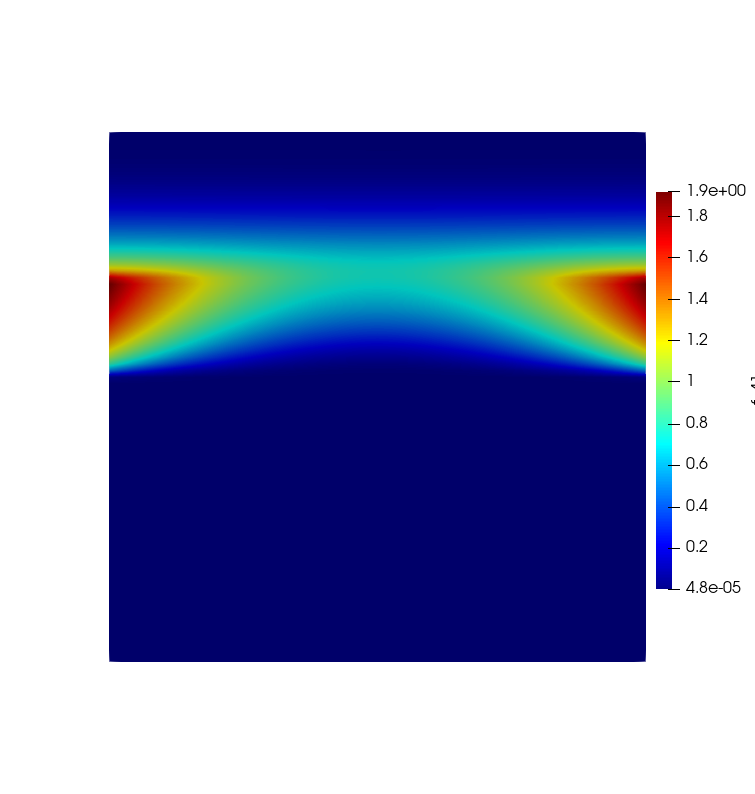
\includegraphics[width=\textwidth]{Figures/testpics/BasicDMA.png}
     \caption{0.08 apart \ce{DMA} after 24 hours}
     \end{subfigure}
     \hspace{1cm}
     \begin{subfigure}[t]{0.35\textwidth}\centering
     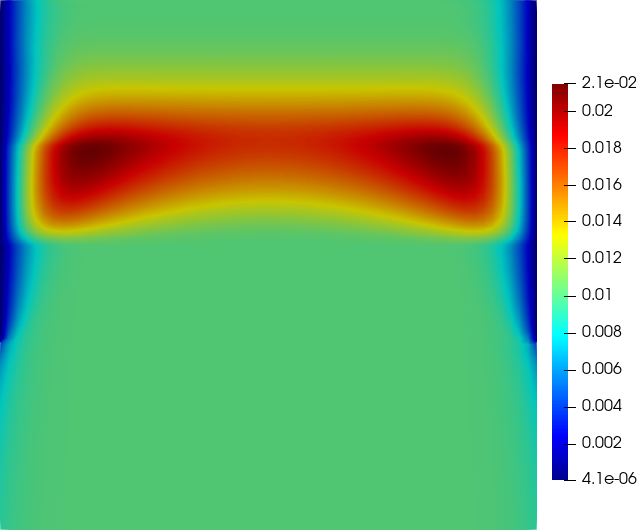
\includegraphics[width=\textwidth]{Figures/testpics/BasicZn.png}
     \caption{0.08 apart \ce{Zn} after 24 hours}
     \end{subfigure}
     \caption{Basic model with parameters from \cite{Ptashnyk-2011} applied to both roots.}
 \end{figure}
 
 As we can see in this base model we observe a good amount of cooperation occurring between the two roots. The DMA exuded from the left has run into that on the right which is causing more \ce{Zn} to be made available to both roots. As the domain is symmetric and the roots close enough that their rhizospheres meet this is as expected. 
%%%%%%%%%%%%%%%%%%%%%%%%%%%%%%%%%%%%%%%%%%%
\subsubsection{Increased distance between roots}
 \begin{figure}
     \centering
     \begin{subfigure}[t]{0.35\textwidth}
     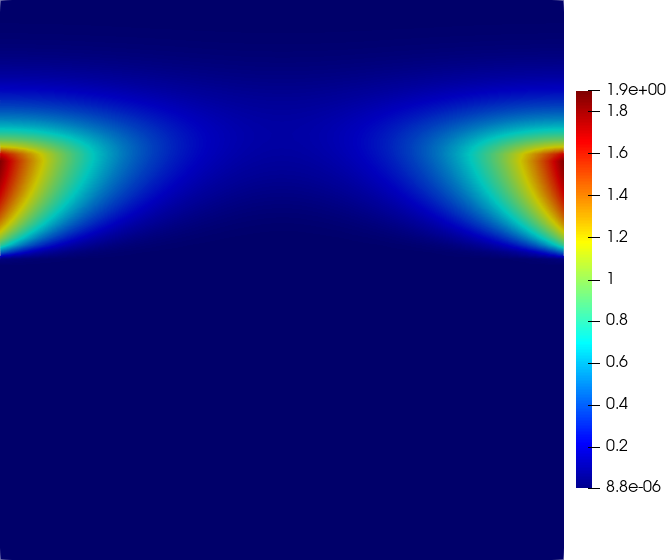
\includegraphics[width=\textwidth]{Figures/testpics/0.15ApartDMA24.png}
     \caption{0.15 dm apart \ce{DMA} after 24 hours}
     \end{subfigure}
     \hspace{1cm}
     \begin{subfigure}[t]{0.35\textwidth}
     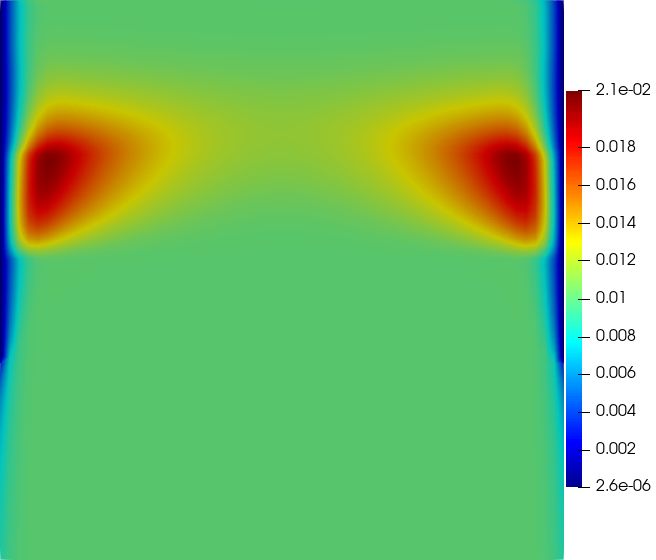
\includegraphics[width=\textwidth]{Figures/testpics/0.15ApartZn24.png}
     \caption{0.15 dm apart \ce{Zn} after 24 hours}
     \end{subfigure}
     \caption{Increased distance between roots, from $0.08$ dm to $0.15$ dm, an increase of 87.5\%.}
 \end{figure}
 Now that the roots have been planted so that their rhizospheres are separated by a large amount of soil area we can observe they have a weaker effect upon each other with the \ce{DMA} graph in the left figure no longer showing any meeting of the exudations from both sides. The \ce{Zn} graph also reflect this, there is no longer a central band of accessible \ce{Zn} within the soil, instead we see two separate zones of increased \ce{Zn} concentration, Perhaps connected very weakly even at this distance as is shown in the very slight band of yellowing within the green area of the soil.
%%%%%%%%%%%%%%%%%%%%%%%%%%%%%%%%%%%%%%%%%%%
\subsubsection{Increased maximum \ce{DMA} exudation}

 \begin{figure}
     \centering
     \begin{subfigure}[t]{0.35\textwidth}
     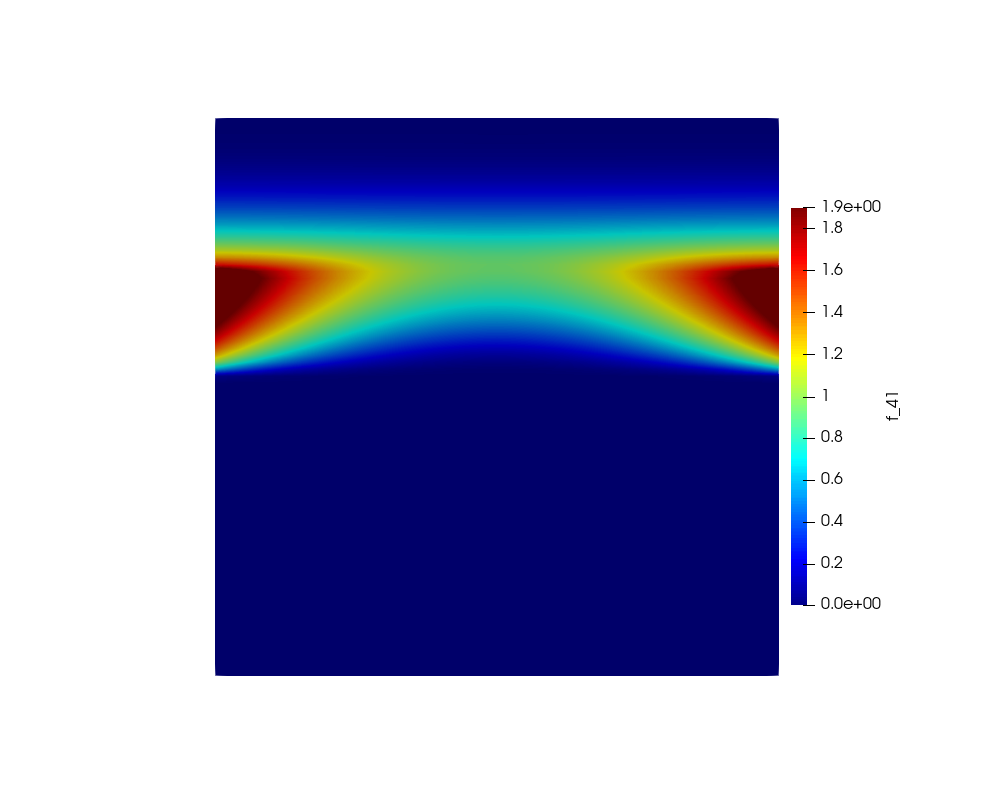
\includegraphics[width=\textwidth]{Figures/testpics/IncreasedBufferDMA24.png} % Hi Liz~
     \caption{0.08 apart, rate of \ce{DMA} exudation increased by $10^{-11}$, \ce{DMA} after 24 hours}
     \end{subfigure}
     \hspace{1cm}
     \begin{subfigure}[t]{0.35\textwidth}
     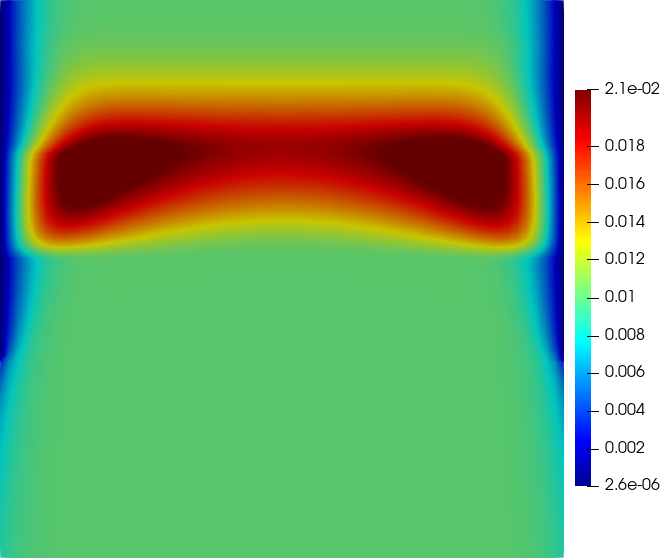
\includegraphics[width=\textwidth]{Figures/testpics/IncreasedBufferZn24.png}
     \caption{0.08 apart, rate of \ce{DMA} exudation increased by $10^{-11}$, \ce{Zn} after 24 hours}
     \end{subfigure}
     \caption{DMA increased}
 \end{figure}
 With a larger exudation of \ce{DMA} by the plant we see, as would be intuitively expected, a larger amount of \ce{Zn} in the soil. The bands we saw in the first plot are larger and more concentrated in these conditions. This suggets that rice plants with a stronger expression of the genes linked with \ce{DMA} exudation may be better at accessing \ce{Zn} in soil and leads us to question whether they would allow an increased distance between plants before this positive cooperation would fade, which we can investigate further.
 
 
%%%%%%%%%%%%%%%%%%%%%%%%%%%%%%%%%%%%%%%%%%%
\subsubsection{Increased distance between plants and maximum \ce{DMA} exudation}

 \begin{figure}
     \centering
     \begin{subfigure}[t]{0.35\textwidth}
     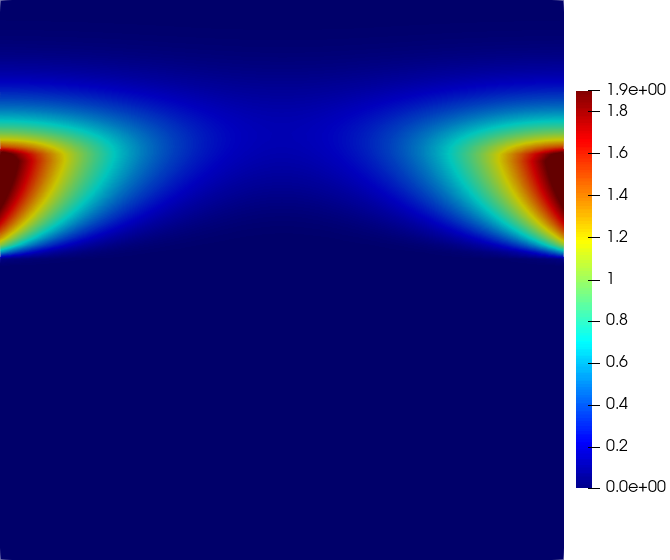
\includegraphics[width=\textwidth]{Figures/testpics/IncreasedBufferAndDistancedDMA24.png}
     \caption{0.15 apart, rate of \ce{DMA} exudation increased by $10^{-11}$, \ce{DMA} after 24 hours}
     \end{subfigure}
     \hspace{1cm}
     \begin{subfigure}[t]{0.35\textwidth}
     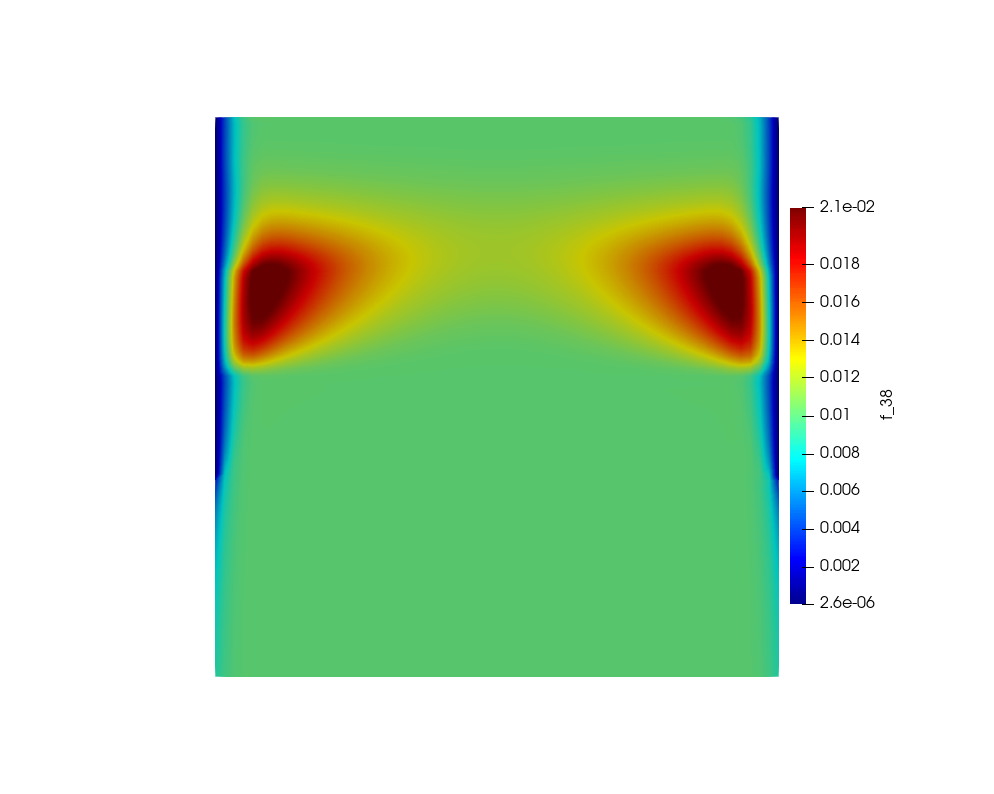
\includegraphics[width=\textwidth]{Figures/testpics/IncreasedBufferAndDistanceZn24.png}
     \caption{0.15 apart, rate of \ce{DMA} exudation increased by $10^{-11}$, \ce{Zn} after 24 hours}
     \end{subfigure}
     \caption{Distance and \ce{DMA} exudation increased}
 \end{figure}
 With increased maximum \ce{DMA} exudation we observe the plants do indeed fare better when spread further apart, in comparison the the basic rice when moved apart this model shows more available \ce{Zn} to each plant. The cooperation still isnt as strong as the basic model when close together so its possible some sensitivity analysis investigating these two parameters would be an interesting thing to consider in future work to determine at which point increased \ce{DMA} stops allowing plant cooperation and at what distance this occurs. This would have to allow for the total amount of \ce{Zn} in the soil as a limiting factor of course, and keep in mind realistic limits on the amount of \ce{DMA} possible for rice plants to exude. 
 
%%%%%%%%%%%%%%%%%%%%%%%%%%%%%%%%%%%%%%%%%%%
 \subsubsection{Increased rate of \ce{Zn} absorption}
 \begin{figure}
     \centering
     \begin{subfigure}[t]{0.35\textwidth}
     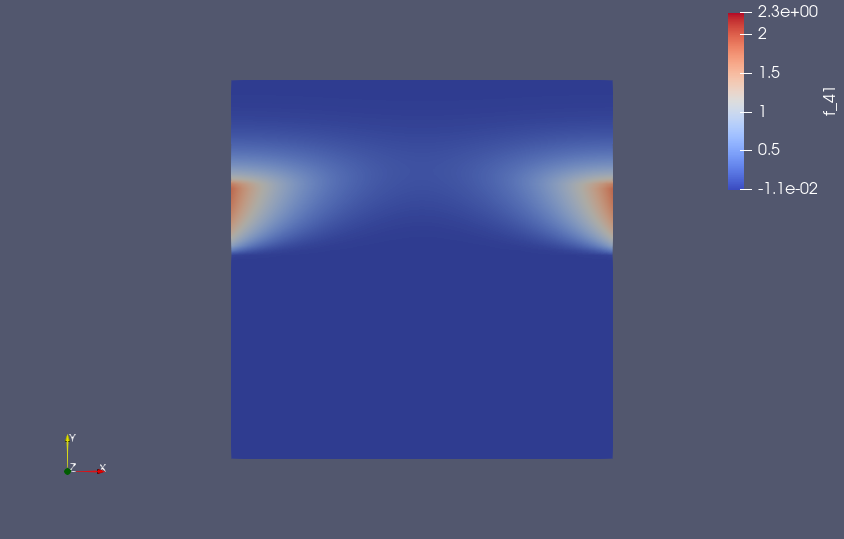
\includegraphics[width=\textwidth]{Figures/testpics/IncreasedZnAbsorbDMA24.png}
     \caption{0.08 apart, rate of \ce{Zn} absorption increased by $0.5e^{-2}$, \ce{DMA} after 24 hours}
     \end{subfigure}
     \hspace{1cm}
     \begin{subfigure}[t]{0.35\textwidth}
     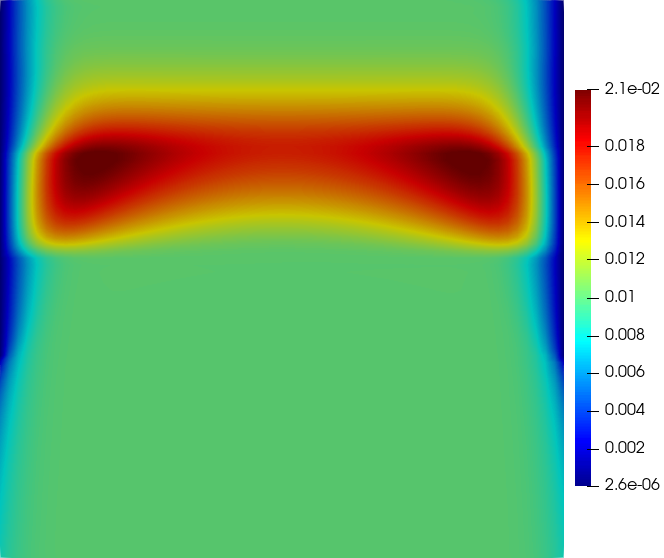
\includegraphics[width=\textwidth]{Figures/testpics/IncreasedZnAbsorbZn24.png}
     \caption{0.08 apart, rate of \ce{Zn} absorption increased by $0.5e^{-2}$, Zn after 24 hours}
     \end{subfigure}
     \caption{Distance and \ce{DMA} exudation increased}
 \end{figure}
If instead we increase the rate of \ce{Zn} absorption by the rice plant we see that these plots remain very similar to our original model. However in this case the plant seems to begin to exude more \ce{DMA} earlier in its growth as we see higher \ce{Zn} concentration closer to the roots surface. \textcolor{red}{Check this later.}


\newpage

% -------------------------------------------------------------------------------

\section{Extended model}
\label{sec:Extension}
We will consider a model where two plants secrete two different exudates that act on a nutrient in the soil which is then absorbed through their roots. We will follow the derivation for a model of one plant described in \cite{Ptashnyk-2011}. The main change is in modelling dynamics of an extra nutrient which results in additional term in the equation for dynamics of $X$ and a new equation for the dynamics of the second exudate.
	
Our domain will be a rectangle with a root of plant that secretes exudate $Y_1$ on the left-hand side, and a root of plant secreting exudate $Y_2$ on the right-hand side. The concentrations of $X$, $Y_1$, and $Y_2$ in the soil solution will be marked by $X_L$, $Y_{L,1}$, and $Y_{L,2}$, while their concentrations in the soil solid in rapid equilibrium with the solution will be $X_S$, $Y_{S,1}$, and $Y_{S,2}$. The conservation equations for $X$, $Y_1$, and $Y_2$ in unit volume of soil are
\begin{align}
	\partial_t(\theta X_L + X_S) &= \nabla \cdot(D_X \nabla X_L - \nu X_L) - g_X, \label{x_1}\\
	\partial_t(\theta Y_{L,1} + Y_{S,1}) &= \nabla \cdot(D_{Y,1} \nabla Y_{L,1} - \nu Y_{L,1}) - g_{Y,1}, \label{y1_1} \\
	\partial_t(\theta Y_{L,2} + Y_{S,2}) &= \nabla \cdot(D_{Y,2} \nabla Y_{L,2} - \nu Y_{L,2}) - g_{Y,2}, \label{y2_1}		
\end{align}
with the involved parameters presented in Table \ref{t:Second-model-params}. Next, we specify the equations for interaction between the nutrients in the solid and in the solution assuming $Y_1$ and $Y_2$ do not interact with each other. This is represented with the following system of ordinary differential equations
\begin{align}
	\partial X_S &= \beta_1 X_L - \beta_2 X_S - \beta_3 X_S Y_{L,1} - \beta_4 X_S Y_{L,2},  \\
	\partial Y_{S,1} &= \gamma_1 Y_{L,1} - \gamma_2 Y_{S,2} - \gamma_3 Y_{S,1} X_L, \\
	\partial Y_{S,2} &= \xi_1 Y_{L,2} - \xi_2 Y_{S,2} - \xi_3 Y_{S,2} X_L,
\end{align}	
where $\beta_1$, $\beta_2$, $\beta_3$, $\beta_4$, $\gamma_1$, $\gamma_2$, $\gamma_3$, $\xi_1$, $\xi_2$, and $\xi_3$ are reaction rate coefficients. At equilibrium we have $\partial_t X_S = \partial_t Y_{S,1} = \partial_t Y_{S,2} = 0$, therefore
\begin{align}
	X_S &= \frac{\beta_1 X_L}{\beta_2 + \beta_3Y_{L,1} + \beta_4 Y_{L,2}}, \label{x_2} \\
	Y_{S,1} &= \frac{\gamma_1 Y_{L,1}}{\gamma_2 + \gamma_3X_L}, \label{y1_2} \\
	Y_{S,2} &= \frac{\xi_1 Y_{L,2}}{\xi_2 + \xi_3X_L}. \label{y2_2}
\end{align}
We differentiate the equations \eqref{x_2}, \eqref{y1_2}, and \eqref{y2_2}, which gives us 
\begin{align}
	\partial_t X_S &= \frac{\beta_1}{\beta_2 + \beta_3 Y_{L,1} + \beta_4 Y_{L,2}} \partial_t X_L - \frac{\beta_1 X_L \beta_3}{(\beta_2 + \beta_3 Y_{L,1} + \beta_4 Y_{L,2})^2} \partial_t Y_{L,1}
	- \frac{\beta_1 X_L \beta_4}{(\beta_2 + \beta_3 Y_{L,1} + \beta_4 Y_{L,2})^2} \partial_t Y_{L,2}, 
	\label{x_3}
	\\
	\partial_t Y_{S,1} &= \frac{\gamma_1}{\gamma_2 + \gamma_3 X_L} \partial_t Y_{L,1} - \frac{\gamma_1 Y_{L,1} \gamma_3}{(\gamma_2 + \gamma_3 X_L)^2} \partial_t X_L, \label{y1_3}
	\\
	\partial_t Y_{S,2} &= \frac{\xi_1}{\xi_2 + \xi_3 X_L} \partial_t Y_{L,2} - \frac{\xi_1 Y_{L,2} \xi_3}{(\xi_2 + \xi_3 X_L)^2} \partial_t X_L. \label{y2_3}
\end{align} 
Combining equations \eqref{x_1} and \eqref{x_3}, \eqref{y1_1} and \eqref{y1_3}, and \eqref{y2_1} and \eqref{y2_3} gives us
\begin{align}
	\begin{split} 
		\left(\theta + \frac{\beta_1}{\beta_2 + \beta_3 Y_{L,1} + \beta_4 Y_{L,2}}\right) \partial_t X_L - \frac{\beta_1 X_L \beta_3}{(\beta_2 + \beta_3 Y_{L,1} + \beta_4 Y_{L,2})^2} \partial_t Y_{L,1} \\
		\qquad
		- \frac{\beta_1 X_L \beta_4}{(\beta_2 + \beta_3 Y_{L,1} + \beta_4 Y_{L,2})^2} \partial_t Y_{L,2} 
		 &= \nabla \cdot(D_X \nabla X_L - \nu X_L) - g_X, 
	\end{split} \label{x_4} 
	\\
	(\theta + \frac{\gamma_1}{\gamma_2 + \gamma_3 X_L}) \partial_t Y_{L,1} - \frac{\gamma_1 Y_{L,1} \gamma_3}{(\gamma_2 + \gamma_3 X_L)^2} \partial_t X_L)  &= \nabla \cdot(D_{Y,1} \nabla Y_{L,1} - \nu Y_{L,1}) - g_{Y,1}, \label{y1_4} 
	\\
	(\theta + \frac{\xi_1}{\xi_2 + \xi_3 X_L}) \partial_t Y_{L,2} - \frac{\xi_1 Y_{L,2} \xi_3}{(\xi_2 + \xi_3 X_L)^2} \partial_t X_L &= \nabla \cdot(D_{Y,2} \nabla Y_{L,2} - \nu Y_{L,2}) - g_{Y,2}. \label{y2_4}	
\end{align}
The set of equations above can be modified by dividing the numerator and denominator of each fraction by an adequate parameter. This way we get the final set of conservation equations in terms of $X_L$, $Y_{L,1}$ and $Y_{L,2}$
\begin{subequations}
\label{eq:extendedsys}
\begin{align}
	\begin{split} 
		&\left( \theta + \frac{b_X}{1 + \kappa_{X,1} b_{X} Y_{L,1} + \kappa_{X,2} b_{X} Y_{L,2}} \right)
		\partial_t X_L - 
		\frac{\kappa_{X,1} b_X^2 X_L}{\big(1 + \kappa_{X,1} b_{X} Y_{L,1} + \kappa_{X,2} b_{X} Y_{L,2} \big)^2} \partial_t Y_{L,1}
		\\
		&\hspace{2.5cm} -
		\frac{\kappa_{X,2} b_X^2 X_L}{\big(1 + \kappa_{X,1} b_{X} Y_{L,1} + \kappa_{X,2} b_{X} Y_{L,2} \big)^2} \partial_t Y_{L,2}
		= \nabla \cdot(D_X \nabla X_L - \nu X_L) - g_X, 
	\end{split} \label{eq:generalised-x_t}
	\\
	&\left(\theta + \frac{b_{Y,1}}{1 + \kappa_{Y,1} b_{Y,1} X_L}\right) \partial_t Y_{L,1}
	- 
	\frac{b_{Y,1}^2 \kappa_{Y,1} Y_{L,1}}{\big(1 + \kappa_{Y,1} b_{Y,1} X_L\big)^2} \partial_t X_L 
	= \nabla \cdot(D_{Y,1} \nabla Y_{L,1} - \nu Y_{L,1}) - g_{Y,1}, \label{eq:generalised-y_1_t}
	\\
	&\left(\theta + \frac{b_{Y,2}}{1 + \kappa_{Y,2} b_{Y,2} X_L}\right) \partial_t Y_{L,2} - \frac{ b_{Y,2}^2 \kappa_{Y,2} Y_{L,2}}{\big(1 + \kappa_{Y,2} b_{Y,2} X_L\big)^2} \partial_t X_L
	= \nabla \cdot(D_{Y,2} \nabla Y_{L,2} - \nu Y_{L,2}) - g_{Y,2}, \label{eq:generalised-y_2_t}
\end{align}
\end{subequations}
where $b_X = \beta_1 / \beta_2$, $b_{Y,1} = \gamma_1 / \gamma_2$, $b_{Y,2} = \xi_1 / \xi_2$, $\kappa_{X,1} = \beta_3 / \beta_1$, $\kappa_{X,2} = \beta_4 / \beta_1$, $\kappa_{Y,1} = \gamma_3 / \gamma_1$, $\kappa_{Y,1} = \xi_3 / \xi_1$ are parameters presented in Table \ref{t:Second-model-params}.
	
	
%%%%%%%%%%%%%%%%%%%%%%%%%%%%%%%%%%%%%%%%%%
\subsection{Boundary conditions}
The following boundary conditions are expanded upon the right-hand side boundary using the conditions from the base model and symmetry of the domain. On the left-hand side of the domain (plant 1) we have
\begin{subequations}
\label{eq:extendedsys_BCs}
	\begin{align}
		D_X \partial_r X_L - \nu X_L &= \alpha_1 X_L &  r&=a, \quad z\in [-L_1, -(L_1 - \delta L_{X, 1})], \label{3eq_BC1} \\
		D_{Y_1} \partial_r Y_{L,1} - \nu Y_{L,1} &= -F_{Y,1} (t) & r&=a, \quad z \in [-L_1, -(L_1 - \delta L_{Y,1, 1})], \label{3eq_BC2}  
	\end{align}
and on the right-hand side of the domain (plant 2) we have
	\begin{align}
		D_X \partial_r X_L - \nu X_L &= -\alpha_2 X_L  & r&=w+a, \quad z \in [-L_2, -(L_2 - \delta L_{X, 2})], \label{3eq_BC3} \\
		D_{Y_2} \partial_r Y_{L,2} - \nu Y_{L,2} &= F_{Y,2} (t) & r&=w+a, \quad z\in [-L_2, -(L_2 - \delta L_{Y,2, 2})]. \label{3eq_BC4} 
	\end{align}
\end{subequations}
Again, we consider zero-flux conditions for the rest of the boundary.

%%%%%%%%%%%%%%%%%%%%%%%%%%%%%%%%%%%%%%%%%%
%%%%%%%%%%%%%%%%%%%%%%%%%%%%%%%%%%%%%%%%%%
\subsection{Simplified system with no exudate-metal interaction}
We consider a simplification of the system of equations \eqref{eq:generalised-x_t} - \eqref{eq:generalised-y_2_t} in a regime where $\kappa_{Y,1} = \kappa_{Y,2} = 0$, i.e., the exudates do not interact with the metal. In this scenario we get the reduced system 
\begin{subequations}
\label{sys-first-extension}
\begin{align}
	\begin{split} 
		&\left( \theta + \frac{b_X}{1 + \kappa_{X,1} b_{X} Y_{L,1} + \kappa_{X,2} b_{X} Y_{L,2}} \right)
			\partial_t X_L - 
			\frac{\kappa_{X,1} b_X^2 X_L}{\big(1 + \kappa_{X,1} b_{X} Y_{L,1} + \kappa_{X,2} b_{X} Y_{L,2} \big)^2} \partial_t Y_{L,1}
			\\
			&\hspace{2.5cm} -
			\frac{\kappa_{X,2} b_X^2 X_L}{\big(1 + \kappa_{X,1} b_{X} Y_{L,1} + \kappa_{X,2} b_{X} Y_{L,2} \big)^2} \partial_t Y_{L,2}
			= \nabla \cdot(D_X \nabla X_L - \nu X_L) - g_X, 
	\end{split} \label{x_fin2} \\
	&(\theta + b_{Y,1}) \partial_t Y_{L,1}   = \nabla \cdot(D_{Y,1} \nabla Y_{L,1} - \nu Y_{L,1}) - g_{Y,1}, \label{y1_fin2} \\
	&(\theta + b_{Y,2}) \partial_t Y_{L,2}  = \nabla \cdot(D_{Y,2} \nabla Y_{L,2} - \nu Y_{L,2}) - g_{Y,2}. \label{y2_fin2}	
\end{align}
\end{subequations}

%%%%%%%%%%%%%%%%%%%%%%%%%%%%%%%%%%%%%%%%%%
%%%%%%%%%%%%%%%%%%%%%%%%%%%%%%%%%%%%%%%%%%
%%%%%%%%%%%%%%%%%%%%%%%%%%%%%%%%%%%%%%%%%%
% \subsection{Boundary conditions}
	
% 	Left-hand side of the domain (plant 1):
% 	\begin{subequations}

% 	\begin{align}
% 		D_X \partial_r X_L - \nu X_L &= \alpha_1 X_L &  r&=a, \quad z\in [L_1 - \delta L_{X, 1},L_1], \label{3eq_BC1} \\
% 		D_{Y_1} \partial_r Y_{L,1} - \nu Y_{L,1} &= -F_{Y,1} (t) & r&=a, \quad z \in [L_1 - \delta L_{Y,1, 1},L_1]. \label{3eq_BC2}  
% 	\end{align}
% 	Right-hand side of the domain (plant 2):
% 	\begin{align}
% 		D_X \partial_r X_L - \nu X_L &= -\alpha_2 X_L  & r&=w+a, \quad z \in [L_2 - \delta L_{X, 2}, L_2], \label{3eq_BC3} \\
% 		D_{Y_2} \partial_r Y_{L,2} - \nu Y_{L,2} &= F_{Y,2} (t) & r&=w+a, \quad z\in [L_2 - \delta L_{Y,2, 2},L_2]. \label{3eq_BC4} 
% 	\end{align}
% \end{subequations}
% Again we consider zero-flux conditions for the rest of the boundary.


\begin{table}[!htb]
\begin{center}
% \caption{Table of parameters and their meanings for the extended model.}
\fontsize{9.5}{7}\selectfont
\setlength{\tabcolsep}{5.pt}
\def\arraystretch{1.5}
\begin{tabular}{ll}
\toprule
    \bf Symbol & \multicolumn{1}{c}{\bf Meaning}
    %
    \\ \midrule
%     $D_X$ & Diffusion of micronutrient $X$ in the soil, $D_X = D_{L,X} \theta f$  \\  
% 	$D_{Y,1}$ &  Diffusion of the PS $Y_1$ in the soil, $D_{Y,1} = D_{L,Y,1} \theta f$  \\   
% 	$D_{Y,2}$ & Diffusion of the PS $Y_2$ in the soil, $D_{Y,2} = D_{L,Y,2} \theta f$\\
    $D_{LX}$ & Diffusion of micronutrient $X$ in free solution \\  
	$D_{LY,1}$ &  Diffusion of exudate $Y_1$ in free solution \\   
	$D_{LY,2}$ & Diffusion of the exudate $Y_2$ in free solution \\
% 	$\nu$ & Water flux\\
	$g_X$ & Function for immobilisation of $X$ \\
	$g_{Y,1}$ & Function for decomposition of $Y_1$ \\
	$g_{Y,2}$ & Function for decomposition of $Y_2$ \\
	$b_X$ & Buffer power of $X$ \\
	$b_{Y,1}$ & Buffer power of $Y_1$ \\
	$b_{Y,2}$ & Buffer power of $Y_2$ \\
	$\kappa_{X,1}$ & $X$ - $Y_1$ interaction coefficient \\
	$\kappa_{X,2}$ & $X$ - $Y_2$ interaction coefficient\\
	$\kappa_{Y,1}$ & $Y_1$ - $X$ interaction coefficient\\
	$\kappa_{Y,2}$ & $Y_2$ - $X$ interaction coefficient\\ 
	$\alpha_1 $ & $X$-absorbing power of root of plant 1 \\
	$\alpha_2 $ & $X$-absorbing power of root of plant 1 \\
	$F_{Y,1} $ & Rate of $Y_1$ exudation from plant 1 \\
	$F_{Y,2} $ & Rate of $Y_2$ exudation from plant 2 \\
	$L_1$ & Length of root of plant 1 at certain time, increases at rate $G_1$ \\
	$L_2$ & Length of root of plant 1 at certain time, increases at rate $G_2$ \\
	$\delta L_{X,1}$ & Length of $X$ uptake zone at plant 1 \\
	$\delta L_{Y,1,1}$ & Length of $Y_1$ secretion zone at plant 1  \\
	$\delta L_{X,2}$ & Length of $X$ uptake zone at plant 2 \\
	$\delta L_{Y,2,2}$ &  Length of $Y_2$ secretion zone at plant 2 \\
	$a$ & Root radius of plant 1 \\
	%$a_2$ & Root radius of plant 2 \\
	$w$ & Distance between the roots \\
\bottomrule
\end{tabular}
\caption{Table of parameters and their meanings for the extended model.
\label{t:Second-model-params}}
\end{center}
\end{table}


%%%%%%%%%%%%%%%%%%%%%%%%%%%%%%%%%%
%%%%%%%%%%%%%%%%%%%%%%%%%%%%%%%%%%
\subsubsection{Variational formulation}

The existence of a solution of system \eqref{sys-first-extension} is presented in Section \ref{sec:Existence}.
To find the variational formulation of the system, we will use a sufficiently smooth test function and then use a density argument for a more general function space. Let's begin supposing that there is a $\mathcal{C}^2 (\bar \Omega)$ solution pair $(X_L,Y_L)$ and multiply the first equation by a $v \in \mathcal{C}^1 (\bar\Omega)$ function and introduce the functions 
\[
    A(Y_{L,1}, Y_{L,2}) := \theta + \frac{b_X}{1 + \kappa_{X,1} b_{X} Y_{L,1} + \kappa_{X,2} b_{X} Y_{L,2}},
    \qquad
    B(X_L, Y_{L,1}, Y_{L,2}) := \frac{\kappa_{X,1} b_X^2 X_L}{\big(1 + \kappa_{X,1} b_{X} Y_{L,1} + \kappa_{X,2} b_{X} Y_{L,2} \big)^2},
\]
and
\[
    C(X_L, Y_{L,1}, Y_{L,2}) := \frac{\kappa_{X,2} b_X^2 X_L}{\big(1 + \kappa_{X,1} b_{X} Y_{L,1} + \kappa_{X,2} b_{X} Y_{L,2} \big)^2}.
\]
This way \eqref{x_fin2} can be written compactly as
\[
	A(Y_{L,1}, Y_{L,2})      \partial_t X_L - 
	B(X_L, Y_{L,1}, Y_{L,2}) \partial_t Y_{L,1} -
	C(X_L, Y_{L,1}, Y_{L,2}) \partial_t Y_{L,2}
	= \nabla \cdot(D_X \nabla X_L - \nu X_L) - g_X.
\]

Now, let us multiply all three differential equations by the test function \(v\), integrate over \(\Omega\), and use Divergence Theorem. This way we get
\begin{subequations}
\begin{align}
    \int\limits_\Omega
    A(Y_{L,1}, Y_{L,2}) \partial_t X_L v &- B(X_L, Y_{L,1}, Y_{L,2}) \partial_t Y_{L,1} v - C(X_L, Y_{L,1}, Y_{L,2}) \partial_t Y_{L,2} v \dif \mu 
    \notag
    \\
    &=
    \int\limits_\Gamma
    (D_X \nabla X_L - \nu X_L) \cdot \vec{n} v
    \dif \sigma
    -\int\limits_\Omega
    (D_X \nabla X_L - \nu X_L) \cdot \nabla v  \dif \mu
    -\int\limits_\Omega g_X v \dif \mu,
    \\
    \int\limits_\Omega (\theta + b_{Y,1}) \partial_t Y_{L,1} v \dif \mu  &=
    \int\limits_\Gamma (D_{Y,1} \nabla Y_{L,1} - \nu Y_{L,1}) \cdot \vec{n} v \dif\sigma
    -\int\limits_\Omega (D_{Y,1} \nabla Y_{L,1} - \nu Y_{L,1}) \cdot \nabla v \dif\mu - \int\limits_\Omega g_{Y,1} v \dif\mu,
    \\
    \int\limits_\Omega (\theta + b_{Y,2}) \partial_t Y_{L,2} v \dif\mu  &= \int\limits_\Gamma (D_{Y,2} \nabla Y_{L,2} - \nu Y_{L,2}) \cdot \vec{n} v \dif\sigma - 
    \int\limits_\Omega (D_{Y,2} \nabla Y_{L,2} - \nu Y_{L,2}) \cdot \nabla v \dif\mu - \int\limits_\Omega g_{Y,2} v \dif\mu;
\end{align}
\end{subequations}
where $\Gamma$ is the boundary of $\Omega$, $\vec{n}$ its normal vector, and $\sigma$ the surface measure on $\Gamma$. 

Observe that due to the zero-flux constraint, we only need to analyse four segments of $\Gamma$. First, for \( r = a\), we have that \(\vec{n} = (-1,0)\), and we define the sets \( \Gamma_{1, X} = \{a\} \times [L_1 - \delta L_{X,1}]\) and 
\( \Gamma_{1, Y} = \{a\} \times [L_1 - \delta L_{Y,1,1}]\). Second, for \(r = w+a\), we have that \(\vec{n} = (1,0)\), and likewise we define \( \Gamma_{2, X} = \{w+a\} \times [L_2 - \delta L_{X,2}]\) and \( \Gamma_{2, Y} = \{w+a\} \times [L_2 - \delta L_{Y,2,2}]\). This way we can split \(\Gamma\) as 
\[ 
    \Gamma = \Gamma_0 \cup \Gamma_{1, X} \cup \Gamma_{1, Y} \cup \Gamma_{2, X} \cup \Gamma_{2,Y},
\]
where \( \Gamma_0 = \Gamma \setminus (\bar{\Gamma}_{1, X} \cup \bar{\Gamma}_{1, Y} \cup \bar{\Gamma}_{2, X} \cup \bar{\Gamma}_{2,Y}) \) is the set with zero flux conditions.
Thence
\begin{subequations}
\label{sys:two-plants-1-weak}
\begin{align}
    \int\limits_\Omega
    A(Y_{L,1}, Y_{L,2}) \partial_t X_L v &- B(X_L, Y_{L,1}, Y_{L,2}) \partial_t Y_{L,1} v - C(X_L, Y_{L,1}, Y_{L,2}) \partial_t Y_{L,2} v \dif \mu 
    \notag
    \\
    &=
    -\int\limits_{\Gamma_{2,X}}  \alpha_2 X_L v \dif \sigma
    - \int\limits_{\Gamma_{1,X}} \alpha_1 X_L v \dif \sigma
    -\int\limits_\Omega
    (D_X \nabla X_L - \nu X_L) \cdot \nabla v  \dif \mu
    -\int\limits_\Omega g_X v \dif \mu,
    \\
    \int\limits_\Omega (\theta + b_{Y,1}) \partial_t Y_{L,1} v \dif \mu  &=
    \int\limits_{\Gamma_{1,Y}} F_{Y,1} v \dif\sigma
    -\int\limits_\Omega (D_{Y,1} \nabla Y_{L,1} - \nu Y_{L,1}) \cdot \nabla v \dif\mu - \int\limits_\Omega g_{Y,1} v \dif\mu,
    \\
    \int\limits_\Omega (\theta + b_{Y,2}) \partial_t Y_{L,2} v \dif\mu  &= \int\limits_{\Gamma_{2,Y}} F_{Y,2} v \dif\sigma - 
    \int\limits_\Omega (D_{Y,2} \nabla Y_{L,2} - \nu Y_{L,2}) \cdot \nabla v \dif\mu - \int\limits_\Omega g_{Y,2} v \dif\mu.
\end{align}
\end{subequations}
Notice that by density, each equation in \eqref{sys:two-plants-1-weak} has to be satisfied for all \(v\in H^1(\Omega)\).


%%%%%%%%%%%%%%%%%%%%%%%%%%%%%%%%%
%%%%%%%%%%%%%%%%%%%%%%%%%%%%%%%%%
\subsubsection{Numerical approximation}

Again we include a simple backward difference scheme for finding solutions of \eqref{sys:two-plants-1-weak}. As before, we will discretise the time domain; then, let the superscript $n$ denote a quantity at time $t_n$, where $n$ is an integer counting time levels; e.g. $X_L^n$ is $X_L$ evaluated at time level $n$. This way we get the following system of discretised equations in time:
\begin{subequations}
\label{sys:two-plants-1-weak-euler}
\begin{align}
    \int\limits_\Omega
    A(Y_{L,1}^{n+1}, Y_{L,2}^{n+1}) (X_L^{n+1} - X_L^n) v &- B(X_L^{n+1}, Y_{L,1}^{n+1}, Y_{L,2}^{n+1}) (Y_{L,1}^{n+1} - Y_{L,1}^n) v 
    \notag
    \\
    &\qquad\quad - C(X_L^{n+1}, Y_{L,1}^{n+1}, Y_{L,2}^{n+1}) (Y_{L,2}^{n+1} - Y_{L,2}^n) v \dif \mu 
    \notag
    \\
    &= -\Delta t
    \int\limits_{\Gamma_{2,X}}  \alpha_2 X_L^{n+1} v \dif \sigma
    - \Delta t \int\limits_{\Gamma_{1,X}} \alpha_1 X_L^{n+1} v \dif \sigma
    \\
    &\qquad\qquad - \Delta t \int\limits_\Omega
    (D_X \nabla X_L^{n+1} - \nu X_L^{n+1}) \cdot \nabla v  \dif \mu
    - \Delta t \int\limits_\Omega g_X^{n+1} v \dif \mu,
    \notag
    \\
    %
    \int\limits_\Omega (\theta + b_{Y,1}) (Y_{L,1}^{n+1} - Y_{L,1}^n) v \dif \mu  &=
    \Delta t \int\limits_{\Gamma_{1,Y}} F_{Y,1} v \dif\sigma
    \notag \\ & \qquad
    - \Delta t \int\limits_\Omega (D_{Y,1} \nabla Y_{L,1}^{n+1} - \nu Y_{L,1}^{n+1}) \cdot \nabla v \dif\mu -  \Delta t \int\limits_\Omega g_{Y,1}^{n+1} v \dif\mu,
    \\
    %
    \int\limits_\Omega (\theta + b_{Y,2}) (Y_{L,2}^{n+1} - Y_{L,2}^n) v \dif\mu  &= \Delta t \int\limits_{\Gamma_{2,Y}} F_{Y,2} v \dif\sigma 
    \notag \\ & \qquad
    - \Delta t 
    \int\limits_\Omega (D_{Y,2} \nabla Y_{L,2}^{n+1} - \nu Y_{L,2}^{n+1}) \cdot \nabla v \dif\mu - \Delta t \int\limits_\Omega g_{Y,2}^{n+1} v \dif\mu.
\end{align}
\end{subequations}
System \eqref{sys:two-plants-1-weak-euler} is to be solved at each level in time \( n\) with initial conditions \( (X_L^0,Y_{L,1}^0, Y_{L,2}^0)\). Notice that the scheme is further applicable for any suitable scaling.




\subsection{Both plants secrete both exudates}
% Previously: plant 1 secreted $Y_1$, plant 2 secreted $Y_2$ - now we improve the boundary conditions so that both plants exude $Y_1$ and $Y_2$: 
We can further extend the model defined in this section so that both plants exude the same two exudates. This change is reflected only in the boundary conditions. On the left-hand side of the domain (plant 1) we add the exudation of $Y_2$,
\begin{subequations}
\label{bounday-two-two}
\begin{align}
	D_X \partial_r X_L - \nu X_L &= \alpha_1 X_L & r&=a, \quad z \in [L_1, L_1 - \delta L_{X,1}] 
	\label{3eq2_BC1} \\
	D_{Y_1} \partial_r Y_{L,1} - \nu Y_{L,1} &= -F_{Y,1,1} (t) & r&=a, \quad z\in  [-L_1,-( L_1 - \delta L_{Y,1, 1} ) ] \label{3eq2_BC2} 
	\\
	D_{Y_2} \partial_r Y_{L,2} - \nu Y_{L,2} &= -F_{Y,2,1} (t) & r&=a, \quad z \in [-L_1, -(L_1 - \delta L_{Y,2, 1})] 
	\label{3eq2_BC3} 
\end{align}
and on the right-hand side of the domain (plant 2) we add the exudation of $Y_1$,
\begin{align}
	D_X \partial_r X_L - \nu X_L &= -\alpha_2 X_L & r&=w+a, \quad z \in [-L_2, -(L_2 - \delta L_{X, 2})], \label{3eq2_BC4} \\
	D_{Y_1} \partial_r Y_{L,1} - \nu Y_{L,1} &= F_{Y,1,2} (t) & r&=w+a, \quad z \in [-L_2, -(L_2 - \delta L_{Y,1, 2})], \label{3eq2_BC5} \\
	D_{Y_2} \partial_r Y_{L,2} - \nu Y_{L,2} &= F_{Y,2,2} (t) & r&=w+a, \quad z \in [-L_2, -(L_2 - \delta L_{Y,2, 2})]. \label{3eq2_BC6} 
\end{align}
\end{subequations}

For our simulations we assume that both exudates at both plants are secreted 2cm behind the root tip. The exudation rates and secretion zone parameters are explained in Table \ref{t:Boundary-additional-parameters} and the situation in the domain is shown in Figure \ref{fig:2roots-b}.

	
\begin{table}[!htb]
\begin{center}
% \caption{Exudation rates.}
\fontsize{9.5}{7}\selectfont
\setlength{\tabcolsep}{5.pt}
\def\arraystretch{1.5}
\begin{tabular}{ll}
\toprule
    \bf Symbol & \multicolumn{1}{c}{\bf Meaning}
    %
    \\ \midrule
	$\delta L_{Y,1,1}$ & Length of $Y_1$ secretion zone at plant 1  \\
	$\delta L_{Y,2,1}$ & Length of $Y_2$ secretion zone at plant 1  \\
	$\delta L_{Y,1,2}$ &  Length of $Y_1$ secretion zone at plant 2 \\
	$\delta L_{Y,2,2}$ &  Length of $Y_2$ secretion zone at plant 2 \\
    $F_{Y,1,1} $ & Rate of $Y_1$ exudation from plant 1 \\
	$F_{Y,2,1} $ & Rate of $Y_2$ exudation from plant 1 \\
	$F_{Y,1,2} $ & Rate of $Y_1$ exudation from plant 2 \\
	$F_{Y,2,2} $ & Rate of $Y_2$ exudation from plant 2 \\
\bottomrule
\end{tabular}
\caption{Additional parameters emerging from the boundary conditions when both plants exude both parameters.
\label{t:Boundary-additional-parameters}}
\end{center}
\end{table}

\begin{figure}[!htb]
    \centering
    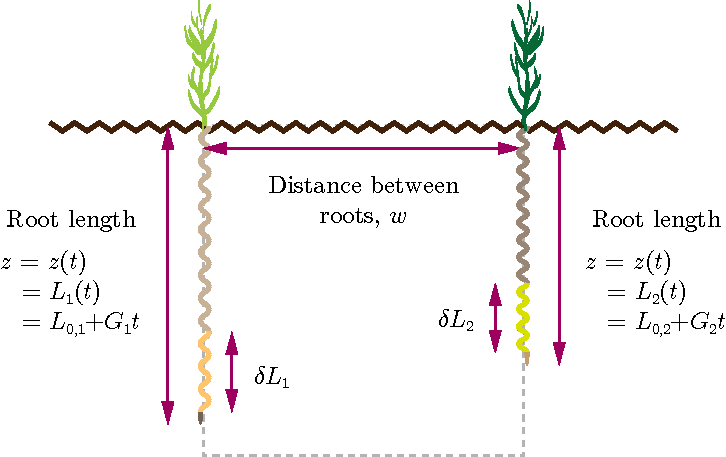
\includegraphics[scale=0.7]{Figures/Third-plot.pdf}
    \caption{Sketch of the domain for system with two plants secreting two exudates.}
    \label{fig:2roots-b}
\end{figure}

The existence of a solution is also contemplated in Section \ref{sec:Existence}.
The resulting variational formulation is 
\begin{subequations}
\label{sys:two-plants-2-weak}
\begin{align}
    \int\limits_\Omega
    A(Y_{L,1}, Y_{L,2}) \partial_t X_L v &- B(X_L, Y_{L,1}, Y_{L,2}) \partial_t Y_{L,1} v - C(X_L, Y_{L,1}, Y_{L,2}) \partial_t Y_{L,2} v \dif \mu 
    \notag
    \\
    &=
    - \int\limits_{\Gamma_{2,X}}  \alpha_2 X_L v \dif \sigma
    - \int\limits_{\Gamma_{1,X}} \alpha_1 X_L v \dif \sigma
    -\int\limits_\Omega
    (D_X \nabla X_L - \nu X_L) \cdot \nabla v  \dif \mu
    -\int\limits_\Omega g_X v \dif \mu,
    \\
    %
    \int\limits_\Omega (\theta + b_{Y,1}) \partial_t Y_{L,1} v \dif \mu  &=
    \int\limits_{\Gamma_{1,1,Y}} F_{Y,1,1} v \dif\sigma
    + \int\limits_{\Gamma_{1,2,Y}} F_{Y,1,2} v \dif\sigma
    -\int\limits_\Omega (D_{Y,1} \nabla Y_{L,1} - \nu Y_{L,1}) \cdot \nabla v \dif\mu - \int\limits_\Omega g_{Y,1} v \dif\mu,
    %
    \\
    \int\limits_\Omega (\theta + b_{Y,2}) \partial_t Y_{L,2} v \dif\mu  &=
    \int\limits_{\Gamma_{2,1,Y}} F_{Y,2,1} v \dif\sigma
    +\int\limits_{\Gamma_{2,2,Y}} F_{Y,2,2} v \dif\sigma - 
    \int\limits_\Omega (D_{Y,2} \nabla Y_{L,2} - \nu Y_{L,2}) \cdot \nabla v \dif\mu - \int\limits_\Omega g_{Y,2} v \dif\mu.
\end{align}
\end{subequations}
Here the sub subsets of \(\Gamma\) are defined implicitly by conditions \eqref{bounday-two-two}.

The discretisation of \eqref{sys:two-plants-2-weak} is similar to the one of \eqref{sys:two-plants-1-weak}. Again, its non-dimensionalisation follows a similar scheme.








%\newpage
%%%%%%%%%%%%%%%%%%%%%%%%%%%%%%%%%%%%%%%%%
%%%%%%%%%%%%%%%%%%%%%%%%%%%%%%%%%%%%%%%%%
\subsection{Non-dimensionalisation}

Similarly as we did in Section \ref{2-Base-Scaling}, 
we will scale the variables of the model appropriately. Again, we introduce the following relations
\[
    r = \varepsilon_r \hat{r} + a,
    \qquad
    z = \varepsilon_z \hat{z},
    \qquad
    t = \varepsilon_t \hat{t},
    \qquad
    X_L = \varepsilon_x \hat{x},
    \qquad
    Y_{L,1} = \varepsilon_{1,y} \hat{y}_1,
    \qquad
    Y_{L,2} = \varepsilon_{2,y} \hat{y}_2;
\]
where \( \varepsilon_r, \varepsilon_z, \varepsilon_t, \varepsilon_x, \varepsilon_{1,y}\), and \(\varepsilon_{2,y}\) are scaling constants to be determined, and \(\hat{r}, \hat z, \hat t, \hat x, \hat y_1\), and \(\hat y_2\) are non-dimensional variables.
Again we get the relations \(X_L(r,z) = \varepsilon_x \hat{x} (\varepsilon_r \hat r + a, \varepsilon_z \hat z) = \varepsilon_x \hat{x} \big( \varepsilon_r^{-1} (r-a) , \varepsilon_z^{-1} z\big) \), \(Y_{L,1} (r,z) = \varepsilon_{1,y} \hat{y}_1 \big( \varepsilon_r^{-1} (r-a), \varepsilon_z^{-1} z \big)\), and \(Y_{L,2} (r,z) = \varepsilon_{2,y} \hat{y}_2 \big( \varepsilon_r^{-1} (r-a), \varepsilon_z^{-1} z \big)\). Again the gradient operator is also scaled as
\[
    \nabla X_L =
    \begin{pmatrix}
        \nicefrac{1}{\varepsilon_r} & 0 \\
        0 & \nicefrac{1}{\varepsilon_z}
    \end{pmatrix}
    \hat{\nabla} \varepsilon_x \hat{x},
    \qquad \text{with} \qquad
    \hat{\nabla} = 
    \begin{pmatrix}
        \pd{ }{\hat r}
        &
        \pd{ }{\hat z}
    \end{pmatrix}^\top .
\]
For ease of presentation, we will separate the derivation into two parts. First, we will find the non-dimensionalised version of the differential equations. Here the choice of the scaling will not be explicit. This changes in the second part, where we present a scaled version of the boundary and initial conditions.

%%%%%%%%%%%%%%%%%%%%%
%%%%%%%%%%%%%%%%%%%%%
%%%%%%%%%%%%%%%%%%%%%
\subsubsection{Scaled differential equations}

The scaled equations can be found following the same steps as before. First consider the quantities
\begin{subequations}
\label{eq:generalised-x_t-parts}
\begin{align}
    \left( \theta + \frac{b_X}{1 + \kappa_{X,1} b_{X} Y_{L,1} + \kappa_{X,2} b_{X} Y_{L,2}} \right) \partial_t X_L &= \frac{\varepsilon_x}{\varepsilon_t} \left( \theta + \frac{b_X}{1 + \varepsilon_{1,y} \kappa_{X,1} b_{X} \hat{y}_1 + \varepsilon_{2,y} \kappa_{X,2} b_{X} \hat{y}_2 } \right)  \pd{\hat{x}}{\hat{t}}
    \\
    \frac{\kappa_{X,1} b_X^2 X_L}{\big(1 + \kappa_{X,1} b_{X} Y_{L,1} + \kappa_{X,2} b_{X} Y_{L,2} \big)^2} \partial_t Y_{L,1} 
    &=
    \frac{\varepsilon_x}{\varepsilon_t} \frac{\varepsilon_{1,y} \kappa_{X,1} b_X^2 \hat{x}}{\big(1+ \varepsilon_{1,y} \kappa_{X,1} b_X \hat{y}_1 + \varepsilon_{2,y} \kappa_{X,2} b_X \hat{y}_2 \big)^2} \pd{\hat y_1}{\hat t}
    \\
    \frac{ \kappa_{X,2} b_X^2 X_L }{\big(1 + \kappa_{X,1} b_X Y_{L,1} + \kappa_{X,2} b_X Y_{L,2}\big)^2} \partial_t Y_{L,2}
    &=
    \frac{\varepsilon_x}{\varepsilon_t} \frac{\varepsilon_{2,y} \kappa_{X,2} b_X^2 \hat{x}}{\big(1+ \varepsilon_{1,y} \kappa_{X,1} b_X \hat{y}_1 + \varepsilon_{2,y} \kappa_{X,2} b_X \hat{y}_2 \big)^2} \pd{\hat y_2}{\hat t}
\end{align}
\end{subequations}

We know that a linear combination of these forms \eqref{eq:generalised-x_t}, from where the term \(\nabla \cdot (D_X \nabla X_L - \nu X_L)\) follows \eqref{eq:divergence-non-dimen-x}.
Proceed to define the scaled constants and vector
\[
    \hat{\kappa}_{X,1} = \varepsilon_{1,y} \kappa_{X,1},
    \qquad
    \hat{\kappa}_{X,2} = \varepsilon_{2,y} \kappa_{X,2},
    \qquad
    \hat{\nu} = 
    \begin{pmatrix}   \hat{\nu}_r    &    \hat{\nu}_z    \end{pmatrix}^\top
    =
    \nu \varepsilon_t
    \begin{pmatrix}    {\varepsilon_r}^{-1}    &    {\varepsilon_z}^{-1}
    \end{pmatrix}^\top ,
\]
define the matrix
\[
    \hat{D}_x = 
    \begin{pmatrix}
         \hat{D}_{X,r} & 0 
         \\
        0 &  \hat{D}_{X,z}
    \end{pmatrix}
    =
    D_X \varepsilon_t
    \begin{pmatrix}
         \varepsilon_r^{-2} & 0 
         \\
        0 &  \varepsilon_z^{-2}
    \end{pmatrix}
    ,
\]
and then define the non-dimensionalised quantity \( \hat{g}_X = \nicefrac{\varepsilon_t}{\varepsilon_x} g_X\). This way we get from \eqref{eq:generalised-x_t-parts} that
\begin{equation}
\begin{aligned}
    \left( \theta + \frac{b_X}{1 + \hat{\kappa}_{X,1} b_{X} \hat{y}_1 + \hat{\kappa}_{X,2} b_{X} \hat{y}_2 } \right)  \pd{\hat{x}}{\hat{t}}
    &
    -\frac{\hat{\kappa}_{X,1} b_X^2 \hat{x}}{\big(1+ \hat{\kappa}_{X,1} b_X \hat{y}_1 + \hat{\kappa}_{X,2} b_X \hat{y}_2 \big)^2} \pd{\hat y_1}{\hat t}
    \\
    &\,\,
    -\frac{\hat{\kappa}_{X,2} b_X^2 \hat{x}}{\big(1+ \hat{\kappa}_{X,1} b_X \hat{y}_1 + \hat{\kappa}_{X,2} b_X \hat{y}_2 \big)^2} \pd{\hat y_2}{\hat t}
    =
    \hat{\nabla}
    \cdot
    \left( 
        \hat{D}_x \hat{\nabla} \hat{x} - \hat{x} \hat{\nu}
    \right)
    - \hat{g}_X.
\end{aligned}
\end{equation}

Similarly, for \eqref{eq:generalised-y_1_t}, we first get the relations
\begin{subequations}
\label{eq:generalised-y_1_t-parts}
\begin{align}
    \left(\theta + \frac{b_{Y,1}}{1 + \kappa_{Y,1} b_{Y,1} X_L}\right) \partial_t Y_{L,1} 
    &= 
    \frac{\varepsilon_{1,y}}{\varepsilon_t} \left( \theta + \frac{b_{Y,1}}{1 + \varepsilon_{x} \kappa_{Y,1} b_{Y,1} \hat{x} } \right)  \pd{\hat{y}_1}{\hat{t}}
    \\
    \frac{ \kappa_{Y,1} b_{Y,1}^2 Y_{L,1}}{\big(1 + \kappa_{Y,1} b_{Y,1} X_L\big)^2} \partial_t X_L
    &=
    \frac{\varepsilon_{1,y}}{\varepsilon_t}
    \frac{ \varepsilon_x  \kappa_{Y,1} b_{Y,1}^2 \hat{y}_{1}}{\big(1 + \varepsilon_x \kappa_{Y,1} b_{Y,1} \hat{x} \big)^2}
    \pd{\hat{x}}{\hat{t}}.
\end{align}
\end{subequations}
Now define
\[
    \hat{\kappa}_{Y,1} = \varepsilon_{x} \kappa_{Y,1},
    \qquad
    \hat{D}_{y,1} = 
    \begin{pmatrix}
         \hat{D}_{Y,1,r} & 0 
         \\
        0 &  \hat{D}_{Y,1,z}
    \end{pmatrix}
    =
    D_{Y,1} \varepsilon_t
    \begin{pmatrix}
         \varepsilon_r^{-2} & 0 
         \\
        0 &  \varepsilon_z^{-2}
    \end{pmatrix},
    \qquad\text{and}\qquad
    \hat{g}_{y,1} = \frac{\varepsilon_t}{\varepsilon_{1,y}} g_{Y,1}
\]
to get from \eqref{eq:generalised-y_1_t-parts} that
\begin{equation}
    \left( \theta + \frac{b_{Y,1}}{1 + \hat{\kappa}_{Y,1} b_{Y,1} \hat{x} } \right)  \pd{\hat{y}_1}{\hat{t}}
    -
    \frac{ \hat{\kappa}_{Y,1} b_{Y,1}^2 \hat{y}_{1}}{\big(1 + \hat{\kappa}_{Y,1} b_{Y,1} \hat{x} \big)^2}
    \pd{\hat{x}}{\hat{t}}
    = \hat{\nabla} \cdot (\hat{D}_{y,1} \hat{y}_1 - \hat{y}_1 \hat{\nu}) - \hat{g}_{y,1}.
\end{equation}




Finally, for \eqref{eq:generalised-y_2_t} define
\[
    \hat{\kappa}_{Y,2} = \varepsilon_{x} \kappa_{Y,2},
    \qquad
    \hat{D}_{y,2} = 
    \begin{pmatrix}
         \hat{D}_{Y,2,r} & 0 
         \\
        0 &  \hat{D}_{Y,2,z}
    \end{pmatrix}
    =
    D_{Y,2} \varepsilon_t
    \begin{pmatrix}
         \varepsilon_r^{-2} & 0 
         \\
        0 &  \varepsilon_z^{-2}
    \end{pmatrix},
    \qquad\text{and}\qquad
    \hat{g}_{y,2} = \frac{\varepsilon_t}{\varepsilon_{2,y}} g_{Y,2},
\]
from which we get
\begin{equation}
    \left(\theta + \frac{b_{Y,2}}{1 + \hat{\kappa}_{Y,2} b_{Y,2} \hat{x}}\right) \pd{\hat{y}_2}{\hat{t}}
    - 
    \frac{ b_{Y,2}^2 \hat{\kappa}_{Y,2} \hat{y}_2 }{\big(1 + \hat{\kappa}_{Y,2} b_{Y,2} \hat{x} \big)^2} \pd{\hat{x}}{\hat{t}} 
    = 
    \hat{\nabla} \cdot(\hat{D}_{y,2} \hat{\nabla} \hat{y}_{2} - \hat{y}_2 \hat{\nu}  ) - \hat{g}_{y,2}.
\end{equation}



%%%%%%%%%%%%%%%%%%%%%
\subsubsection{Scaled boundary and initial conditions}

The choice of the scaling parameters come from the boundary conditions. 



Here we will present the choice and development for the secretion of two exudates. The treatment is similar for the secretion of one. 

Again, the derivation is straightforward from the base model. First, we note that for \(X_L\) we get, for one side of the boundary, that
\[
    D_X \partial_r X_L - \nu X_L = 
    \frac{\varepsilon_r^2}{\varepsilon_t} \hat{D}_{X,r} \frac{\varepsilon_x}{\varepsilon_r} \pd{\hat{x}}{\hat{r}} - \frac{\varepsilon_r}{\varepsilon_t} \hat{\nu}_r \varepsilon_x \hat{x} = \frac{\varepsilon_r \varepsilon_x}{\varepsilon_t} \hat{\alpha}_1 \hat{x}
    \qquad \text{at } r = a = a + \varepsilon_r \hat{r}, \quad \varepsilon_z \hat{z} \in [L_1 - \delta L_{X,1}, L_1],
\]
or equivalently
\begin{subequations}
\begin{equation}
    \hat{D}_{X,r} \pd{\hat{x}}{\hat{r}} - \hat{\nu}_r \hat{x} = \hat{\alpha}_1 \hat{x}
    \qquad \text{at } \hat{r} = 0, \quad \hat{z} \in [\hat{L}_1 - \delta \hat{L}_{x,1}, \hat{L}_1];
\end{equation}
where we require \( \alpha_1 = \nicefrac{\varepsilon_r}{\varepsilon_t} \hat{\alpha}_1\), \( \hat{L}_1 = \varepsilon_z^{-1} L_1\), and \( \delta\hat{L}_{x,1} = \varepsilon_z^{-1} \delta L_{X,1}\). Similarly, the other side of the boundary follows
\begin{equation}
    \hat{D}_{X,r} \pd{\hat{x}}{\hat{r}} - \hat{\nu}_r \hat{x} = -\hat{\alpha}_2 \hat{x}
    \qquad \text{at } \hat{r} = 1, \quad \hat{z} \in [\hat{L}_2 - \delta \hat{L}_{x,2}, \hat{L}_2];
\end{equation}
where we have selected \( \varepsilon_r = w\), and a proper selection of constants as in the previous line.

The relationships for \(Y_{L,1}\) and \(Y_{L,2}\) are similar:
\begin{align}
    \hat{D}_{Y,1,r} \pd{\hat{y}_1}{\hat{r}} - \hat{\nu}_r \hat{y}_1 &= -\hat{F}_{1,1}(t)
    &
    \text{at } \hat{r} &= 0, \quad \hat{z} \in [\hat{L}_1 - \delta \hat{L}_{y,1,1}, \hat{L}_1],
    \\
    \hat{D}_{Y,2,r} \pd{\hat{y}_2}{\hat{r}} - \hat{\nu}_r \hat{y}_2 &= -\hat{F}_{2,1}(t)
    &
    \text{at } \hat{r} &= 0, \quad \hat{z} \in [\hat{L}_1 - \delta \hat{L}_{y,2,1}, \hat{L}_1],
    \\
    \hat{D}_{Y,1,r} \pd{\hat{y}_1}{\hat{r}} - \hat{\nu}_r \hat{y}_1 &= \hat{F}_{1,2}(t)
    &\text{at } \hat{r} &= 1, \quad \hat{z} \in [\hat{L}_2 - \delta \hat{L}_{y,1,2}, \hat{L}_2],
    \\
    \hat{D}_{Y,2,r} \pd{\hat{y}_2}{\hat{r}} - \hat{\nu}_r \hat{y}_2 &= \hat{F}_{2,2}(t)
    &\text{at } \hat{r} &= 1, \quad \hat{z} \in [\hat{L}_2 - \delta \hat{L}_{y,2,2}, \hat{L}_2];
\end{align}
\end{subequations}
where appropriate quantities are selected. For instance \( \hat{F}_{1,1} = \frac{\varepsilon_t}{\varepsilon_r \varepsilon_{1,y}} F_{Y,1,1} \).

For the other scaling parameters, notice that if we again pick \( \varepsilon_z = L_{t_{\max}}\), again \(\hat z \) will be in the range \( [0,1]\) (or \([0,-1]\) when growth is modelled downwards). 
This choice implies that \( \max_t\{|\hat{L}_1|,|\hat{L}_2|\}\) should be \(1\), where we have
\begin{align}
    \hat{L}_1 &= \hat{L}_1(\hat t) = \frac{1}{\varepsilon_z} ( L_{1,0} + G_1 \varepsilon_t \hat t )
    = \hat{L}_{1,0} + \hat{G}_1 \hat t,
    \qquad 
    \hat{L}_{1,0} = \varepsilon^{-1}_z L_{1,0},
    \qquad
    \hat{G}_1 = \varepsilon_t \varepsilon_z^{-1} G_1,
    \\
    \hat{L}_2 &= \hat{L}_2(\hat t) = \frac{1}{\varepsilon_z} ( L_{2,0} + G_2 \varepsilon_t \hat t )
    = \hat{L}_{2,0} + \hat{G}_2 \hat t,
    \qquad 
    \hat{L}_{2,0} = \varepsilon^{-1}_z L_{2,0},
    \qquad
    \hat{G}_2 = \varepsilon_t \varepsilon_z^{-1} G_2;
\end{align}
and we can further select \( \varepsilon_t = t_{\max}\) to finally have \( \hat t\) in the range \( [0,1]\). As a result, we have selected scaling parameters such that the system of partial differential equations is defined in either \( [0,1]^3\) or \([0,1]\times [0,-1] \times [0,1]\).
%
Lastly, the initial conditions are scaled as \( (\hat{x}_0,\hat{y}_{1,0},\hat{y}_{2,0} ) = (\varepsilon_x^{-1} X^0_L, \varepsilon_{1,y}^{-1} Y^0_{L,1}, \varepsilon_{2,y}^{-1} Y^0_{L,2}) \). 


Observe that again we can use parameters \(\varepsilon_x\), \(\varepsilon_{1,y}\), and \(\varepsilon_{2,y}\) to calibrate the effects of \( \hat{x}\) and \(\hat{y}\) in all of the nonlinear terms in the above equations.

%%%%%%%%%%%%%%%%%%%%%%%%%%%%%%%%%%%%%%%%%%%%%%%%%%%%%%%%%%%%%%%%%%%%%%%%%%%
%%%%%%%%%%%%%%%%%%%%%%%%%%%%%%%%%%%%%%%%%%%%%%%%%%%%%%%%%%%%%%%%%%%%%%%%%%%
%%%%%%%%%%%%%%%%%%%%%%%%%%%%%%%%%%%%%%%%%%%%%%%%%%%%%%%%%%%%%%%%%%%%%%%%%%%

\section{Results of the extended model}
\label{sec:Results_Extension}


In order to solve the system numerically, we will use the open-source computing platform FEniCS, a framework for PDE modeling, continuum mechanics, and physics simulations \cite{fenics}. FEniCS enables users to translate the mathematical problem into Python code and solve it efficiently using the finite element method. The main benefits of this software are that the code is close to the mathematical formulation and that the implementation of the model does not get much more difficult as the complexity of the model increases.
% \begin{itemize}
%     \item mention negative values at some point in the simulation (numeric errors?)
% \end{itemize}

\textcolor{red}{Explain how this is implemented in the code (linearisation, first solve for Y1, Y2, then for X), simplifying assumptions?}


\subsection{Parameters for barley-tobacco combination}
In this section, we discuss the selection of parameters in Table \ref{t:Second-model-params} to model the dynamics between exudates of barley and tobacco plants and \ce{P} in the soil.

\begin{table}[!htb]
\begin{center}
% \caption{Table of parameters with their meanings and values, plant 1 (LHS) is barley, plant 2 (RHS) is tobacco, component $X$ is phosphate, $Y_1$ is phytase, and $Y_2$ is citrate.}
\fontsize{9.5}{7}\selectfont
\setlength{\tabcolsep}{5.pt}
\def\arraystretch{1.5}
\begin{tabular}{lll}
\toprule
    \bf Symbol & \multicolumn{1}{l}{\bf Meaning} & \bf Value
    %
    \\ \midrule
    $\theta$ & Solution volume fraction & 0.2 -- 0.3 dm$^3$ $dm^{-3}$ \\
    $f$ & Diffusion impedance factor & 0.5 \\ 
    $\rho$ & Soil bulk density & 1.2 kg dm$^{-3}$ \\
    $D_{LX} $ & Diffusion coefficient of phosphate in free solution & $7-9 \times 10^{-8}$ dm$^2$ s$^{-1}$ \\  
	$D_{LY,1}$ &  Diffusion of phytase in free solution & $3.5 - 4.5 \times 10^{-8}$ dm$^2$ s$^{-1}$ \\   
	$D_{LY,2}$ & Diffusion of citrate in free solution & $2.1 \times 10^{-8}$ dm$^2$ s$^{-1}$ \\
	$\nu$ & Water flux & $1 \times 10^{-6}$ dm s$^{-1}$\\
	$g_X$ & Function for phosphate immobilisation & 0 \\
	$g_{Y,1}$ & Function for phytase decomposition & 0 \\
	$g_{Y,2}$ & Function for citrate decomposition & $\frac{\rho V_{max} Y_{L,2} }{K_M + Y_{L,2} }$ where $V_{max} = 0$ or $V_{max} = 2.5 \times 10^{-9}$ mol kg$^{-1}$ s$^{-1}$, \\
	 & & $K_M=10^{-8}$ M \\
	$b_X$ & Phosphate buffer power & 300 -- 2200 \\
	$b_{Y,1}$ & Phytase buffer power & 1 \\
	$b_{Y,2}$ & Citrate buffer power & 1 \\
	$\kappa_{X,1}$ & Phosphate - phytase interaction coefficient & 18.43 dm$^3$ mol$^{-1}$ \\
	$\kappa_{X,2}$ & Phosphate - citrate interaction coefficient & $92.16$ dm$^3$ mol$^{-1}$ \\
	$\kappa_{Y,1}$ & Phytase - phosphate interaction coefficient & 0 \\
	$\kappa_{Y,2}$ & Citrate - phosphate interaction coefficient & 0 \\ 
	$\alpha_1 $ & Phosphate absorbing power of root of barley & $5.6 \times 10^{-3}$ dm s$^{-1}$\\
	$\alpha_2 $ & Phosphate absorbing power of root of tobacco & $5.6 \times 10^{-3}$ dm s$^{-1}$\\
	$F_{Y,1,1} $ & Rate of phytase exudation in barley & $2.466 \times 10^{-11} - 2.503 \times 10^{-10}$  mol dm$^{-2}$ s$^{-1}$ \\
	$F_{Y,2,1} $ & Rate of citrate exudation in barley & $1.097 \times 10^{-12} - 1.006 \times 10^{-9}$ mol dm$^{-2}$ s$^{-1}$ \\
	$F_{Y,1,2} $ & Rate of phytase exudation in tobacco &  $1.316 \times 10^{-6}$ mol dm$^{-2}$ s$^{-1}$ \\
	$F_{Y,2,2} $ & Rate of citrate exudation in tobacco &  $2.722 \times 10^{-6}$ mol dm$^{-2}$ s$^{-1}$ \\
	$L_1$ & Barley root length & increases at rate $G_1 = 0.1728$ dm day$^{-1}$ \\
	$L_2$ & Tobacco root length & increases at rate $G_2 = 0.2$ dm day$^{-1}$\\
	$\delta L_{X,1}$ & Length of phosphate uptake zone at barley & $L_1$\\
	$\delta L_{Y,1,1}$ & Length of phytase secretion zone at barley & 0.2 dm \\
	$\delta L_{Y,1,2}$ & Length of citrate secretion zone at barley & 0.2 dm\\
	$\delta L_{X,2}$ & Length of phosphate uptake zone at tobacco & $L_2$ \\
	$\delta L_{Y,1,2}$ &  Length of phytase secretion zone at tobacco & 0.2 dm \\
	$\delta L_{Y,2,2}$ &  Length of citrate secretion zone at tobacco & 0.2 dm \\
	$a$ & Root radius of barley & 0.005 dm \\
	$w$ & Distance between the roots & varied \\
\bottomrule

\end{tabular}
% \label{t:Second-model-params}
\caption{Table of parameters with their meanings and values used for numerical experiments in this section, plant 1 (LHS) is barley, plant 2 (RHS) is tobacco, component $X$ is phosphate, $Y_1$ is phytase, and $Y_2$ is citrate. \label{t:Second-model-params}
}
\end{center}

\end{table}

\subsubsection{Soil parameters}
We choose the water content in soil $\theta$ to be in the range $0.2$ to $0.3$ which should be in accordance with real-life conditions in which tobacco and barley are cultivated, along with estimated soil bulk density $\rho=1.2$ kg/dm$^{-3}$. We keep the impedance factor the same as in \cite{Ptashnyk-2011}, i.e. $f=0.5$.

\subsubsection{Diffusion coefficients}
We take the range of phosphate diffusion in water from \cite{Ptashnyk-2010} where $D_{LX} = 9 \times 10^{-8}$ dm$^2$s$^{-1}$ and from \cite{McKayFletcher-2019} where $D_{LX} = 7 \times 10^{-8}$ dm$^2$s$^{-1}$. In \cite{McKayFletcher-2019} we also have citrate diffusion in free solution $D_{LY,2} = 2.1 \times 10^{-8}$ dm$^2$s$^{-1}$. We estimate phytase diffusion to be half of phosphate diffusion, i.e. $D_{LY,1}$ in the range $3.5-4.5 \times 10^{-8}$dm$^2$s$^{-1}$, as its molecules are bigger so it might diffuse more slowly. Diffusion of the micronutrients in soil is calculated as $D_X = D_{LX}f\theta$, $D_{Y,1} = D_{LY,1}f\theta$, and $D_{Y,2} = D_{LY,2}f\theta$. In the table we also state the value for water flux coefficient $\nu$, however, following the findings in \cite{Ptashnyk-2011} we consider $\nu=0$. 

\subsubsection{Parameters for sorption, mutual interaction, and decomposition}
From the derivation of the extended model we recall that the phosphate buffer power is $b_X = \beta_1 / \beta_2$, where $\beta_1$, $\beta_2$ are parameters for adsorption and desorption to and from soil particles, respectively. The typical range for $b_X$ is taken from \cite{Ptashnyk-2010}. For further derivation we take $\beta_1$, $\beta_2$ from \cite{Ptashnyk-2010} where $\beta_1 = 3.7 \times 10^{-6}$ s$^{-1}$, $\beta_2 = 4.68 \times 10^{-9}$ s$^{-1}$. For simplicity we assume $b_{Y,1}=b_{Y,2} = 1$. The parameter for $X-Y_2$ interaction is $\kappa_{X,2} = \beta_4 / \beta_1$ where $\beta_4$ is phosphate enhanced desorption from soil solid due to absorbed citrate. The value $\beta_4 = 3.41 \times 10^{-4}$ is from \cite{McKayFletcher-2019} and it gives us $\kappa_{X,2} = 92.16$ dm$^3$ mol$^{-1}$. We estimate the coefficient for $X-Y_1$ interaction, $\kappa_{X,1}$, to be 5-fold smaller than $\kappa_{X,2}$. Furthermore, we consider the parameters for interaction of the exudates with phosphate ($\kappa_{Y,1}$ and $\kappa_{Y,2}$) to be zero. 
%as the amount the exudates reacting with the soil is much larger than the amount of phosphate taken by the roots. 

Similarly to \cite{Ptashnyk-2011}, we assume that there are no reactions in the soil that involve decomposition of phosphate, i.e. $g_X = 0$. For the decomposition of citrate we might consider a Michaelis-Menten-type term $g_{Y,2} = V_{max} Y_{L,2} / (K_M + Y_{L,2})$, however, sorption of citrate to soil particles causes up to 99\% reduction in biodegradation rate \cite{McKayFletcher-2019}. We therefore choose $V_{max} = 0$ and experiment with non-zero values similar to those in \cite{Ptashnyk-2011}. For phytase we also set $g_{Y,2} = 0$ since we assume no microbial consumption of this nutrient.

\subsubsection{Absorption power and exudation rates}
The coefficients for exudation rates in barley are taken from \cite{Ruiz-2020} \textcolor{red}{Add conversion details (from nkat)?} Tobacco exudation rates were obtained from \cite{giles_george} where we tried to estimate the root surface by using root radius being half of barley root radius (i.e. $a_2 = 2.5 \times 10^{-3}$) and the length of the root 100 dm, approximating the root(s) as a cylinder. However, this way both $F_{Y,1,2}$ and $F_{Y,2,2}$ were of order $10^{-6}$ which is much larger than the order of magnitude of $F_{Y,1,1}$ and $F_{Y,2,1}$ being $10^{-10}$. The relatively large exudation rates caused issues in the numerical simulations (the values of phosphate were blowing up). We therefore considered all of the exudation rates in the system to be of order $10^{-10}$, i.e. we multiplied the calculated values for $F_{Y,1,2}$ and $F_{Y,2,2}$ by $10^{-4}$.

\subsubsection{Geometry of the domain}
The domain's main axes are $r$ (horizontal) and $z$ (vertical), see Figure \ref{fig:2roots-b}. For the simulations we chose the distance between the two roots (i.e. the width of the simulation window) to be $w = 0.04$ dm. The height of the simulation window is chosen to be the length of one of the roots after 3-day growth. In both plants, phosphate is absorbed along the whole length of root. For the exudation we choose to locate the 2cm long exudation zone to be 2cm behind the root tip (i.e. before the root cap).

% \begin{table}[!htb]
% \begin{center}
% % \caption{Table of parameters with their meanings and values, plant 1 (LHS) is barley, plant 2 (RHS) is tobacco, component $X$ is phosphate, $Y_1$ is phytase, and $Y_2$ is citrate.}
% \fontsize{9.5}{7}\selectfont
% \setlength{\tabcolsep}{5.pt}
% \def\arraystretch{2.0}
% \begin{tabular}{lll}
% \toprule
%     \bf Symbol & \multicolumn{1}{l}{\bf Meaning} & \bf Value
%     %
%     \\ \midrule
%     $\theta$ & Solution volume fraction & 0.2 -- 0.3 \\
%     $f$ & Diffusion impedance factor & 0.5 \\ 
%     $\rho$ & Soil bulk density & 1.2 kg/dm$^{-3}$ \\
%     $D_{LX} $ & Diffusion coefficient of phosphate in free solution & $7-9 \times 10^{-8}$ dm$^2$ s$^{-1}$ \\  
% 	$D_{LY,1}$ &  Diffusion of phytase in free solution & $3.5 - 4.5 \times 10^{-8}$ dm$^2$ s$^{-1}$ \\   
% 	$D_{LY,2}$ & Diffusion of citrate in free solution & $2.1 \times 10^{-8}$ dm$^2$ s$^{-1}$ \\
% 	$\nu$ & Water flux & $1 \times 10^{-6}$ dm s$^{-1}$\\
% 	$g_X$ & Function for phosphate immobilisation & 0 \\
% 	$g_{Y,1}$ & Function for phytase decomposition & 0 \\
% 	$g_{Y,2}$ & Function for citrate decomposition & $\frac{\rho V_{max} Y_{L,2} }{K_M + Y_{L,2} }$ where $V_{max} = 0$ or $V_{max} = 2.5 \times 10^{-9}$ mol kg$^{-1}$ s$^{-1}$, \\
% 	 & & $K_M=10^{-8}$ M \\
% 	$b_X$ & Phosphate buffer power & 300 -- 2200 \\
% 	$b_{Y,1}$ & Phytase buffer power & 1 \\
% 	$b_{Y,2}$ & Citrate buffer power & 1 \\
% 	$\kappa_{X,1}$ & Phosphate - phytase interaction coefficient & 18.43 dm$^3$ mol$^{-1}$ \\
% 	$\kappa_{X,2}$ & Phosphate - citrate interaction coefficient & $92.16$ dm$^3$ mol$^{-1}$ \\
% 	$\kappa_{Y,1}$ & Phytase - phosphate interaction coefficient & 0 \\
% 	$\kappa_{Y,2}$ & Citrate - phosphate interaction coefficient & 0 \\ 
% 	$\alpha_1 $ & Phosphate absorbing power of root of barley & ? $1.5 \times 10^{-4} - 1.5 \times 10^{-3} $ dm s$^{-1}$ OR? $5.6 \times 10^{-3}$ dm s$^{-1}$\\
% 	$\alpha_2 $ & Phosphate absorbing power of root of tobacco & ?$5.6 \times 10^{-3}$ dm s$^{-1}$\\
% 	$F_{Y,1,1} $ & Rate of phytase exudation in barley & $2.466 \times 10^{-11} - 2.503 \times 10^{-10}$  mol dm$^{-2}$ s$^{-1}$ \\
% 	$F_{Y,2,1} $ & Rate of citrate exudation in barley & $1.097 \times 10^{-12} - 1.006 \times 10^{-9}$ mol dm$^{-2}$ s$^{-1}$ \\
% 	$F_{Y,1,2} $ & Rate of phytase exudation in tobacco &  $1.316 \times 10^{-6}$ mol dm$^{-2}$ s$^{-1}$ \\
% 	$F_{Y,2,2} $ & Rate of citrate exudation in tobacco &  $2.722 \times 10^{-6}$ mol dm$^{-2}$ s$^{-1}$ \\
% 	$L_1$ & Barley root length & increases at rate $G_1 = 0.1728$ dm day$^{-1}$ \\
% 	$L_2$ & Tobacco root length & increases at rate $G_2 = 0.2$ dm day$^{-1}$\\
% 	$\delta L_{X,1}$ & Length of phosphate uptake zone at barley & $L_1$\\
% 	$\delta L_{Y,1,1}$ & Length of phytase secretion zone at barley & 0.2 dm \\
% 	$\delta L_{Y,1,2}$ & Length of citrate secretion zone at barley & 0.2 dm\\
% 	$\delta L_{X,2}$ & Length of phosphate uptake zone at tobacco & $L_2$ \\
% 	$\delta L_{Y,1,2}$ &  Length of phytase secretion zone at tobacco & 0.2 dm \\
% 	$\delta L_{Y,2,2}$ &  Length of citrate secretion zone at tobacco & 0.2 dm \\
% 	$a$ & Root radius of barley & 0.05 dm \\
% 	$w$ & Distance between the roots & varied \\
% \bottomrule

% \end{tabular}
% % \label{t:Second-model-params}
% \caption{Table of parameters with their meanings and values used for numerical experiments in this section, plant 1 (LHS) is barley, plant 2 (RHS) is tobacco, component $X$ is phosphate, $Y_1$ is phytase, and $Y_2$ is citrate. \label{t:Second-model-params}
% }
% \end{center}

% \end{table}

%%%%%%%%%%%%%%%%%%%%%%%%%%%%%%%%%%%%%%%%%%%%5
\subsection{Numerical experiments}
In this section, we will numerically solve the non-dimensionalised version of model \eqref{eq:extendedsys} with boundary conditions \eqref{eq:extendedsys_BCs} using FEniCS. To find out the effects of changes in parameters on phosphate uptake, we will take the set of parameter values in Table \ref{t:baseparams} as ``original parameters'' to get benchmark results. We will vary some of these parameters and describe the differences in the uptake. The total simulation time we choose is 24 hours, with time-step size $\Delta t = 0.01$.

%%%%%%%%%%%%%%%%%%%%%%%%%%%%%%%%%%%%%%%%%%%
\subsubsection{Benchmark result}
\label{sec:baseparams}
 For the first simulation we choose the set of parameters presented in Table \ref{t:baseparams} and plot the concentrations of phosphate, phytase, and citrate in soil solution after 24 hours, see Fig. \ref{fig:baseparams}. We can clearly see that the root on the LHS has stronger exudation of phytase, while the root on the RHS has more prominent secretion of citrate, which is in accordance with the exudation rates we used. When comparing the two exudates we can also see that the effect of diffusion is more visible in phytase as the exudate gets transported into the middle of the domain, further away from the roots. The importance of diffusion coefficient will be therefore further investigated in the next subsections, along with the effect of exudation rate and uptake power of the roots. Another important feature is the buffer power of phosphate, i.e. the ratio of absorption and desorption to and from soil particles. We can hypothesise that with increased buffer power (which can be interpreted as increased absorption or decreased desorption rate), the nutrients will get absorbed to soil particles more quickly which will have a negative impact on phosphate uptake. Also, as mentioned previously, we will experiment with the effect of microbial consumption of citrate, predicting that it will have only a minor effect on the uptake of phosphate.

\begin{figure}[!htb]
\centering
\begin{subfigure}[t]{0.3\textwidth}
    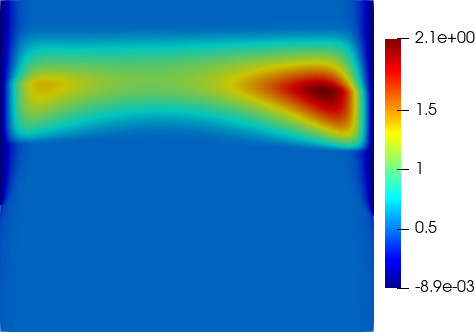
\includegraphics[width=\textwidth]{Figures/X.png}
    \caption{Phosphate ($X$)}
    \label{fig:baseparams_X}
\end{subfigure}
\qquad
\begin{subfigure}[t]{0.3\textwidth}
    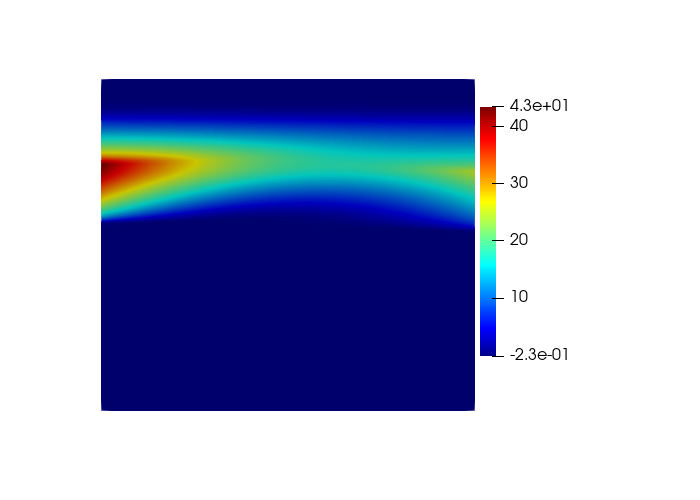
\includegraphics[width=\textwidth]{Figures/Y1.png}
    \caption{Phytase ($Y_1$)}
\end{subfigure}
\qquad
\begin{subfigure}[t]{0.3\textwidth}
    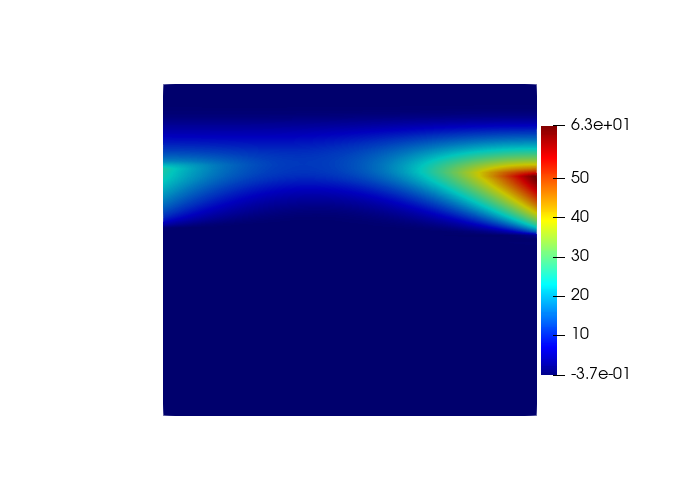
\includegraphics[width=\textwidth]{Figures/Y2.png}
    \caption{Citrate ($Y_2$)}
\end{subfigure}
\caption{Concentrations of the nutrients in the soil solution between the two roots after 24 hours.}
\label{fig:baseparams}
\end{figure}

%%%%%%%%%%%%%%%%%%%%%%%%%%%%%%%%%%%%%%%%%%%
\subsubsection{Citrate consumption by microbes}
\label{sec:numexp_vmax}
The first parameter change we experiment with is the assumption that citrate gets consumed by microbes in the soil, which we achieve by setting $V_{max} = 2.5 \times 10^{-9}$ mol kg$^{-1}$ s$^{-1}$ in the term for $Y_2$ decomposition $g_{Y,2} = \rho V_{max} Y_{L,2}/(K_M+Y_{L,2})$. Comparing the values in the colourbar of Fig. \ref{fig:numexp_vmax1} with Fig. \ref{fig:baseparams_X} we see that the maximum concentration of phosphate in the soil solution decreased by $\sim 30\%$. More important information on how much phosphate was actually absorbed by the root is shown in Fig. \ref{fig:numexp_vmax2} where we can see curves showing cumulative uptake in comparison with the benchmark result. The difference in phosphate uptake caused by citrate microbial consumption is shown in Table \ref{t:numexp_results}, reaching $-2.9\%$ and $-5.08\%$ in the left and right root, respectively. The amount of drop in phosphate absorption depends mainly on the uptake power of each of the roots (which are the same in this set-up) and on the citrate exudation rate of the corresponding root which is the reason why there was larger drop in the root on the right. The value of $V_{max}$ and the form of the citrate decompositon function was taken from the \ce{Zn-DMA} model in \cite{Ptashnyk-2011}, therefore the real dynamics for the actual decomposition of citrate may differ slightly.

\begin{figure}[!htb]
\centering
\begin{subfigure}[t]{0.45\textwidth}
    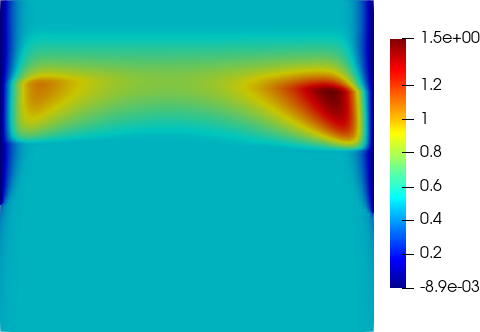
\includegraphics[trim= 100 100 60 100,width=\textwidth]{Figures/X_citrateVmaxnonzero.png}
    \caption{Phosphate ($X$)}
    \label{fig:numexp_vmax1}
\end{subfigure}
\qquad
\begin{subfigure}[t]{0.45\textwidth}
    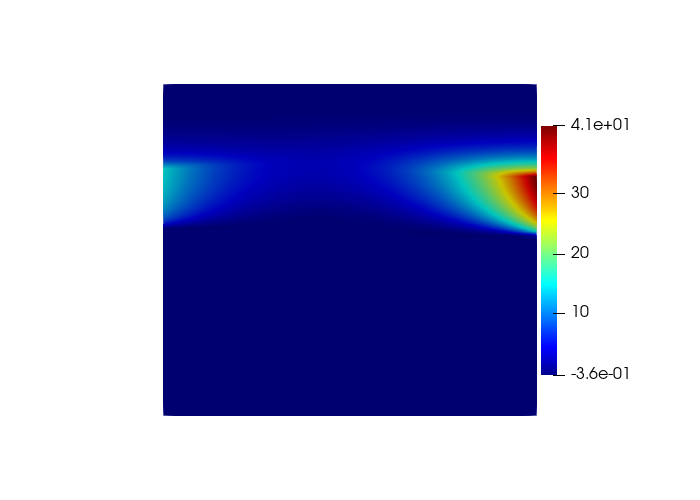
\includegraphics[trim= 100 100 60 100,width=\textwidth]{Figures/Y2_citrateVmaxnonzero.png}
    \caption{Citrate ($Y_2$).}
    \label{fig:numexp_vmax3}
\end{subfigure}
\qquad
\begin{subfigure}[t]{0.45\textwidth}
    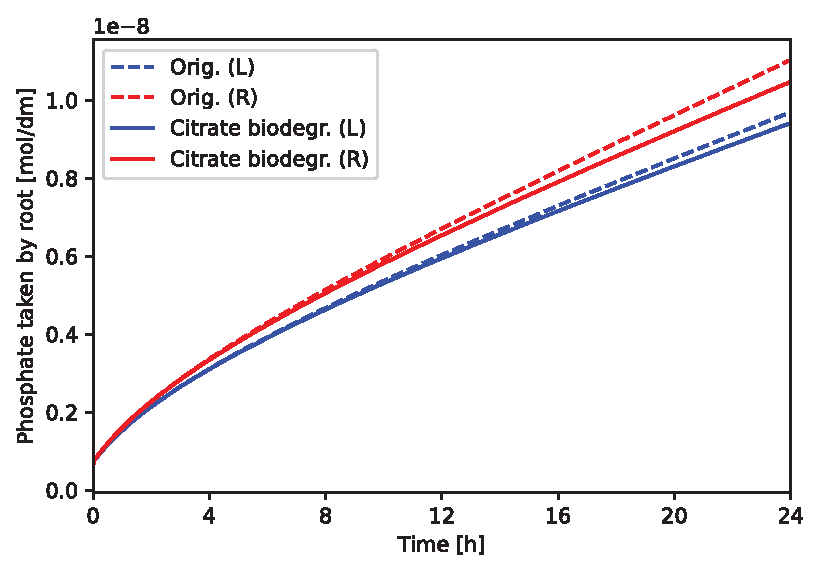
\includegraphics[width=\textwidth]{Figures/citratevmaxnonzero.eps}
    \caption{Cumulative uptake of phosphate by the left (L) and right (R) root.}
    \label{fig:numexp_vmax2}
\end{subfigure}
\caption{$V_{max} = 2.5 \times 10^{-9}$ mol kg$^{-1}$ s$^{-1}$, i.e. citrate gets consumed by microbes. In (a) concentration of phosphate and (b) citrate in soil solution between the two roots after 24 hours; (c) comparison of phosphate absorbed by each of the roots with original (dashed line) and changed parameters (solid line).}
\end{figure}

%%%%%%%%%%%%%%%%%%%%%%%%%%%%%%%%%%%%%%%%%%%
\subsubsection{Phosphate buffer power}
\label{sec:numexp_bx}
Next, we look at the buffer power $b_X$, which is defined as the ratio of absorption and desorption of phosphate to and from soil particles. First, we consider a twofold increase in $b_X$ which can be thought of as $b_X * 2 = \beta_1 / (0.5 \beta_2)$, i.e. we reduce the desorption rate by a half. The implications of this change can be observed in Fig. \ref{fig:numexp_bxup}. The results are somewhat counter-intuitive at first glance as we would expect that the decreased desorption rate (or equivalently, an increased absorption rate) would cause less phosphate to be absorbed by the root as it would stick to the soil particles instead of into the soil solution. We can also explain this algebraically by taking \eqref{x_2} and expressing the ratio between phosphate concentration in soil solution and soil solid,
\begin{equation}
    \frac{X_L}{X_S} = \frac{1}{b_X} + \kappa_{X,1} Y_{L,1} + \kappa_{X,2} Y_{L,2},
\end{equation}
we see that with increased $b_X$, the concentration of $X$ in soil solid increases at the expense of $X_L$. However, we can try to justify the results by supposing that the exudates operate on $P$ at soil particles, i.e. they solubilise $P$ they find at soil particles, and the more $P$ is found there (the higher the buffer power), the more of it gets solubilised into the solution and transported to the root surface. Citrate, in particular, pushes organic phosphate from the soil particles into the soil solution where phytase acts on it. This observation is very interesting as we didn't model the process into such details, and can be explored further in future work.

\begin{figure}[!htb]
\centering
\begin{subfigure}[t]{0.45\textwidth}
    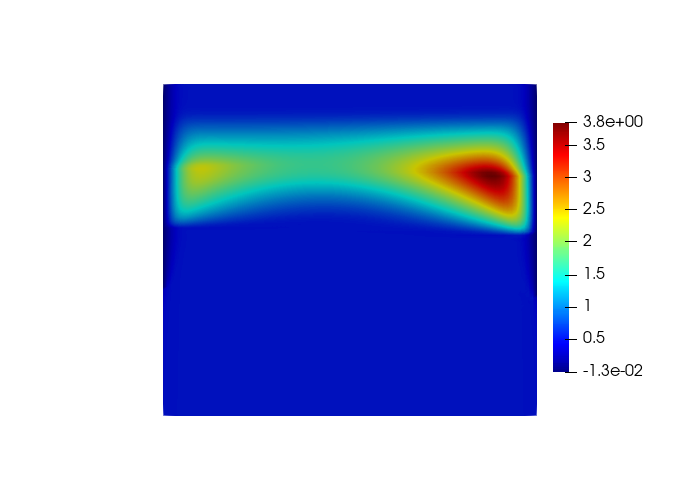
\includegraphics[trim= 100 100 60 100,width=\textwidth]{Figures/X_bXtimes2.png}
    \caption{Phosphate ($X$)}
    \label{fig:numexp_bxup1}
\end{subfigure}
\qquad
\begin{subfigure}[t]{0.45\textwidth}
    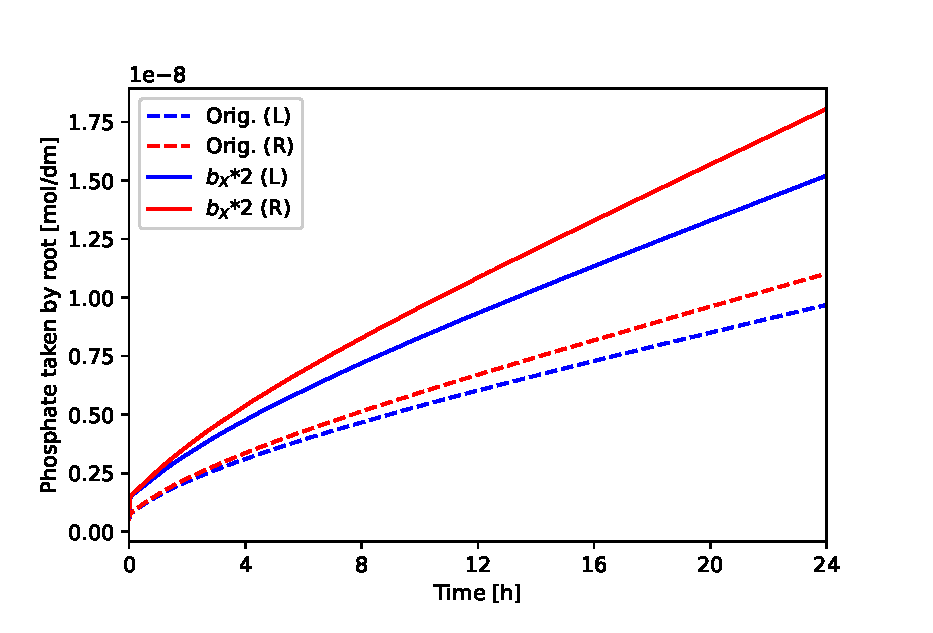
\includegraphics[width=\textwidth]{Figures/bxtimes2.eps}
    \caption{Cumulative uptake of phosphate by the left (L) and right (R) root.}
    \label{fig:numexp_bxup2}
\end{subfigure}
\caption{Buffer power $b_X$ multiplied by 2. In (a) concentration of phosphate between the two roots after 24 hours; (b) comparison of phosphate absorbed by each of the roots with original and changed parameters.}
\label{fig:numexp_bxup}

\end{figure}

We may consider the opposite of the previous scenario and divide $b_X$ by two, i.e. $b_X / 2 = \beta_1 / (2 \beta_2)$, so we increase the desorption rate from soil particles. We now know that this will have the opposite effect to what we have observed in Fig. \ref{fig:numexp_bxup}. In Fig. \ref{fig:numexp_bxdown2} we can see a decrease in phosphate uptake by both roots. Besides the huge difference between the range of values in Fig. \ref{fig:numexp_bxup1} and \ref{fig:numexp_bxdown1}, we notice in Table \ref{t:numexp_results} that decreased buffer power results in a greater absolute change in absorbed phosphate.

\begin{figure}[!htb]
\centering
\begin{subfigure}[t]{0.45\textwidth}
    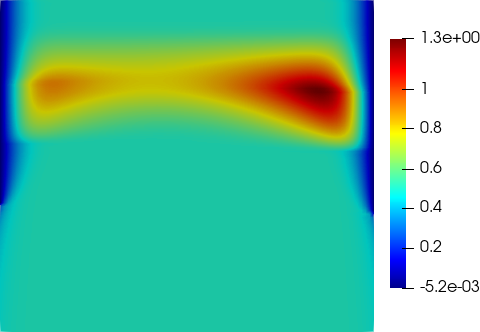
\includegraphics[trim= 100 100 60 100,width=\textwidth]{Figures/X_bXdivby2.png}
    \caption{Phosphate ($X$)}
    \label{fig:numexp_bxdown1}
\end{subfigure}
\qquad
\begin{subfigure}[t]{0.45\textwidth}
    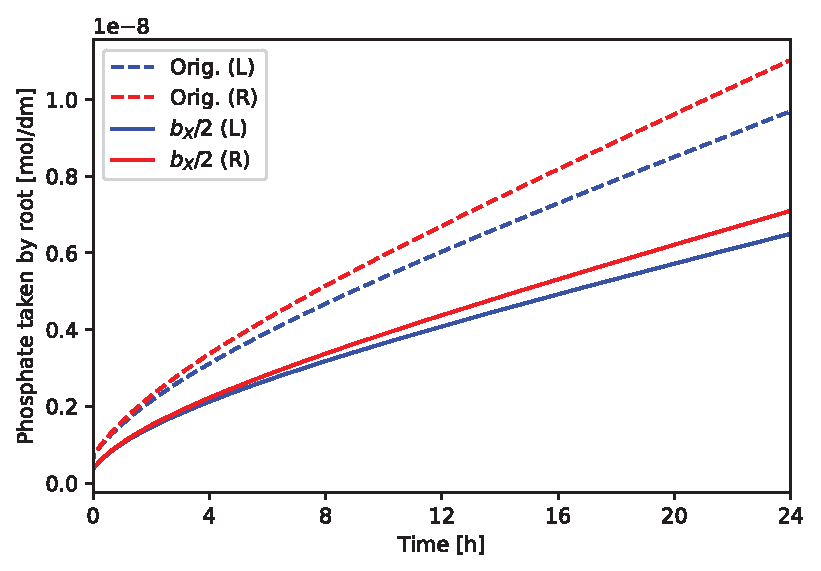
\includegraphics[width=\textwidth]{Figures/bxdivby2.eps}
    \caption{Cumulative uptake of phosphate by the left (L) and right (R) root.}
    \label{fig:numexp_bxdown2}
\end{subfigure}
\caption{Buffer power $b_X$ divided by 2. In (a) concentration of phosphate between the two roots after 24 hours; (b) comparison of phosphate absorbed by each of the roots with original and changed parameters.}
\label{fig:numexp_bxdown}
\end{figure}

%%%%%%%%%%%%%%%%%%%%%%%%%%%%%%%%%%%%%%%%%%%
\subsubsection{Uptake power at left root}
\label{sec:numexp_a1}
We now explore what effect does tenfold increase or decrease in uptake power of the left root, $\alpha_1$, have in comparison to the benchmark results. In Fig. \ref{fig:numexp_a1_up2} and \ref{fig:numexp_a1_down2} we see the expected increase and decrease in phosphate uptake by the left root. In Table \ref{t:numexp_results} we can observe that the tenfold raise in $\alpha_1$ caused $22.6 \%$ more phosphate to be absorbed, while tenfold drop in the uptake power resulted in decline by only $6 \%$. We can therefore assume that this root is more sensitive towards the increase in the uptake power. By comparing Fig. \ref{fig:numexp_a1_up1} and \ref{fig:numexp_a1_down1} we do not notice a major difference in $X_L$ besides a longer phosphate-deprived zone at the left edge of Fig. \ref{fig:numexp_a1_up1}.

\begin{figure}[!htb]
\centering
\begin{subfigure}[t]{0.45\textwidth}
    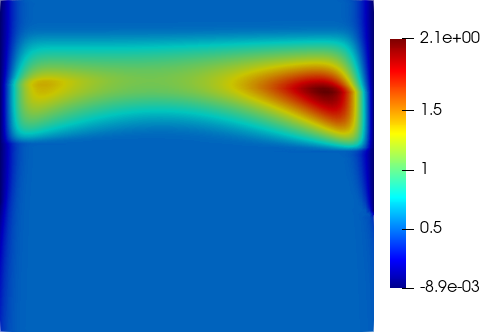
\includegraphics[trim= 100 100 60 100,width=\textwidth]{Figures/X_alpha1times10.png}
    \caption{Phosphate ($X$)}
    \label{fig:numexp_a1_up1}
\end{subfigure}
\qquad
\begin{subfigure}[t]{0.45\textwidth}
    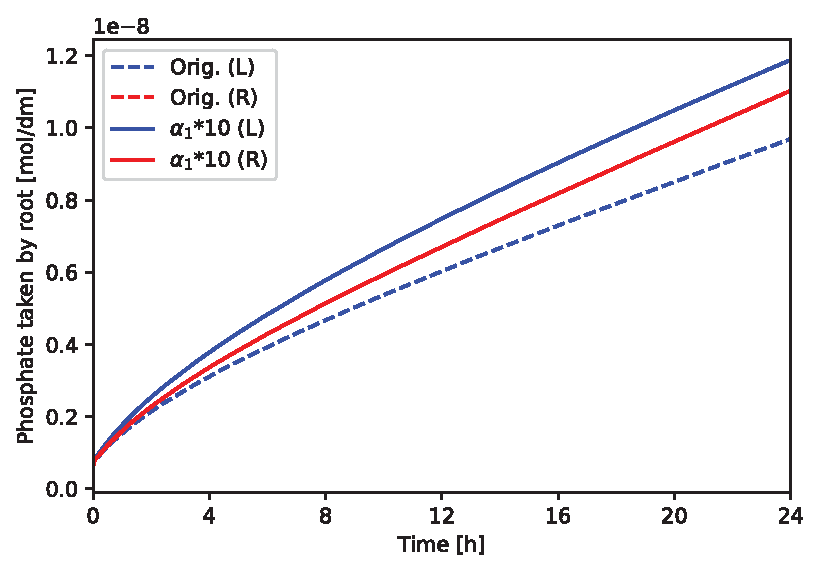
\includegraphics[width=\textwidth]{Figures/alpha1times10.eps}
    \caption{Cumulative uptake of phosphate by the left (L) and right (R) root.}
    \label{fig:numexp_a1_up2}
\end{subfigure}
\caption{Phosphate uptake power $\alpha_1$ multiplied by 10. In (a) concentration of phosphate between the two roots after 24 hours; (b) comparison of phosphate absorbed by each of the roots with original and changed parameters.}
\label{fig:numexp_a1_up}
\end{figure}

\begin{figure}[!htb]
\centering
\begin{subfigure}[t]{0.45\textwidth}
    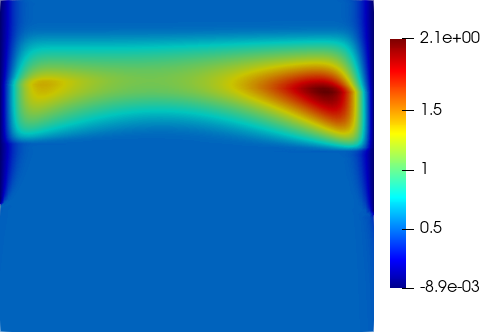
\includegraphics[trim= 100 100 60 100,width=\textwidth]{Figures/X_alpha1divby10.png}
    \caption{Phosphate ($X$)}
    \label{fig:numexp_a1_down1}
\end{subfigure}
\qquad
\begin{subfigure}[t]{0.45\textwidth}
    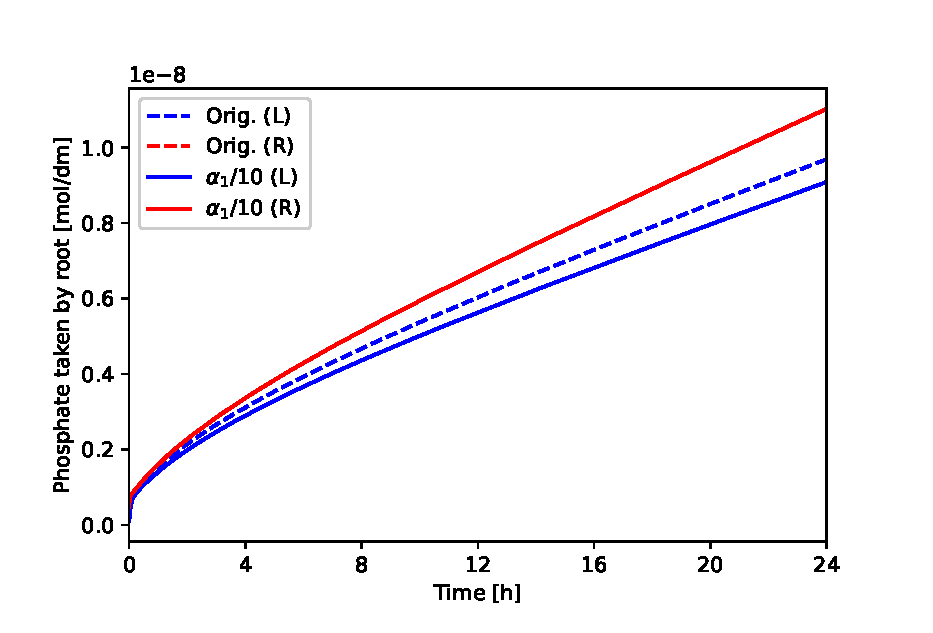
\includegraphics[width=\textwidth]{Figures/alpha1divby10.eps}
    \caption{Cumulative uptake of phosphate by the left (L) and right (R) root.}
    \label{fig:numexp_a1_down2}
\end{subfigure}

\caption{Phosphate uptake power $\alpha_1$ divided by 10. In (a) concentration of phosphate between the two roots after 24 hours; (b) comparison of phosphate absorbed by each of the roots with original and changed parameters.}
\label{fig:numexp_a1_down}
\end{figure}

%%%%%%%%%%%%%%%%%%%%%%%%%%%%%%%%%%%%%%%%%%%
\subsubsection{Diffusion coefficients}
We can experiment with the effect of an increase of diffusion coefficient on the transport of the chemicals in the rhisosphere. 


% \begin{figure}[!htb]
% \centering
% \begin{subfigure}[t]{0.45\textwidth}
%     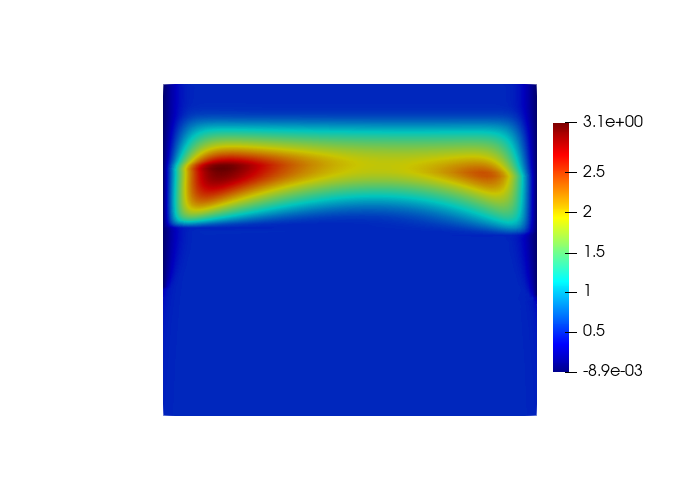
\includegraphics[trim= 100 100 60 100,width=\textwidth]{Figures/X_Fy11times10.png}
%     \caption{Phosphate ($X$)}
% \end{subfigure}
% \qquad
% \begin{subfigure}[t]{0.45\textwidth}
%     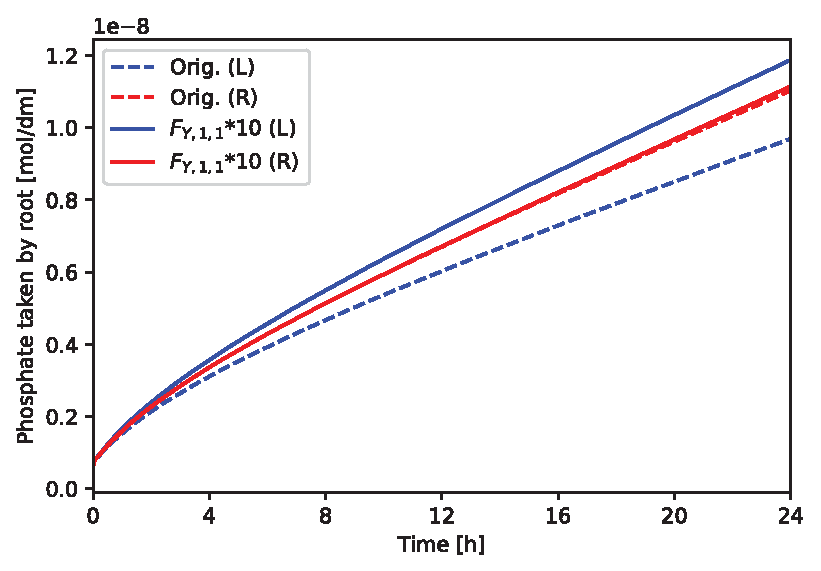
\includegraphics[width=\textwidth]{Figures/Fy11times10.eps}
%     \caption{Cumulative uptake of phosphate by the left (L) and right (R) root.}
% \end{subfigure}

% \caption{Phytase exudation rate power $F_{Y,1,1}$ multiplied by 10. In (a) concentration of phosphate between the two roots after 24 hours; (b) comparison of phosphate absorbed by each of the roots with original and changed parameters.}
% \end{figure}


%%%%%%%%%%%%%%%%%%%%%%%%%%%%%%%%%%%%%%%%%%%
\subsubsection{Phytase exudation rate at left root}
\label{sec:numexp_F11}



\begin{figure}[!htb]
\centering
\begin{subfigure}[t]{0.45\textwidth}
    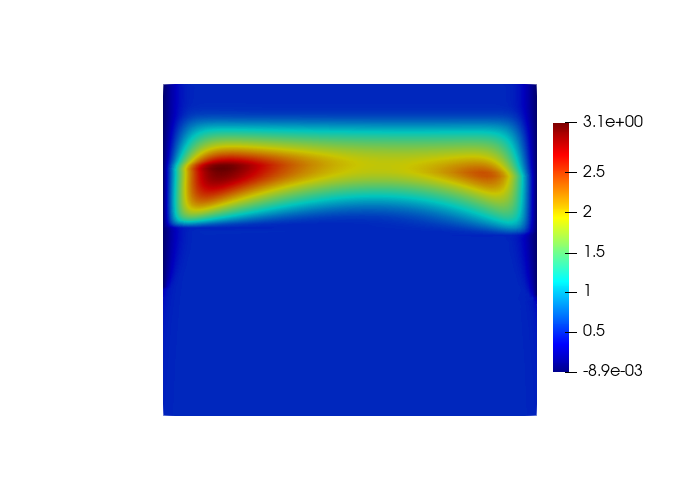
\includegraphics[trim= 100 100 60 100,width=\textwidth]{Figures/X_Fy11times10.png}
    \caption{Phosphate ($X$)}
\end{subfigure}
\qquad
\begin{subfigure}[t]{0.45\textwidth}
    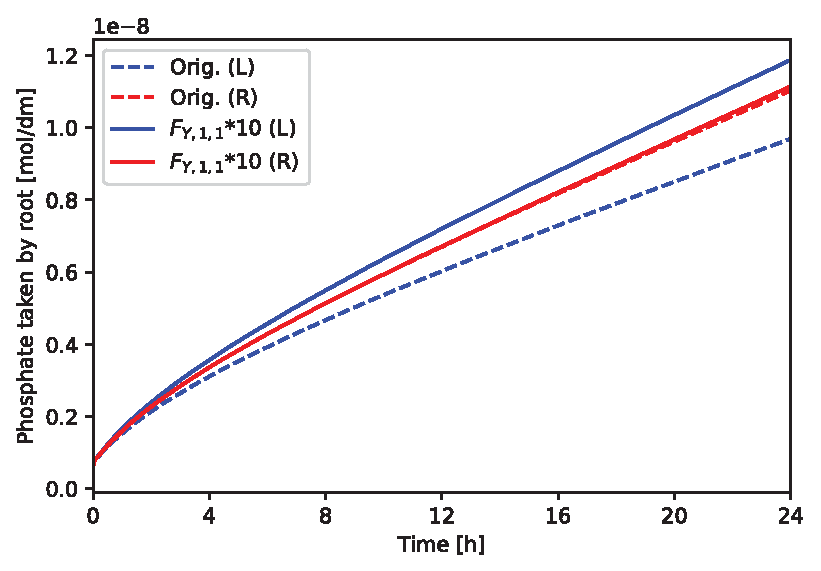
\includegraphics[width=\textwidth]{Figures/Fy11times10.eps}
    \caption{Cumulative uptake of phosphate by the left (L) and right (R) root.}
\end{subfigure}

\caption{Phytase exudation rate power $F_{Y,1,1}$ multiplied by 10. In (a) concentration of phosphate between the two roots after 24 hours; (b) comparison of phosphate absorbed by each of the roots with original and changed parameters.}
\end{figure}


\begin{figure}[!htb]
\centering
\begin{subfigure}[t]{0.45\textwidth}
    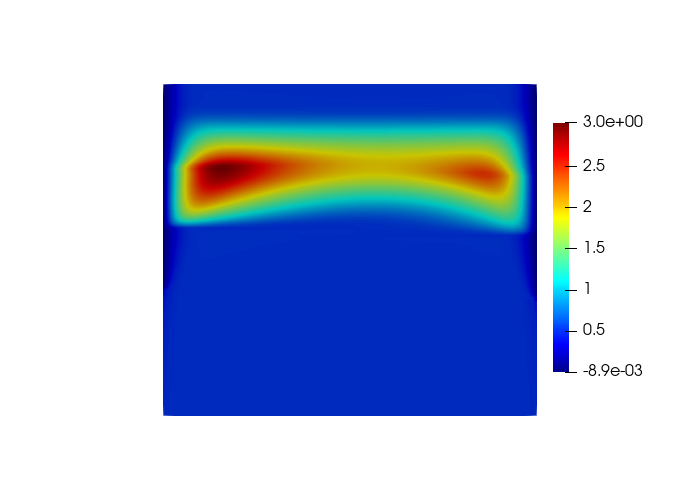
\includegraphics[trim= 100 100 60 100,width=\textwidth]{Figures/X_Fy11times10Y1up20pc.png}
    \caption{Phosphate ($X$)}
\end{subfigure}
\qquad
\begin{subfigure}[t]{0.45\textwidth}
    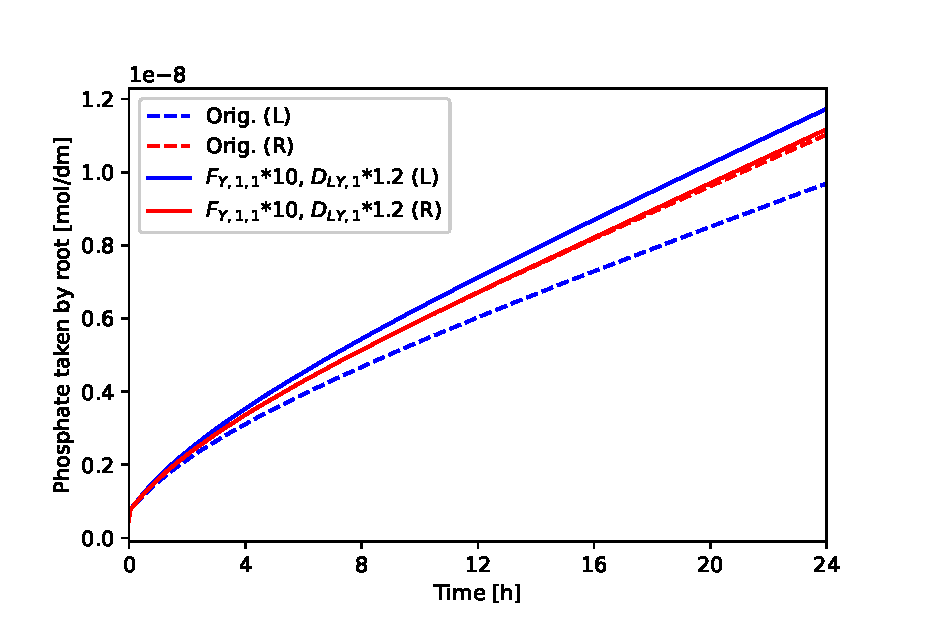
\includegraphics[width=\textwidth]{Figures/Fy11times10DY1up20pc.eps}
    \caption{Cumulative uptake of phosphate by the left (L) and right (R) root.}
\end{subfigure}

\caption{Phytase exudation rate power $F_{Y,1,1}$ multiplied by 10 combined with $20\%$ increase in diffusion of phytase $D_{LY,1}$. In (a) concentration of phosphate between the two roots after 24 hours; (b) comparison of phosphate absorbed by each of the roots with original and changed parameters.}
\end{figure}

\begin{table}[h]
\begin{center}

\fontsize{9.5}{7}\selectfont
\setlength{\tabcolsep}{5.pt}
\def\arraystretch{2.0}
\begin{tabular}{lrcccc}
\toprule
 & \multicolumn{2}{c}{\textbf{Total phosphate taken by root after 24h [mol dm$^{-1}$]}} & \multicolumn{2}{c}{\textbf{Change}} \\
 \hline
  \textbf{Section} & \textbf{Parameter change} & \textbf{Left root} & \textbf{Right root} & \textbf{Left root}  & \textbf{Right root}\\
 \hline 
Sec. \ref{sec:baseparams} & Base parameters & 9.689e$^{-9}$ &  1.103e$^{-8}$& - &- \\
Sec. \ref{sec:numexp_vmax}& Citrate $V_{max}=2.5 \times 10^{-9}$ & 9.409e$^{-9}$ & 1.047e$^{-8}$ & -2.9\% & -5.08\%\\
Sec. \ref{sec:numexp_bx} & Buffer power $b_x * 2$ & 1.521e$^{-8}$ & 1.806e$^{-8}$ & 57.0\% & 63.74\% \\
Sec. \ref{sec:numexp_bx} & Buffer power $b_x / 2$  & 6.495e$^{-9}$ & 7.095e$^{-9}$ & -33.0\% & -35.68\%\\
Sec. \ref{sec:numexp_a1} & Uptake power $\alpha_1 * 10$ & 1.188e$^{-8}$ & 1.103e$^{-8}$ & 22.6\% & 0.00\% \\
Sec. \ref{sec:numexp_a1} & Uptake power $\alpha_1 / 10$  & 9.087e$^{-9}$ & 1.103e$^{-8}$ & -6.2\% & 0.00\% \\
Sec. & $D_{LX}*1.2$ & 1.653e$^{-8}$ & 1.961e$^{-8}$ & 70.6\% & 77.79\% \\
Sec. & $D_{LY,1}*1.2$ & 1.516e$^{-8}$ & 1.805e$^{-8}$ & 56.5\% & 63.64\% \\
Sec. & $\{D_{LY,1}, D_{LY,2} \}*1.2$ & & \\
Sec. & $\{D_{LX}, D_{LY,1}, D_{LY,2} \}*1.2$ & & \\
Sec. & $F_{Y,1,1}*10$ & 1.187e$^{-8}$ & 1.114e$^{-8}$ & 22.5\% & 1.00\% \\
Sec. & $F_{Y,1,1}*10\text{ and } D_{Y1}*1.2$ & 1.173e$^{-8}$ & 1.117e$^{-8}$ & 21.1\% & 1.27\%   \\
\bottomrule
\end{tabular}
\caption{Total phosphate absorbed in each of the roots after 24 hours and change of resulting values with respect to results obtained by using the original (base) parameters defined in Table \ref{t:Second-model-params}. \label{t:numexp_results}}
\end{center}
\end{table}

\clearpage
\newpage
\subsection{Conclusions}
\textcolor{red}{How realistic the predictions are?}
\begin{itemize}
    \item assumptions and drawbacks of the model
    \item parameters are intertwined, the result depends on their combination
    \item interesting result with buffer power, can be changed by pH in the rhizosphere
    \item higher diffusion better, diffusion impacted by pH of the soil
    \item implications
    \item note that it's best for the plants to be in sync (with their growth rate and initial lengths, or with the exudation/absorption zones) for intercropping of this kind to be effective? 
    \item draw conclusions about the proximity of the roots from the experiments with the rice model
    \item future work
\end{itemize}
\newpage
\clearpage

%%%%%%%%%%%%%%%%%%%%%%%%%%%%%%%%%%%%%%%%%
%%%%%%%%%%%%%%%%%%%%%%%%%%%%%%%%%%%%%%%%%
%%%%%%%%%%%%%%%%%%%%%%%%%%%%%%%%%%%%%%%%%
\newpage
\section{Existence of Solutions}
\label{sec:Existence}

Taking into account the extensions of the original system from \cite{Ptashnyk-2011}, a more general version of system \eqref{eq:system-Zinc} is studied in this section. 

Let \(\Omega \subset \R^2\) be a rectangular domain, where we identify \(\Gamma := \partial \Omega\). Let \( Q := \Omega \times (0,T)\) for some fixed time \(T >0\).
Here, let \(y(x,t)\) and \(s(x,t)\) be vector functions from \(\Omega \times [0,T]\) in \(\R^{n}\) where for convenience we write \( x = (r,z) \in \Omega\) and also \(\Sigma = \Gamma \times (0,T)\). For each \(\ell \in \llb1,n\rrb\), let us define the uniformly elliptic operator \(L^\ell\) as
\[
	L^\ell y^\ell = \nabla \cdot (a^\ell \nabla y^\ell) + b^\ell \cdot \nabla y^\ell
	= \sum_{i=1}^{2}  \sum_{j=1}^2 \pd{ }{x_i} \big( a_{i,j}^\ell \pd{ }{x_j} y^\ell \big) + \sum_{i=1}^2 b_i^\ell \pd{ }{x_i} y^\ell,
\]
where \(a^\ell\), \(b^\ell \in L^\infty (Q)\), with \(a^\ell\) a matrix such that \(a^\ell_{i,i} \geq 0\) and
\(
	%\sum_{i=1}^{2}  \sum_{j=1}^2 a_{i,j}^\ell (x,t) \xi_i \xi_j \geq \theta |\xi|^2,
	\xi^\top (a^\ell (x,t) \xi) \geq \Theta |\xi|^2
\)
for some \(\Theta > 0\) and all \((x,t) \in Q\), \( \xi \in \R^2\).
%
Moreover, let \(F: \R^n \to \R^n\) such that each component \( F^\ell \) belongs to \( C^1 (\R) \cap L^\infty (\R)\), is Lipschitz continuous, and non negative for non negative arguments, and let \(h\in L^2 (\R^n,[0,T]) \) affine on \(y\), and such that \(h(0,t) \leq M \) for all \(t\).
Now, let \(G \in C^\infty(\R^{n+1}, \R^n)\) be bilinear such that each \( G^\ell(s,\cdot)\) is linear in \( y\) for fixed \(s\), and each \( G^\ell (\cdot, y)\) depends linearly only on \( s^\ell\) for fixed \(y\). Also, we assume that \(-G\) has the positiveness property that \(-G^\ell (0, y) \geq 0\) if \( y\geq 0\) component-wise. We will present a precise form for \(h\) and \(G\) later.
Finally, let the initial conditions be \( y_0, s_0^\ell \in L^\infty (\Omega)\) and non-negative.

We look after the solution of the system
\begin{subequations}
\label{eq:pde-ode-sys-a}
\begin{align}
	\pd{ }{t} y^\ell &= L^\ell y^\ell - y^\ell F^\ell(y^\ell) + G^\ell(s^\ell,y^1,\ldots y^n) 		&& \text{in } Q, \forall \ell \in \llb 1,n\rrb,
	\\
	\label{sys:coupled-ode}
	\pd{ }{t} s^\ell &= -G^\ell(s^\ell,y^1,\ldots y^n)				&& \text{in } Q,\forall \ell \in \llb 1,n\rrb,
	\\
	 (a^\ell \nabla y^\ell + y^\ell b^\ell) \cdot \vec{n} &= h^\ell (y^\ell, x,t)	&& \text{on } \Sigma,\forall \ell \in \llb 1,n\rrb,
	 \label{eq:1.2.d}
	 \\
	 y^\ell(0) &= y^\ell_{0}			 && \text{in } \Omega, \forall \ell \in \llb 1,n\rrb,
	 \\
	 s^\ell(0) &= s^\ell_{0}			 && \text{in } \Omega, \forall \ell \in \llb 1,n\rrb.
\end{align}
\end{subequations}
Here the set \( \llb 1,n\rrb\) is just the integer interval with extremes \(1\) and \(n\), namely
\[
	\llb 1,n\rrb = \{1,2,\ldots, n-1, n\}.
\]

We are interested in particular for \(G\) to be in the form
\begin{equation}
\label{eq:form_of_G}
	G^\ell (s^\ell,y) = \beta_0^\ell s^\ell - \gamma^\ell y^\ell + \sum_{\substack{1\le i\le n\\ i\neq \ell}} \beta_i^\ell y^i s^\ell,
\end{equation}
where for the positivity assumption we will require \( \gamma^\ell > 0\). We will further assume that \(\beta_i^\ell \geq 0\) for all \(i \in \llb 1,n\rrb \setminus\{\ell\}\) and \(\beta_0^\ell \geq 0\). Similarly, each component of \(h\) can be written as
\begin{equation}
\label{eq:form_of_h}
	h^\ell(y^\ell,x,t) = \alpha^\ell (x,t) y^\ell + \nu^\ell (x,t),
\end{equation}
with \(\nu^\ell \) a bounded function, and both \(\alpha^\ell \) and \(\nu^\ell \) integrable. Without loosing generality, let us assume further that \(\alpha^\ell \) and \(\nu^\ell \) are continuous and that \(\alpha^\ell \) is bounded as well. Finally, let us assume that \( \nu^\ell \geq 0\).


%%%%%%%%%%%%%%%%%%%%%%%%%%%%%%%%%%%%%%%%%%%%%%%%%%
%%%%%%%%%%%%%%%%%
\subsection{Analysis of the general coupled system}

In this section we will follow a similar procedure as \cite{Eisenhofer-2013,Ptashnyk-2010,Marciniak-2010}, and \cite{Ptashnyk-2016} to
determine and study a solution of coupled PDE-ODE systems. The scheme is as follows: (a) Show that for fixed \(y\) there is a unique solution of the ODE system. (b) Show that for fixed \(s\) and a linearisation on \(y\) there is a unique solution of the PDE system. (c) Show that the mapping that takes an initial \(y\) and solves the decoupled ODE-PDE system has a fixed point. 
Along this procedure the boundedness of solutions as well as their non negativity will be shown.

Let us begin defining the convex subspace of \((L^2 (Q))^n\):
\[
	Y = \big\{ y \in	(L^2 (Q))^n:\, 	%\big( 0,T, L^\infty(\Omega) \big): \, 
	0 \leq y(x,t) \leq \vartheta \quad\text{for a.e.}\quad (x,t) \in Q \big\}
\]
for a fixed \(\vartheta > 0\).
%
The existence of a solution of \eqref{eq:pde-ode-sys-a} is equivalent to the existence
of a fixed point of \(K\) defined on 
%\(L^2 \big( (0,T), (H^1(\Omega))^n \big) \cap Y \), 
\(Y\) %,
%
%
%\( L^2 (0,T,Z)\) with \(Z = \big( (H^1(\Omega))^n \times (L^2(\Omega))^n \big) \cap \big(L^\infty(\Omega)\big)^{2n}\) and its derivative in \(L^2 (0,T, Z^*) \). 
%\( L^2 (0,T,Y)\), with \(Y = \big(H^1(\Omega) \cap L^\infty(\Omega)\big)^{n}\) 
%
%
%and its derivative in \(L^2 ( 0,T;(H^1(\Omega))^{*n} )\),
by \( y_m = K(y_{m-1}) \), where \(y_m\) is a solution of the system
\begin{subequations}
\label{sys:de-coupled}
\begin{align}
	\pd{ }{t} y_m^\ell &= L^\ell y_m^\ell - y^\ell_m F^\ell(y_{m-1}^\ell) + G^\ell(s_m^\ell,y_{m}^1,\ldots y_{m}^n) 		&& \text{in } Q, \forall \ell \in \llb 1,n\rrb,
	\label{sys:de-coupled-pde}
	\\
	\pd{ }{t} s_m^\ell &= -G^\ell(s_m^\ell,y_{m-1}^1,\ldots y_{m-1}^n)				&& \text{in } Q,\forall \ell \in \llb 1,n\rrb,
	\label{sys:de-coupled-ode}
	\\
	 (a^\ell  \nabla y_m^\ell + y_m^\ell b^\ell) \cdot \vec{n} &= h^\ell (y_{m}^\ell, x,t)	&& \text{on } \Sigma,\forall \ell \in \llb 1,n\rrb,
	 \label{sys:de-coupled-pde-b}
	 \\
	 y_m^\ell(0) &= y^\ell_{0}			 && \text{in } \Omega, \forall \ell \in \llb 1,n\rrb,
	 \label{sys:de-coupled-pde-i}
	 \\
	 s_m^\ell(0) &= s^\ell_{0}			 && \text{in } \Omega, \forall \ell \in \llb 1,n\rrb.
	 \label{sys:de-coupled-ode-i}
\end{align}
\end{subequations}

Now we can divide the system in two parts. First, the analysis of the differential equations \eqref{sys:de-coupled-ode}, and then the analysis for the partial differential equations in \eqref{sys:de-coupled-pde}.

%%%%%%%%%%%%%%%
%%%%%%%%%%%%%%%
\vspace{1\baselineskip}
\noindent\emph{(A) Subsystem of ordinary differential equations}
\vspace{0.5\baselineskip}

Observe that for any given \(y_{m-1} \in Y \), then the ODE system \eqref{sys:de-coupled-ode}--\eqref{sys:de-coupled-ode-i} is a non-homogeneous linear system of ordinary differential equations.
%
Carathéodory's theorem gives us that there exists a unique solution \(s_m \in H^{1} ( 0,T;(L^2(\Omega))^{n}  )\) for some \(T\).
	%
	We can improve this regularity. Recalling \eqref{eq:form_of_G}, for any \(y_{m-1} \in Y\), \(-G(s_m,y_{m-1})\) can be written as
	\[
		-G(s_m,y_{m-1}) = B(y_{m-1})s_m + C(y_{m-1})
	\]
	with \(C\) a vector and \(B\) a diagonal matrix. As \(B(y)(t_1)\) commutes with \( B(y)(t_2)\), for any \(t_1, t_2 \in \R\) (as it is a diagonal matrix), we further have that there is a \(H^1 (0,T;(L^2(\Omega))^n )\) solution given by
	\[
		s_m(t) = e^{\overline{B}(t)} s_0 + \int\limits_0^t e^{\overline{B}(t)- \overline{B}(r)} C(y_{m-1}) \dif r
	\]
	with \( \overline{B}(t) = \int_0^t B(y_{m-1})(\xi) \dif \xi\) \cite{Schaeffer-2016}. 
	%
	Particularly, each row of \(s_m\) will be given exactly by
	\begin{equation}
	\label{eq:solution_of_ode}
		s_m^\ell (t) = s_0 \, e^{ \int_0^t B_{\ell,\ell} (y_{m-1})(\xi) \dif \xi } + \int\limits_0^t 
		e^{ \int_0^t B_{\ell,\ell} (y_{m-1})(\xi) \dif \xi - \int_0^r  B_{\ell,\ell} (y_{m-1})(\xi) \dif \xi} 
		C^{\ell} (y_{m-1})(r) \dif r.
	\end{equation}
	Here we have that
	\[
		B_{\ell,\ell} = -\beta_0^\ell - \sum_{\substack{1\le i\le n\\ i\neq \ell}} \beta_i^\ell y_{m-1}^i 
		\qquad\text{and}\qquad
		C^\ell (y_{m-1}) = \gamma^\ell y_{m-1}^\ell,
	\]
	where we have to recall that \( \gamma_i^\ell \geq 0\) and \( y_{m-1} \in Y\). As a result, \eqref{eq:solution_of_ode} yields an always non negative solution \( s_m \in L^\infty (Q)\).
	If we did not have a closed expression for \(s_m\), we could have argued via the work of \cite{Horvath-1998} on positiveness for ODE systems, which requires the positiveness assumption for \(-G\) and \(s_0\). In any case, we have got that \( s_m^\ell \in H^1(0,T;L^2(\Omega) ) \cap L^\infty (Q)\) and \(s_m^\ell \geq 0\) for each \(\ell\in \llb 1,n\rrb\) whenever \(y_{m-1} \in Y\).



%%%%%%%%%%%%%%%
%%%%%%%%%%%%%%%
\vspace{1\baselineskip}
\noindent\emph{(B) Subsystem of partial differential equations}
\vspace{0.5\baselineskip}


Next we turn to the linear system \eqref{sys:de-coupled-pde}, \eqref{sys:de-coupled-pde-b}, \eqref{sys:de-coupled-pde-i} of parabolic differential equations. Further, as we already have \(s_m\), it is now \emph{decoupled} from the ODE system. 
%Following \cite{Evans-2010}, we consider a different viewpoint by associating with \(u\) a mapping \( \mathbf{u} : [0,T] \to V\), such that \( \mathbf{u}(t)(x) = u(x,t)\), with \(V\) an appropriate Banach space. 

We say that a vector function \(y_m\) is a weak solution of \eqref{sys:de-coupled-pde} with boundary conditions \eqref{sys:de-coupled-pde-b} and initial conditions \eqref{sys:de-coupled-pde-i} if each \(y^\ell_m \in L^2(0,T;H^1(\Omega)) \) and \( \pd{y_m^\ell}{t} \in L^2(0,T;(H^1(\Omega))^*) \)  satisfy
\begin{equation}
\label{eq:linear-parabolic}
\begin{aligned}
	\int\limits_0^T %\int\limits_\Omega \pd{ y_m^\ell}{t} v  \dif x 
	    \big\langle \pd{ y_m^\ell}{t}, v \big\rangle
	\dif t
	&=
	-
	\int\limits_0^T 
	\int\limits_\Omega (a^\ell \nabla y_m^\ell + y_m^\ell b^\ell ) \cdot \nabla v \dif x \dif t
	+
	\int\limits_0^T 
	\int\limits_\Gamma h^\ell (y_{m}^\ell,x,t) v \dif \sigma\dif t 
	\\ &\qquad\qquad\qquad
	+
	\int\limits_0^T \int\limits_\Omega 
	-y_m^\ell F^\ell(y^\ell_{m-1}) v + G^\ell(s_m^\ell, y_{m-1}) v \dif x \dif t
\end{aligned}
\end{equation}
for all \( v \in L^2 (0,T;H^1(\Omega) ) \), and with the initial condition \( y_m^\ell \to y_0^\ell \) in \(L^2(\Omega)\) as \( t\to 0\), for all \(\ell \in \llb 1,n\rrb\). 
Here we have used the duality pairing \(\langle \cdot, \cdot \rangle\) of \( (H^1(\Omega))^*\) and \( H^1(\Omega)\).
	
Problem \eqref{eq:linear-parabolic} has been extensively studied in the literature, see for example \cite{Ladyzenskaja-1968} or \cite{Pao-1993}. Using Galerkin's method, we can prove that there is a unique solution given component-wise as the element \(y_m^\ell \in L^2(0,T;\)  \( H^1(\Omega)) \cap L^\infty(0,T; L^2(\Omega))\) with \( \pd{y_m^\ell}{t} \in L^2(0,T; (H^1(\Omega))^*) \).



%%%%%%%%%%%%%%%
%%%%%%%%%%%%%%%
%%%%%%%%%%%%%%%
%\subsubsection{Proof of existence of \(y_m\)}
\vspace{1\baselineskip}
\noindent\textbf{Proof of existence of \(y_m\)}
\vspace{0.5\baselineskip}
	
	We will adapt ideas from \cite{Ladyzenskaja-1968,Troltzsch-2010} and \cite{Evans-2010}.
	
	Consider a fundamental system of functions \((w_k)_{k\in \N^*}\) in \(H^1(\Omega)\); i.e., they form an orthogonal basis in \(H^1(\Omega)\), and for simplicity let us assume further that they are orthonormalised in \(L^2(\Omega)\). Moreover, let us define\footnote{Notice that \(a^\ell\) is linear in \( y_m\), not only in \(y_m^\ell\).}
	\[
		a^\ell [ y_m,v;t] := 
		\int\limits_\Omega (a^\ell \nabla y_m^\ell + y_m^\ell b^\ell ) \cdot \nabla v \dif x + \int\limits_\Omega d^\ell (y_m) v \dif x
		- \int\limits_\Gamma \alpha^\ell (x,t) y_m^\ell v \dif \sigma
	\]
	where we have used the explicit form of \(h^\ell\) presented in \eqref{eq:form_of_h}, and \(d^\ell\) is given by
	\[
		d^\ell (y_m) := y_m^\ell F^\ell(y_{m-1}^\ell) + \gamma^\ell y_m^\ell - s_m^\ell \sum_{\substack{1\le i\le n\\ i\neq \ell}} \beta_i^\ell y_m^i.
	\]
	Also let us define the two linear functionals in \(v\)
	\[
		\mathbf{f}^\ell (t) := \beta_0^\ell \int\limits_\Omega s_m^\ell  v \dif x
		\qquad\text{and}\qquad
		\mathbf{g}^\ell (t) :=  \int\limits_\Gamma \nu^\ell (x,t)  v \dif \sigma.
	\]
	Notice that these are well defined as \(F^\ell\) and \(s_m^\ell\) are bounded.
	
	
	
	
	
	Fix a positive integer \(N\). We will seek for an approximate solution in the form
	\begin{equation}
	\label{eq:ansatz}
		\mathbf{y}_m^{\ell,N} (t)(x) = \sum_{k=1}^N c_k^{\ell,N} (t) w_k(x)
	\end{equation}
	so that the coefficients \( c_k^{\ell,N} \) are determined by
	\begin{equation}
	\label{sys-pde-pre-galerkin}
		\big(\pd{ }{t}  y_m^{\ell,N}, w_k\big)_\Omega + 
		a^\ell [y_m^{N}, w_k; t] 
		=
		\big( \mathbf{f}^\ell (t), w_k \big)_{\Omega} + \big(\mathbf{g}^\ell (t),  w_k \big)_{\Gamma}
	\end{equation}
	for almost every \(t\in (0,T)\) with the initial condition \( c_k^N (0) =  ( y^\ell (0), w_k)_\Omega = (y_0^\ell, w_k)_\Omega\)  for all \(k \in \llb 1,N\rrb\); where
	%
	%Substituting the \emph{ansatz}  \eqref{eq:ansatz} in \eqref{sys-pde-pre-galerkin} and making use of the orthonormality, we see that
	\begin{align*}
		a^\ell [y_m^{N}, w_k; t] 
		&= 
		\sum_{i=1}^N  \bigg[ c_i^{\ell,N}  \int\limits_\Omega  ( a^\ell \nabla w_i + w_i b^\ell) \cdot \nabla w_k \dif x -  c_i^{\ell, N} \int\limits_\Gamma \alpha^\ell w_i w_k \dif \sigma
		\\
		&\qquad
		+ \int\limits_\Omega 
		c_i^{\ell,N} (w_i F^\ell w_k) + \frac{1}{N}  \gamma^\ell c_k^{\ell,N} -  \sum_{\substack{1\le j\le n\\ j\neq \ell}} \beta_j^\ell c_i^{j,N} (s_{m}^\ell w_i w_k)
		 \dif x
		\bigg] =: A^\ell (c^{N})
	\end{align*}
	Using orthogonality and orthonormality of \((w_k)_{k\in \N^*}\), we obtain the system
	\begin{subequations}
	\label{sys-pde-galerkin}
	\begin{align}
		\od{ }{t} c_k^{\ell,N} + A^\ell (c^{N}) &= l_k^\ell (t)		\\
		c_k^{\ell,N} (0) &= (y_0^\ell, w_k)
	\end{align}
	\end{subequations}
	for almost every \(t\in (0,T)\), all \( k\in \llb1,N\rrb\), and \(n\in \llb 1,n\rrb\); with the functions \( l^\ell_k(t) = \big( \mathbf{f}^\ell (t), w_k \big)_{\Omega} + \big(\mathbf{g}^\ell (t),  w_k \big)_{\Gamma}\).
	
	The system \eqref{sys-pde-galerkin} is a system of linear ordinary differential equations in terms of \(c_k^{\ell,N}\) with initial value conditions. Owing to Carathèodory's theorem, there exists a unique solution \( c^N \in \big(H^1(0,T)\big)^{nN}\). Now, if we put \(c^{\ell,N}\) as a test function in \eqref{sys-pde-pre-galerkin} and sum over \(k\), we get that
	\begin{equation}
	\label{eq:result-galerkin}
		\big(\pd{ }{t}  y_m^{\ell,N},  y_m^{\ell,N}\big)_\Omega + 
		a^\ell [ y_m^{N},  y_m^{\ell,N}; t] 
		=
		\big( \mathbf{f}^\ell (t),  y_m^{\ell,N} \big)_{\Omega} + \big(\mathbf{g}^\ell (t),   y_m^{\ell,N} \big)_{\Gamma}
	\end{equation}
	for almost every \(t\in (0,T)\) and all \(\ell \in \llb 1,n\rrb\). 
	
	 Now, for an arbitrary but fixed \(\tau \in (0,T]\) and any \(\ell \in \llb 1,n\rrb\), we have the identity 
	 \[
	 	\int\limits_0^\tau \big(\pd{ }{t}  y_m^{\ell,N}(t),  y_m^{\ell,N} (t) \big)_\Omega \dif t
		=
		\frac{1}{2} \int\limits_0^\tau  \pd{ }{t} \|  y_m^{\ell,N}(t) \|_\Omega^2 \dif t
		=
		\frac{1}{2} \|  y_m^{\ell,N}(\tau) \|_\Omega^2 - \frac{1}{2} \|  y_m^{\ell,N}(0) \|_\Omega^2.
	 \]
	 If we integrate \eqref{eq:result-galerkin} over \([0,\tau]\) and incorporate this last identity, we get that for any \(\ell \in \llb 1,n\rrb\) it holds
	 \begin{align}
	 \label{eq:estimate-integrationbyparts}
	 	\frac{1}{2} \|  y_m^{\ell,N}(\tau) \|_\Omega^2
		+ 
		\int\limits_0^\tau a^\ell [ y_m^{N},  y_m^{\ell,N}; t] \dif t
		=
		\frac{1}{2} \|  y_m^{\ell,N}(0) \|_\Omega^2 + 
		\int\limits_0^\tau \big( \mathbf{f}(t),  y_m^{\ell,N} (t) \big)_{\Omega} + \big(\mathbf{g}(t),   y_m^{\ell,N} (t) \big)_\Gamma \dif t.
	 \end{align}
	Additionally, by Bessel's inequality, we have that
	\begin{equation}
	\label{eq:estimate-i}
		\|  y_m^{\ell,N}(0) \|_\Omega^2 = \sum_{k=1}^N |c_k^{\ell,N}(0)|^2 = \sum_{k=1}^N | (y_0^\ell, w_k) |^2 \leq \|y_0^\ell\|_\Omega^2.
	\end{equation}
	
	
	
	Moreover, it is not hard to show, using Cauchy's inequality, that for any element \(v\in (H^1(\Omega))^n\) the inequality
	\[
		\frac{1}{2} {\Theta} \|\nabla v^\ell \|^2_{\Omega}
		\leq a^\ell [v,v^\ell;t]  + \frac{1}{2} C_{s,b,\alpha,F}^\ell \sum_{k=1}^n \|v^k\|^2_{\Omega} 
	\]
	is satisfied, where \(C_{s,b,\alpha,F}^\ell\) is a constant depending linearly on the supremum norms of \(s_m^\ell, b^\ell, \alpha^\ell\), and \(F^\ell(y_{m-1}^\ell)\). Furthermore, applying Cauchy's inequality again we get
	\[
		\big| \big( \mathbf{f}^\ell ,  y_m^{\ell,N} \big)_{\Omega} \big| \leq \frac{1}{2} \|\mathbf{f}^\ell \|^2_{\Omega} + \frac{1}{2} \| y_m^{\ell,N}\|_{\Omega}^2
		\qquad\text{and}\qquad
		\big(\mathbf{g}^\ell ,   y_m^{\ell,N} \big)_\Gamma
		\leq \varepsilon \|\mathbf{g}^\ell \|^2_{\Gamma} + \frac{1}{4\varepsilon} \| y_m^{\ell,N}\|_{\Gamma}^2.
	\]
	This way we can use a proper selection of \(\varepsilon\) alongside the trace inequality \cite{Evans-2010} to obtain, for some \(C_1\) and \(C_2\), that
	\[
		\od{ }{t} \|  y_m^{\ell,N} \|^2_\Omega + {\Theta} \|\nabla  y_m^{\ell,N}\|^2_{\Omega}
		\leq C_1 \sum_{k=1}^n \| y_m^{k,N}\|^2_{\Omega} + C_2\big(\|\mathbf{f}^\ell \|^2_{\Omega} + \|\mathbf{g}^\ell \|^2_{\Gamma} \big).
	\]
	\begin{comment}
	Adding the norm of \( y_m^{\ell,N}\) at both sides of the inequality, we get
	\[
		\od{ }{t} \|  y_m^{\ell,N} \|^2_\Omega + {\Theta} \|  y_m^{\ell,N}\|^2_{H^1(\Omega)}
		\leq C_1 \sum_{k=1}^n \| y_m^{k,N}\|^2_{H^1(\Omega)} + C_2\big(\|\mathbf{f}^\ell\|^2_{\Omega} + \|\mathbf{g}^\ell\|^2_{\Gamma} \big),
	\]
	with an updated \(C_1\). 
	\end{comment}
	We can sum the inequalities with respect to \(\ell\) to obtain
	\begin{equation}
	\label{eq:estimate-differential}
		\od{ }{t} \sum_{\ell=1}^n \|  y_m^{\ell,N} \|^2_\Omega + {\Theta} \sum_{\ell=1}^n \| \nabla  y_m^{\ell,N}\|^2_{\Omega}
		\leq C_1 \sum_{\ell=1}^n \| y_m^{\ell,N}\|^2_{\Omega} + C_2 \sum_{\ell=1}^n \big(\|\mathbf{f}^\ell\|^2_{\Omega} + \|\mathbf{g}^\ell\|^2_{\Gamma} \big),
	\end{equation}
	with updated \(C_1\) and \(C_2\).
	%
	Notice that this is a differential inequality, so we can use Grönwall's inequality \cite{Evans-2010} to get the estimate
	\begin{equation}
	\label{eq:Grownwall}
		\sum_{\ell=1}^n \|  y_m^{\ell,N} (t) \|^2_\Omega \leq \sum_{\ell=1}^n  e^{C_1 t} \bigg(  \|  y_m^{\ell,N} (0) \|^2_\Omega
			+ C_2 \int\limits_0^t \|\mathbf{f}^\ell (r)\|^2_{\Omega} + \|\mathbf{g}^\ell (r)\|^2_{\Gamma} \dif r
		\bigg).
	\end{equation}
	Now, by \eqref{eq:estimate-i} and the fact that \eqref{eq:Grownwall} is a sum of positive terms, we get the particular estimate
	\begin{equation}
	\label{eq:estimate-maxnorm}
		\max_{0\leq t \leq T} \|  y_m^{\ell,N} (t) \|^2_\Omega \leq C \sum_{k=1}^n  \bigg(  \|  y_0^k \|^2_\Omega
			+ \|\mathbf{f}^k\|^2_{L^2(0,T;L^2(\Omega))} + \|\mathbf{g}^k\|^2_{L^2(0,T;L^2(\Gamma))}
		\bigg)
	\end{equation}
	for each \(\ell \in \llb 1,n\rrb\).
	
	Now we can use \eqref{eq:estimate-integrationbyparts} replacing \(\tau\) with \(T\), estimate \eqref{eq:estimate-differential} completing the \(H^1\)--norm of each \(y_m^{\ell,N}\), and estimate \eqref{eq:estimate-maxnorm} to get
	\[
		\| y_m^{\ell,N} \|^2_{L^2(0,T, H^1(\Omega))}
		\leq 
		C \sum_{k=1}^n \bigg(  \|  y_0^k \|^2_\Omega + \|\mathbf{f}^k\|^2_{L^2(0,T, L^2(\Omega))} + \|\mathbf{g}^k\|^2_{L^2(0,T, L^2(\Gamma))} \bigg),
	\]
	where \(C\) is a generic positive constant. With these estimates we have got that
	\[
		\|  y_m^{\ell,N} \|^2_{L^\infty (0,T;L^2(\Omega) )} 
		+ \| y_m^{\ell,N} \|^2_{L^2(0,T;H^1(\Omega))}
		\leq 
		C \sum_{k=1}^n \bigg(  \|  y_0^k \|^2_\Omega + \|\mathbf{f}^k\|^2_{L^2(0,T;L^2(\Omega))} + \|\mathbf{g}^k\|^2_{L^2(0,T;L^2(\Gamma))} \bigg);
	\]
	%or alternatively, that the \(V_2(Q)\) norm of \( y_m^{\ell,N}\) is bounded by a constant independent of \(N\) and \(\ell\), let us call it \(K_{m}\). 
	where the term on the right-hand side is a constant independent of \(N\), let us call it \(K_{m}\). 
	Observe that in particular \eqref{eq:estimate-maxnorm} yields \( \| y_m^{\ell,N}(t)\|_{\Omega}^2 \leq K_{m} \)  for all \(t\in [0,T]\), and in view of the orthonormality
	\begin{equation}
	\label{eq:boundness-of-coeffs}
		\sum_{k=1}^N |c_k^N(t)|^2 \leq K_{m}
	\end{equation}
	for all \(t\in [0,T]\) and \( N \in \N^*\).
	
	We can even go a step further. Fix any \(v\in H^1(\Omega)\) with \(\|v\|_{H^1(\Omega)} \leq 1\) and write it as \( v = v^1 + v^2\), where \(v^1\) is generated by the span of \( \{w_k\}_{k=1}^N\) and \( (v^2,w_k) = 0\) for all \( k \in \{1,\ldots,N\}\). Since the functions \( (w_k)_{k\in \N^*}\) are orthogonal in \(H^1(\Omega)\), we get \( \|v^1\|_{H^1(\Omega)} \leq \|v\|_{H^1(\Omega)} \leq 1 \). Utilising \eqref{sys-pde-pre-galerkin}, we get that for almost every \(t\in (0,T)\)
	\[
		\big(\pd{ }{t}  y_m^{\ell,N}, v^1\big)_\Omega + 
		a^\ell [ y_m^{N}, v^1; t] 
		=
		\big( \mathbf{f}^\ell (t), v^1 \big)_{\Omega} + \big(\mathbf{g}^\ell (t),  v^1 \big)_{\Gamma}.
	\]
	Then \eqref{eq:ansatz} implies
	\[
		\big\langle \pd{ }{t}  y_m^{\ell,N}, v \big\rangle =
		\big(\pd{ }{t}  y_m^{\ell,N}, v\big)_\Omega =
		\big(\pd{ }{t}  y_m^{\ell,N}, v^1\big)_\Omega 
		=
		\big( \mathbf{f}^\ell (t), v^1 \big)_{\Omega} + \big(\mathbf{g}^\ell (t),  v^1 \big)_{\Gamma}
		- a^\ell [y_m^{N}, v^1; t] .
	\]
	Continuity of \(a^\ell\) and the norm of \(v\) with by Cauchy--Bunyakovsky--Schwarz inequality give
	\[
		\Big| \big\langle \pd{ }{t}  y_m^{\ell,N}, v \big\rangle \Big|
		\leq C \sum_{k=1}^n
		\big( \|\mathbf{f}^k\|_{\Omega} + \|\mathbf{g}^k\|_{\Gamma} + \| y_m^{k,N}\|_{H^1(\Omega)} \big);
	\]
	thus the operator norm of \(\pd{ }{t}  y_m^{\ell,N}\) is bounded for almost everywhere \(t\in (0,T)\). Additionally, we can square the last inequality, use again Cauchy's inequality and get
	\[
		\big\| \pd{ }{t}  y_m^{\ell,N} \big\|_{(H^1(\Omega))^*} 
		\leq C \sum_{k=1}^n \big( \|\mathbf{f}^k\|_{\Omega} + \|\mathbf{g}^k\|_{\Gamma} + \| y_m^{k,N}\|_{H^1(\Omega)} \big) ;
	\]
	and therefore
	\begin{align*}
		\int\limits_0^T \big\| \pd{ }{t}  y_m^{\ell,N} \big\|^2_{(H^1(\Omega))^*} \dif t 
		\leq C\sum_{k=1}^n \bigg(  \|  y_0^k \|^2_\Omega + \|\mathbf{f}^k\|^2_{L^2(0,T, L^2(\Omega))} + \|\mathbf{g}^k\|^2_{L^2(0,T, L^2(\Gamma))} \bigg).
	\end{align*}
	As a result, we have got
	\begin{equation}
	\label{eq:energy-estimates}
	\begin{aligned}
		\|  y_m^{\ell,N} \|^2_{C([0,T];L^2(\Omega) )} 
		&+ \| y_m^{\ell,N} \|^2_{L^2(0,T; H^1(\Omega))}
		+  \| \partial_t  y_m^{\ell,N} \|^2_{L^2(0,T;H^1(\Omega)^*)}
		\\
		&\qquad\qquad\leq 
		C \sum_{k=1}^n \bigg(  \|  y_0^k \|^2_\Omega + \|\mathbf{f}^k\|^2_{L^2(0,T;L^2(\Omega))} + \|\mathbf{g}^k\|^2_{L^2(0,T;L^2(\Gamma))} \bigg).
	\end{aligned}
	\end{equation}
	
	%
	% Made it!
	%
	According to the energy estimates \eqref{eq:energy-estimates} and \eqref{eq:boundness-of-coeffs}, we see that \(( y_m^{\ell,N})_{N\in \N^*}\) is bounded in \(L^2(0,T;H^1(\Omega))\), \((\partial_t  y_m^{\ell,N})_{N\in \N^*}\) is bounded in \(L^2(0,T;H^1(\Omega)^*)\), and all \( c_k^{\ell,N} (t)\) are essentially bounded for all \(\ell\), \(k\), \(N\), and \(t\). 
	Consequently, there exists a subsequence \(( y_m^{\ell,N_q})_{N_q\in \N}\) and functions \( y_m^{\ell} \in L^2(0,T;H^1(\Omega))\),  with \(\pd{ }{t} y_m^{\ell} \in L^2(0,T;(H^1(\Omega))^*)\) for each \(\ell \in \llb1,n\rrb\), such that
	\begin{equation}
	\label{weak-conv}
		\begin{cases}
			 y_m^{\ell,N_q} \rightharpoonup  y_m^{\ell} & \text{weakly in } L^2(0,T;H^1(\Omega)),
			\\
			\pd{ }{t} y_m^{\ell,N_q} \rightharpoonup \pd{ }{t}  y_m^{\ell} & \text{weakly in } L^2(0,T;H^1(\Omega)^*).
		\end{cases}
	\end{equation}
	Moreover, owing to the weak lower sequential semicontinuity of the norm, we also get that \(\| y_m^\ell(t)\|_\Omega\) is also bounded by \(K_{m}\) for all \(t\in [0,T]\), thus \( y_m^\ell \in L^\infty (0,T; L^2 (\Omega))\).



Now, for a fixed integer \(\tilde n\), let us pick a function \( \bv \in C^1([0,T]; H^1(\Omega))\) of the form
	\begin{equation}
	\label{eq:test-fun-bochner}
		\bv(t) = \sum_{k=1}^{\tilde n} d_k(t) w_k,
	\end{equation}
	with \(\{d_k\}_{k=1}^{\tilde n}\) a set of given functions.
	Let us pick \(N \geq \tilde n\), multiply \eqref{sys-pde-pre-galerkin} by \(c_k\), sum over \(k\) and then integrate with respect to \(t\) to find
	\[
		\int\limits_0^T
		\big\langle \pd{ }{t}  y_m^{\ell,N}, \bv \big\rangle + 
		a^\ell [y_m^{N}, \bv; t] \dif t
		=
		\int\limits_0^T
		\big( \mathbf{f}^\ell (t), \bv \big)_{\Omega} + \big(\mathbf{g}^\ell (t),  \bv \big)_{\Gamma}
		\dif t.
	\]
	Using the subsequence and recalling \eqref{weak-conv} and taking limit \(N\to \infty\), we get
	\begin{equation}
	\label{eq:variational}
		\int\limits_0^T
		\big\langle \pd{ }{t}  y_m^{\ell}, \bv \big\rangle + 
		a^\ell [y_m^{\ell}, \bv; t] \dif t
		=
		\int\limits_0^T
		\big( \mathbf{f}^\ell (t), \bv \big)_{\Omega} + \big(\mathbf{g}^\ell (t),  \bv \big)_{\Gamma}
		\dif t.
	\end{equation}
	This equality then holds for all functions \( \bv \in L^2(0,T;H^1(\Omega))\), as functions of the form \eqref{eq:test-fun-bochner} are dense in this space. %In particular, it holds for any \( v \in H^1(\Omega)\) as well. 
	
	To prove that \(  y_m^\ell (0) = y_0^\ell\) it suffices to see that \eqref{eq:result-galerkin} can be integrated by parts in time for all \( \bv \in C^1(0,T;H^1(\Omega))\) with \(\bv(T) = 0\) \cite{Evans-2010}. Again passing through a subsequence, noticing that \(  y_m^{\ell, N_k} (0) \to y_0^\ell\) in \(L^2(\Omega)\), and that \(\bv(0)\) is arbitrary, then we obtain the desired property.
	
	As discussed in \cite{Evans-2010}, uniqueness follows from showing that if \(  y_m^\ell\) and \( u\) are two solutions of the parabolic problem, then their difference \(v^\ell\) satisfies
	\[
		\frac{1}{2}
		\pd{ }{t} \| v^\ell \|^2_{\Omega} + 
		a^\ell [v, v^\ell; t]
		=
		0.
	\]
	The lower bounds of \(a^\ell\) and Gronwall's inequality later imply that \( v \equiv 0\).
















%%%%%%%%%%%%%%%
%%%%%%%%%%%%%%%
\vspace{1\baselineskip}
\noindent\emph{(C) Notes on the regularity of \(y_m^\ell\)}
\vspace{0.5\baselineskip}


It is shown in \cite{Evans-2010}, that as \(y_m^\ell \in L^2(0,T; H^1(\Omega)) \) and \(\pd{ }{t} y_m^\ell \in L^2(0,T; (H^1(\Omega))^*) \), then we also have  \(y_m^\ell \in C([0,T]; L^2 (\Omega))\). This way, the follow estimate holds:
	%
	%
	\begin{equation}
	\begin{aligned}
		\|  y_m^{\ell} \|_{C([0,T];L^2(\Omega) )} 
		&+ \| y_m^{\ell} \|_{L^2(0,T; H^1(\Omega))}
		+  \| \partial_t  y_m^{\ell} \|_{L^2(0,T;H^1(\Omega)^*)}
		\\
		&\qquad\qquad\leq 
		C\sum_{k=1}^n \bigg(  \|  y_0^k \|_\Omega + \|\mathbf{f}^k\|_{L^2(0,T;L^2(\Omega))} + \|\mathbf{g}^k\|_{L^2(0,T; L^2(\Gamma))} \bigg),
	\end{aligned}
	\end{equation}
	for every \( \ell \in \llb 1, n\rrb\).



Now we will proceed to show that the solutions \(y_m\) are uniformly bounded.  To do this, we will be using the framework of invariant rectangles \cite{Redlinger-1989,Weinberger-1975}. As pointed out in \cite{Ptashnyk-2016}, the theory of bounded invariant rectangles can be applied to problems of the type \eqref{sys:de-coupled} using a regularisation argument. 

Let us recall here the linear system of partial differential equations given by \eqref{sys:de-coupled-pde}, \eqref{sys:de-coupled-pde-b}, and \eqref{sys:de-coupled-pde-i}, which we include here for clarity:
\begin{subequations}
\label{sys:de-coupled.recalled}
\begin{align}
	\pd{ }{t} y_m^\ell &= L^\ell y_m^\ell - y^\ell_m F^\ell(y_{m-1}^\ell) + G^\ell(s_m^\ell,y_{m}^1,\ldots y_{m}^n) 		&& \text{in } Q, \forall \ell \in \llb 1,n\rrb,
	\label{sys:de-coupled-pde.recalled}
	\\
	 (a^\ell  \nabla y_m^\ell + y_m^\ell b^\ell) \cdot \vec{n} &= h^\ell (y_{m}^\ell,x, t)	&& \text{on } \Sigma,\forall \ell \in \llb 1,n\rrb,
	 \label{sys:de-coupled-pde-b.recalled}
	 \\
	 y_m^\ell(0) &= y^\ell_{0}			 && \text{in } \Omega, \forall \ell \in \llb 1,n\rrb.
	 \label{sys:de-coupled-pde-i.recalled}
\end{align}
\end{subequations}

Now let us introduce the set 
\[
	\Sigma  = \big\{ y \in \R^n :\, 0 \leq y \leq \vartheta  \big\}.
\]
We claim that \(\Sigma\) is an invariant set for \eqref{sys:de-coupled.recalled}. 
Let us define \(H(y,t)\) as the reaction term of system \eqref{sys:de-coupled.recalled}; i.e., \( H^\ell (y) := - y^\ell F^\ell(y_{m-1}^\ell) + G^\ell(s_m^\ell, y^1,\ldots y^n) \). Using the explicit formulae for \(G\), we get
\[
	H^\ell (y) = -y^\ell F^\ell(y_{m-1}^\ell) + \beta_0^\ell s_m^\ell - \gamma^\ell y^\ell + s_m^\ell \sum_{\substack{1\le i\le n\\ i\neq \ell}} \beta_i^\ell y^i.
\]
This is a linear function in terms of \(y\), thus it is Lipschitz continuous in \(\R^n\). Moreover, our choice of boundary conditions guarantee that \(h^\ell\) is also Lipschitz continuous for every \(\ell \in \llb 1, n\rrb\). Further we can express \(H (y) = Ay + b\) for suitable \(A\) and \(b\), with \(b\) always non negative.

Now, we have that \( h^\ell (0,x, t) = \nu^\ell (x,t) \), which is positive by the assumptions we made above for \eqref{eq:form_of_h}. Also, the non-negativity of \(s_m\) and the positivity of \(\beta_0\) yield
\begin{equation}
\label{ev:at_zero_for_ell}
	H^\ell( y^1, \ldots, y^{\ell-1}, 0, y^{\ell+1}, \ldots, y^n ) = 
	\beta_0^\ell s_m^\ell + s_m^\ell \sum_{\substack{1\le i\le n\\ i\neq \ell}}   \beta_i^\ell  y^i \geq 0
\end{equation}
for any \(y^i\geq 0\) for \(i\neq \ell\).
Considering \(K^\ell(y) = -y^\ell\), we get that 
\[
	\nabla K^\ell(y)[H] \big|_{y^\ell = 0} = - \big( \beta_0^\ell s_m^\ell + s_m^\ell \sum_{\substack{1\le i\le n\\ i\neq \ell}}   \beta_i^\ell  y^i \big) \leq 0
\]
for any \(y^i\geq 0\) for \(i\neq \ell\). We can do this for all \(\ell \in \llb 1,n\rrb\). 
Applying the theorem on positive invariant regions, we conclude that \( y\geq 0\) component wise. 

Now, at \(\vartheta\), we get
\begin{align*}
	H^\ell( y^1, \ldots, y^{\ell-1}, \vartheta, y^{\ell+1}, \ldots, y^n ) 
	= -\vartheta ( F^\ell(y_{m-1}^\ell) + \gamma^\ell) + \beta_0^\ell s_m^\ell + \sum_{\substack{1\le i\le n\\ i\neq \ell}}  s_m^\ell \beta_i^\ell  y^i .
\end{align*}
Then if we consider \(K^\ell(y) = y^\ell - \vartheta \), we are looking again to have \(\nabla K^\ell(y)[H] \big|_{y^\ell = \vartheta} \leq 0\), for then we can conclude \( y \leq \vartheta\). 
%
Notice that in such case we need to satisfy the property
\begin{equation}
\label{eq:to_balance}
	\beta_0^\ell s_m^\ell + s_m^\ell \sum_{\substack{1\le i\le n\\ i\neq \ell}}  \beta_i^\ell  y^i \leq \vartheta ( F^\ell(y_{m-1}^\ell) + \gamma^\ell).
\end{equation}
In the cases \(s_m^\ell \equiv 0\) or \(\beta \equiv 0\), this is trivial. Let us now assume that \(s_m^\ell \neq 0 \) and recall that it is bounded from above. For the first term on the left of \eqref{eq:to_balance}, we can ask \( \beta_0^\ell s_m^\ell  \leq \vartheta  \gamma^\ell\) and then require \( \vartheta \geq \nicefrac{\beta_0^\ell s_m^\ell}{\gamma^\ell}\). Similarly, we can limit \(y^i\) to balance \eqref{eq:to_balance}.
This will not generate a contradiction, for we can analyse the reaction terms for \(s_{m}^\ell\) as well, where non negativity follows from the same arguments as for \(y^\ell\), and boundedness for a constant \(\eta\) requires
\(
	\gamma^\ell y^\ell 
	\leq \eta \big( \beta_0^\ell + \sum_{\substack{1\le i\le n\\ i\neq \ell}} \beta_i^\ell y^i\big)
\). Thus \eqref{eq:to_balance} holds and applying the theorem on positive invariant regions, we conclude that \( y\leq \vartheta\) component wise. 


%%%%%%%%%%%%%%%%%%%%%
%%%%%%%%%%%%%%%%%%%%%
%%%%%%%%%%%%%%%%%%%%%
%%%%%%%%%%%%%%%
%%%%%%%%%%%%%%%
\vspace{1\baselineskip}
\noindent\emph{(D) Existence of a solution for the system}
\vspace{0.5\baselineskip}

As a result, we have that \(y_m \in Y\) and moreover that the mapping \(K\) such that \( y_m = K(y_{m-1})\) is defined from \(Y \) into itself. Moreover, 
\(y_m^\ell \in L^2(0,T; H^1(\Omega))\) with \(\pd{ }{t} y_m^\ell \in L^2(0,T; (H^1(\Omega))^*)\), and 
%\(V= L^2(0,T; H^1(\Omega)) \cap L^2(0,T; (H^1(\Omega))^*)\)  
by Lions-Aubin lemma these spaces are compactly embedded in \(L^2(Q)\) \cite{Aubin-1963}. Also we have that \(Y\) is a convex subset of \((L^2(Q))^n\). 
Hence, by Schauder fixed-point theorem \cite{Zeidler-1998}, there exists a fixed point of \(K:Y\to Y\), and this fixed point is a weak solution of the original nonlinear coupled problem \eqref{eq:pde-ode-sys-a}. Moreover, this  solution is unique which follows from the fact that \(F\) is Lipschitz continuous and all \(y_m\) are bounded, which ensures that all nonlinear functionals are Lipschitz.































%%%%%%%%%%%%%%%%%%%%%%%%%%%%%%%%%%%%%%%%%%%%%%%%%%
%%%%%%%%%%%%%%%%%
%%%%%%%%%%%%%%%%%%%%%%%%%%%%%%%%%%%%%%%%%
\newpage
\section{Author contributions}

%%%%%%%%%%%%%%%%%%%%%%%%%%%%%%%%%%%%%%%%%
\clearpage
\newpage


%%%%%%%%%%%%%%%%%%%%%%%%%%%%%%%%%%%%%%%%%
%%%%%%%%%%%%%%%%%%%%%%%%%%%%%%%%%%%%%%%%%
%\newpage


% \bibliography{Cites}
\newpage
\nocite{*} 
\addcontentsline{toc}{section}{References}
\printbibliography

\newpage
\appendix
\section*{Appendix}
\addcontentsline{toc}{section}{Appendices}
\renewcommand{\thesubsection}{\Alph{subsection}}

\subsection{Availability of data, material, and code}
\label{app:one}
All the files and this document are available as in the following repository:
\begin{quote}
    \noindent \href{https://github.com/Defining-Good-Neighbours/}{\texttt{https://github.com/Defining-Good-Neighbours/}}
\end{quote}

\subsection{Parameter values used for numerical experiments}
\begin{table}[h]
\begin{center}

\fontsize{9.5}{7}\selectfont
\setlength{\tabcolsep}{5.pt}
\def\arraystretch{2.0}
\begin{tabular}{ll|ll}
\toprule
  \textbf{Parameter} & \textbf{Value} & \textbf{Parameter} & \textbf{Value}  \\
 \hline 
$\theta$ & 0.25 dm$^3$ $dm^{-3}$ & $f$ & 0.5 \\
$\rho$ & 1.2 kg dm$^{-3}$ & $D_{LX}$ & $9 \times 10^{-8}$ dm$^2$ s$^{-1}$\\
$D_{LY,1}$  & $4.5 \times 10^{-8}$ dm$^2$ s$^{-1}$ & $D_{LY,2}$ & $2.1 \times 10^{-8}$ dm$^2$ s$^{-1}$ \\
$\nu$ & 0 & $g_X$ & 0 \\
$g_{Y,1}$ & 0 & $g_{Y,2}$ & 0 \\
$b_X$ & $\beta_1 / \beta_2 = 790.6$ & $b_{Y,1}$ & 1 \\
$b_{Y,2}$ & 1 & $\kappa_{X,1}$ & $\kappa_{X,2}$/5 = 18.43 dm$^3$ mol$^{-1}$ \\
$\kappa_{X,2}$ & $\beta_4 / \beta_1 = 92.16$ dm$^3$ mol$^{-1}$ & $\kappa_{Y,1}$ & 0 \\
$\kappa_{Y,2}$ & 0 & $\alpha_1$, $\alpha_2$ & $5.6 \times 10^{-3}$ dm s$^{-1}$\\
$F_{Y,1,1}$ & $2.503 \times 10^{-10}$ mol dm$^{-2}$ s$^{-1}$ & $F_{Y,2,1}$ & $1.006 \times 10^{-10}$  mol dm$^{-2}$ s$^{-1}$ \\
$F_{Y,1,2}$ & $1.316 \times 10^{-10}$ mol dm$^{-2}$ s$^{-1}$ & $F_{Y,2,2}$ & $2.722 \times 10^{-10}$  mol dm$^{-2}$ s$^{-1}$\\
$G_1$ & 0.1728 dm day$^{-1}$ & $G_2$ & 0.2 dm day$^{-1}$ \\
$\delta L_{X,1}$, $\delta L_{X,2}$ & 0.2 dm & $\delta L_{Y,1,1}$, $\delta L_{Y,2,1}$ & 0.2 dm \\
$\delta L_{Y,1,1}$, $\delta L_{Y,2,1}$ & 0.2 dm & $a$ & 0.005 dm \\
$w$ & 0.04 dm & & \\
\bottomrule
\end{tabular}
\caption{Original parameter values to compute benchmark result in section \ref{sec:baseparams}. \label{t:baseparams}}

\end{center}
\end{table}


\subsection{Parameter conversion}
\label{app:two}

\end{document}























































































The weak form of the scaled system can be recomputed from the variational formulation presented for system \eqref{eq:system-Zinc} or again using the divergence theorem. %The resulting weak-system is as follows:
Let us introduce the scaled constants 
\(\hat{\kappa}_X = \varepsilon_y \kappa_X\), \(\hat{\kappa}_Y = \varepsilon_x \kappa_Y\), \(\hat{F}_y = \frac{\varepsilon_t}{\varepsilon_r \varepsilon_y} F_y \),
the constant scaled vector 
\(
    \hat{\nu} = 
    (\begin{smallmatrix}
        \hat{\nu}_r
        &
        \hat{\nu}_z
    \end{smallmatrix})^\top
    =
    \nu \varepsilon_t
    (\begin{smallmatrix}
        {\varepsilon_r}^{-1}
        &
        {\varepsilon_z}^{-1}
    \end{smallmatrix})^\top,
\) 
and the constant matrices
\[
    \hat{D}_x = 
    \begin{pmatrix}
         \hat{D}_{X,r} & 0 
         \\
        0 &  \hat{D}_{X,z}
    \end{pmatrix}
    =
    D_X \varepsilon_t
    \begin{pmatrix}
         \varepsilon_r^{-2} & 0 
         \\
        0 &  \varepsilon_z^{-2}
    \end{pmatrix}
    ,\qquad
    \hat{D}_y = 
    \begin{pmatrix}
         \hat{D}_{Y,r} & 0 
         \\
        0 &  \hat{D}_{Y,z}
    \end{pmatrix}
    =
    D_Y \varepsilon_t
    \begin{pmatrix}
         \varepsilon_r^{-2} & 0 
         \\
        0 &  \varepsilon_z^{-2}
    \end{pmatrix}.
\]
This way we get that \( \hat{x}\) satisfies
\begin{equation}
\label{eq:non-dim-x}
\begin{aligned}
    \int\limits_\Omega
    A(\hat y) \pd{\hat{x}}{\hat{t}} v 
    -
    B(\hat x, \hat y) \pd{\hat y}{\hat t} v
    \dif\mu
    &=
    -\int\limits_\Omega 
    \big( \hat{D}_x \hat{\nabla} \hat{x} - \hat{x}\hat{\nu}\big) \cdot \hat{\nabla} v \dif\mu
    \\
    &\qquad\qquad
    -\int\limits_\Omega \hat{g}_x v \dif\mu
    -\int\limits_{\Gamma_{x}}    \hat{\alpha} \hat{x} v    \dif \sigma,
\end{aligned}
\end{equation}
for all \( v\in H^1 (\Omega)\), \(\hat{t}\in (0,1)\), and
with $\Gamma_{x} = \{0\}\times [\hat{L}-\delta \hat{L}_x,\hat{L}]$.

Likewise, the weak formulation for \(\hat y\) holds as
\begin{equation}
\label{eq:non-dim-y}
\begin{aligned}
    \int\limits_\Omega
    C(\hat{x})  \pd{\hat{y}}{\hat{t}} v 
    -
    E(\hat{x},\hat{y})  \pd{\hat x}{\hat t} v
    \dif\mu
    &=
    -\int\limits_\Omega 
    \big(\hat{D}_y \hat{\nabla} \hat{y} - \hat{y}\hat{\nu} \big) \cdot \hat{\nabla} v \dif\mu
    \\
    &\qquad\qquad
    -\int\limits_\Omega \hat{g}_y v \dif\mu
    +\int\limits_{\Gamma_{y}}    \hat{F}_y (\hat t) v    \dif \sigma,
\end{aligned}
\end{equation}
for all \( v\in H^1 (\Omega)\), \(\hat{t}\in (0,1)\), and
with $\Gamma_{y} = \{0\}\times [\hat{L}-\delta \hat{L}_y,\hat{L}]$. Here, we require \( g_Y = \frac{\varepsilon_y}{\varepsilon_t} \hat{g}_y \) but notice that
\(
    g_Y = \frac{\rho V_{\max} Y_L}{K_M + Y_L}
    = \varepsilon_y \frac{\rho V_{\max} \hat{y}}{K_M + \varepsilon_y \hat{y}},
\)
so we can identify 
\[ 
    \hat{g}_y = \frac{ \varepsilon_t \rho V_{\max} \hat{y}}{K_M + \varepsilon_y \hat{y}}
    =
    \frac{ \hat{\rho} \hat{y}}{ \hat{K}_M + \hat{y}},
    \qquad
    \hat{K}_M = \varepsilon_y^{-1} K_M,
    \qquad
    \hat{\rho} = \varepsilon_y^{-1} \varepsilon_t \rho V_{\max}.
\]
Notice that this way we can use parameters \(\varepsilon_x\) and \(\varepsilon_y\) to calibrate the effects of \( \hat{x}\) and \(\hat{y}\) in all of the nonlinear terms in the above equations, which is useful for numerics.







%%%%%%%%%%%%%%%%%
%%%%%%%%%%%%%%%%%
\subsection{Variational formulation}


The existence of a solution to model \eqref{eq:system-Zinc} is presented in Section \ref{sec:Existence}.
To find the variational formulation of system \eqref{eq:system-Zinc}, we will use a sufficiently smooth test function and then use a density argument for a more general function space. Let's begin supposing that there is a $\mathcal{C}^2 (\bar \Omega)$ solution pair $(X_L,Y_L)$ and multiply the first equation by a $v \in \mathcal{C}^1 (\bar\Omega)$ function and introduce $A_X(Y_L) = \theta + \frac{b_X}{1 + \kappa_X b_X Y_L}$ and $B_X(X_L,Y_L) = \frac{\kappa_X b_X^2 X_L}{(1+\kappa_X b_X Y_L)^2}$. We then get
\begin{align}
    A_X(Y_L) \partial_t X_L v - B_X(X_L,Y_L) \partial_t Y_L v = \nabla \cdot (D_X \nabla X_L - \nu X_L) v - g_X v.
\end{align}
Integrating this with respect to the pair \((r,z)\) using the Lebesgue measure \(\mu\), and using the Divergence Theorem, we have
\begin{align}
    \int\limits_\Omega
    A_X(Y_L) \partial_t X_L v &- B_X(X_L,Y_L) \partial_t Y_L v \dif \mu = 
    \int\limits_\Omega
    \nabla \cdot (D_X \nabla X_L - \nu X_L) v  \dif \mu
    -\int\limits_\Omega g_X v \dif \mu
    \\
    &=
    \int\limits_\Gamma
    (D_X \nabla X_L - \nu X_L) \cdot \vec{n} v
    \dif \sigma
    -\int\limits_\Omega
    (D_X \nabla X_L - \nu X_L) \cdot \nabla v  \dif \mu
    -\int\limits_\Omega g_X v \dif \mu;
\end{align}
where $\Gamma$ is the boundary of $\Omega$, $\vec{n}$ its normal vector, and $\sigma$ the surface measure on $\Gamma$. 

Notice that we only need to analyse three segments of $\Gamma$: $\Gamma_{a_X} = \{a\}\times [L-\delta L_X,L]$, $\Gamma_{a_Y} = \{a\} \times [L - \delta L_Y, L]$, and $ \Gamma_0 = \Gamma \setminus (\Gamma_{a_X} \cup \Gamma_{a_Y})$. At $r = a$, we have that $ \vec{n} = (-1,0)$, thus
\begin{align}
    \int\limits_{\Gamma_{a_X}}
    (D_X \nabla X_L - \nu X_L) \cdot \vec{n} v    \dif \sigma
    =
    -
    \int\limits_{\Gamma_{a_X}}
    (D_X \partial_r X_L - \nu X_L) v    \dif \sigma
    =
    -\int\limits_{\Gamma_{a_X}}
    \alpha X_L v    \dif \sigma.
\end{align}
Similarly, in the equation for \(Y_L\) we have
\begin{align}
    \int\limits_{\Gamma_{a_Y}}
    (D_Y \nabla Y_L - \nu Y_L) \cdot \vec{n} v    \dif \sigma
    =
    \int\limits_{\Gamma_{a_Y}}
    F_Y(t) v    \dif \sigma.
\end{align}
For the other segments of the border we have zero flux condition. To see this, consider $r = x$, where we have that $ \vec{n} = (1,0)$, thus
\begin{align}
    \int\limits_{\Gamma_0 \cap \{r=x\}}
    (D_X \nabla X_L - \nu X_L) \cdot \vec{n} v    \dif \sigma
    =
    \int\limits_{\Gamma_0 \cap \{r=x\}}
    (D_X \partial_r X_L - \nu X_L) v    \dif \sigma
    =
    0.
\end{align}

As a result, we have that the following equation must be satisfied for every $v \in \mathcal{C}^1 (\bar\Omega)$:
\begin{align}
    \int\limits_\Omega
    A_X(Y_L) \partial_t X_L v - B_X(X_L,Y_L) \partial_t Y_L v \dif \mu
    &=
    -\int\limits_{\Gamma_{a_X}}    \alpha X_L v    \dif \sigma
    -\int\limits_\Omega        (D_X \nabla X_L - \nu X_L) \cdot \nabla v  \dif \mu
    -\int\limits_\Omega        g_X v \dif \mu.
\end{align}
Notice that by density, the weak form of the previous equation is the same over $H^1(\Omega)$.
Similarly, the variational form for the governing equation of $Y_L$ is
\begin{align}
    \int\limits_\Omega
    A_Y(X_L) \partial_t Y_L v - B_Y(Y_L,X_L) \partial_t X_L v \dif \mu
    &=
    \int\limits_{\Gamma_{a_Y}}     F_Y(t) v    \dif \sigma
    -\int\limits_\Omega        (D_Y \nabla Y_L - \nu Y_L) \cdot \nabla v  \dif \mu
    -\int\limits_\Omega        g_Y v \dif \mu 
\end{align}
for all \(v \in H(\Omega)\).